\documentclass[12pt]{book}\usepackage{knitr}
\usepackage[utf8]{inputenc}
\usepackage[a4paper,width=150mm,top=25mm,bottom=25mm,bindingoffset=6mm]{geometry}  
\usepackage{amssymb}
\usepackage{color}
\usepackage[table]{xcolor}
\usepackage{url} 
\usepackage{float}    % for fig.pos='H'
\usepackage{fancyhdr}
\usepackage{color}
\usepackage[table]{xcolor}
\usepackage{amsmath}
\usepackage{siunitx}
\usepackage{array}  
\usepackage{wrapfig}
\usepackage{longtable}
\usepackage{lscape}
\usepackage{framed}
\usepackage[english]{babel}
\usepackage{lscape}
\usepackage{rotating}
\usepackage{mdframed}
\usepackage{emptypage}
\usepackage{pdfpages}
\usepackage{titlesec}




% \pretitle{\begin{center}\Huge\bfseries}
% \posttitle{\end{center}\vskip 0.5em}
% \preauthor{\begin{center}\Large\ttfamily}
% \postauthor{\end{center}}
% \predate{\par\large\centering}
% \postdate{\par}
% 
% 
% %SetFonts
% 
% %SetFonts
% 

\pagestyle{fancy}
\fancyhead{}
\fancyhead[RO,LE]{Data Exploration with R}
\fancyfoot{}
\fancyfoot[LE,RO]{\thepage}
\fancyfoot[LO,CE]{\rightmark}
\renewcommand{\headrulewidth}{0.4pt}
\renewcommand{\footrulewidth}{0.4pt}

\setlength{\parskip}{1em}

\titleformat{\chapter}{\normalfont\huge}{\thechapter.}{20pt}{\huge\textbf}
\IfFileExists{upquote.sty}{\usepackage{upquote}}{}
\begin{document}
%\maketitle
%\thispagestyle{empty}
%\newpage
% \SweaveOpts{concordance=TRUE}

\begin{titlepage}

\newcommand{\HRule}{\rule{\linewidth}{0.5mm}} % Defines a new command for the horizontal lines, change thickness here

\center % Center everything on the page
 
%----------------------------------------------------------------------------------------
%	HEADING SECTIONS
%----------------------------------------------------------------------------------------

%\textsc{\LARGE Delft University of Technology}\\[1.5cm] % Name of your university/college
%\textsc{\Large Master Thesis}\\[0.5cm] % Thesis type
%\textsc{\Large Faculty Technology, Policy and Management}\\[0.5cm] % Major heading such as course name
%\textsc{\large Engineering Policy and Analysis}\\[0.5cm] % Minor heading such as course title

%----------------------------------------------------------------------------------------
%	TITLE SECTION
%----------------------------------------------------------------------------------------
\HRule \\[0.4cm]
{ \Huge \bfseries Data Exploration with R}\\[0.2cm]
%\Large {A Socio Technical Perspective}\\[0.4cm] % Title of your document
\HRule \\[1.5cm]
 
%----------------------------------------------------------------------------------------
%	AUTHOR SECTION
%----------------------------------------------------------------------------------------
% \begin{minipage}{0.4\textwidth}
% \begin{flushright} \large
% \emph{Graduation Committee:} \\
% Prof.dr.ir.P.M. Herder\\ % Supervisor's Name
% Dr.ir.P.W. Heijnen\\
% Dr.ir. Bert Enserink\\
% \end{flushright}
% \end{minipage}\\[2cm]
% 
% \large \textit{A thesis submitted in fulfilment of the requirements\\ for the degree of Master of Science in}\\[0.3cm] % University requirement text
% \textit{\Large Engineering and Policy Analysis}\\[2cm]
% %\textsc{\large Faculty of Technology Policy Management}\\[2cm]
% %\groupname\\\deptname\\[2cm] % Research group name and department name
%  
% % If you don't want a supervisor, uncomment the two lines below and remove the section above
% %\Large \emph{Author:}\\
% %John \textsc{Smith}\\[3cm] % Your name
% 

%----------------------------------------------------------------------------------------
%	LOGO SECTION
%----------------------------------------------------------------------------------------


\includegraphics[width=10cm]{./viz/icons/Logo.png}\\[1cm] % Include a department/university logo - this will require the graphicx package
 
%----------------------------------------------------------------------------------------

% %----------------------------------------------------------------------------------------
% %	DATE SECTION
% %----------------------------------------------------------------------------------------

%{\large \today}\\[2cm] % Date, change the \today to a set date if you want to be precise
%\vspace{\baselineskip}
{\large info@atozacademy.nl}\\[2cm] 

\vfill % Fill the rest of the page with whitespace

\end{titlepage}

\newenvironment{DIY}[1]
{
\begin{minipage}[ht]{0.2\linewidth}
    \ifthenelse{\equal{#1}{Think}}
      {
        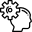
\includegraphics[width=2\baselineskip]{./viz/icons/Think.png}
      }
      {\ifthenelse{\equal{#1}{Homework}}
        {
          
\includegraphics[width=2\baselineskip]{./viz/icons/Homework.png}  
        }
       {
          \ifthenelse{\equal{#1}{Warning}}
            {
              
\includegraphics[width=2\baselineskip]{./viz/icons/Warning.png} 
            }
            {
            
            }
       }
      }%
\end{minipage}%
\begin{minipage}[ht]{0.75\linewidth}
}
{
\end{minipage}
}

\newenvironment{HIGHLIGHT}
{
\begin{mdframed}[backgroundcolor=cyan!10]
}
{
\end{mdframed}
}

\cleardoublepage
%===============================
\chapter*{Course Overview}
%==============================
\textbf{Data Analysis with R} is a 15 hour intensive program wherein the participants will ``learn by doing``. In this regard, two case studies will be shared, which will be prepared from 
  \begin{itemize}
    \item  \texttt{\url{https://www.kaggle.com/datasets}}
  \end{itemize}
\noindent The idea is that participants apply the techniques that they learn during the first six sessions, on the cases and prepare a presentation of their findings for the last two sessions. Also the participants will be expected to submit their R code before the last two sessions. Each case will require the participants to spend approximately 20-25 hours.

%==============================
\section*{Course Plan}
%==============================  
\begin{enumerate} 
    \item \textbf{Introduction to R (3 hours)}
     In the introduction sessions we will cover the following
    \begin{itemize}
      \item Setup R and Introduction to RStudio 
      \item Reading files in R. Introduction to data frames and basic operation on Data frames 
    \end{itemize}
    
    \item \textbf{Data Processing in R (1.5 hours)}
    
In these sessions we will cover different control structures in R. The participants will learn to write their first ``R function'' and ways to clean, aggregate and transform data:
    \item \textbf{Exploratory Data Analysis and Data Visualization in R (3 hours)}
    
In these sessions the participants will learn how to compute summary statistics of data in R, visualize datasets and learn to understand and explain ``the story of the dataset''
    \item \textbf{Statistical Modelling in R (1.5 hours)}
    
In these sessions, the participants will learn how to build a linear regression model on a multivariate dataset and interpret its results.
    \item \textbf{Case Analysis (6 hours)}
    
In these sessions, the participants will present, analyse and brainstorm on the application of different methods that they have been introduced to in the previous sessions, namely data processing, data exploration, data visualization and predictive modelling to two real world datasets.
  \end{enumerate}

%===============================  
\subsection*{The Book}
%===============================  
    % add the image of the reference book
    \begin{figure}[ht]
      \centering
      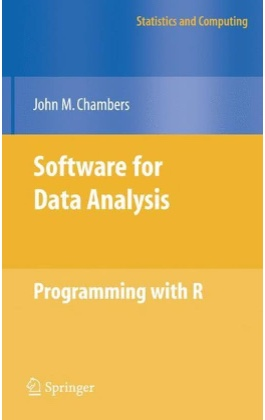
\includegraphics[width = 8 cm]{./viz/ext/book_intro_toR.jpeg}
    \end{figure}

    %add table for mapping between sessions and book 
    \begin{center}
      \begin{tabular}{ |c|c|c| } 
        \hline
          \textbf{\large Session} & \textbf{\large Chapters in the Book}  \\
        \hline   
          1 &  1, 2, 6.1, 6.2 \\
        \hline
          2 & 3, 6.3, 6.4, 6.5, 6.6, 6.7\\
        \hline  
          3 &  7 \\
        \hline
          4 & 6.8, 6.9, 6.10 \\
        \hline       
      \end{tabular}
    \end{center}
%==============================
% End of section book
%==============================

%================================
% End of chapter course overview
%=================================


%===============================
\tableofcontents
%===============================
\cleardoublepage
\thispagestyle{empty}
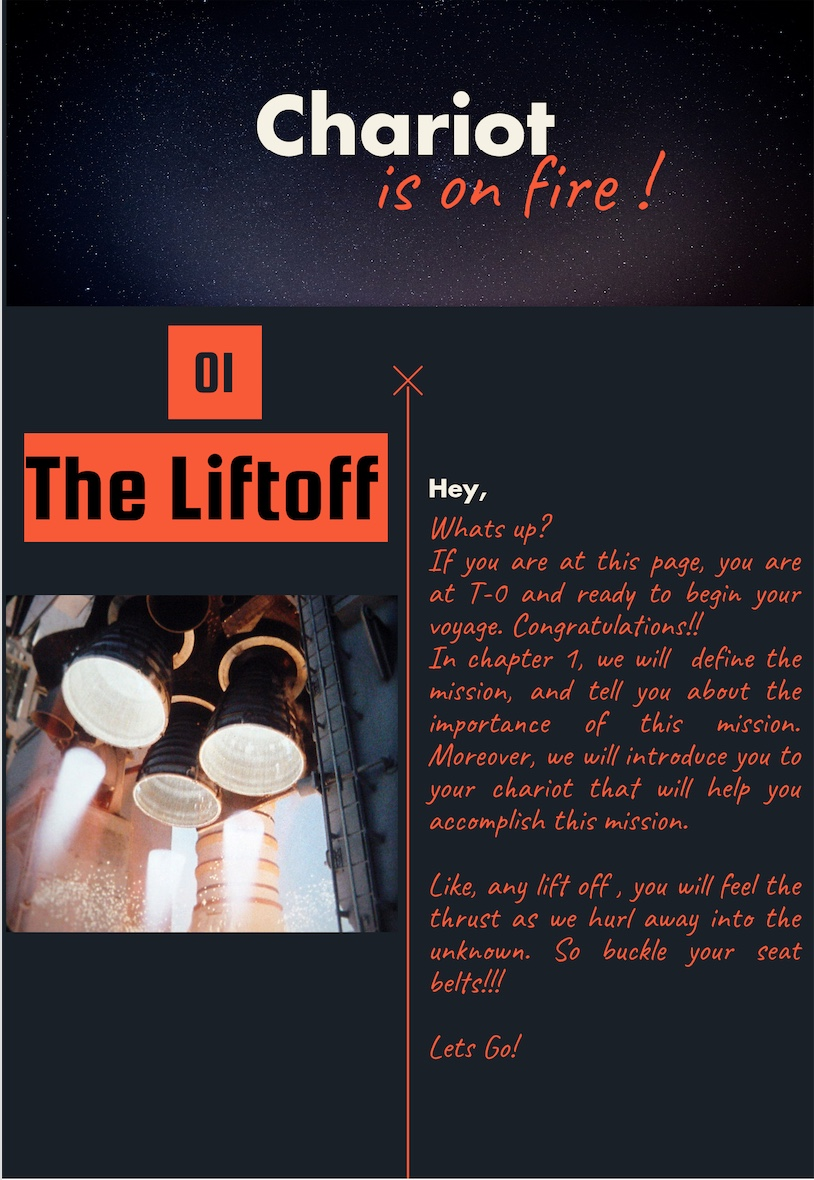
\includegraphics[width = 17 cm]{./viz/ext/Liftoff.jpeg}

\newpage
%=======================================
\chapter{The Liftoff}
%=======================================

% !Rnw root = main.Rnw


% !Rnw root = Introduction.Rnw
%==============================
\section{The Mission}
%==============================
\begin{HIGHLIGHT}
\par\noindent{
{\centering\textbf{\emph{\Huge ``Data Exploration''}} \\}
\vspace{\baselineskip}
\textbf{Data Exploration} entails the following activities:
\begin{enumerate}
      \item Formulation of  meaningful questions
      \item Organization of data in a way to answer the questions
\end{enumerate}
}
\end{HIGHLIGHT}
\begin{HIGHLIGHT}
\par\noindent{
\noindent Any real world entity can be treated as an object. 

\noindent Every object has a set of attributes.

\noindent The attributes of an object can be assigned values.
}
\end{HIGHLIGHT}

\noindent For example, a student is an object. A student can have \emph{age, gender, score} etc.. as attributes. Some of these values can be numeric, for example age and score, while other attributes can be categorical, for example gender.  When we collect attribute values for multiple (possibly similar) objects, we end up getting a data set. 
\begin{HIGHLIGHT}
\par\noindent{
\noindent The tabular representation of such data is one where the rows correspond to different objects, the columns correspond to the attributes of these objects and each cell corresponds to the attribute value for the object. 
}
\end{HIGHLIGHT}

\noindent Data exploration is the step, in which we try to identify patterns in the data thereby leading us to prove or disprove our hypothesis about the objects. For example, if we constructed a hypothesis that \emph{female students score higher than male students}. Then, in order to prove or disprove it we would have to first collect the data, organize it, and then try to find patterns in the data that would confirm the correctness/incorrectness of the hypothesis.  

\newpage
%=========================================
\subsection{Stages of Data Exploration}
%=========================================
\begin{HIGHLIGHT}
\par\noindent{
\emph{``It is as well to remember the following truths about models: all models are wrong; some models are better than others [George Box said more useful]; the correct model can never be known with certainty; and the simpler a model the better it is!''}
}
\end{HIGHLIGHT}

\begin{figure}[ht]
 \centering
    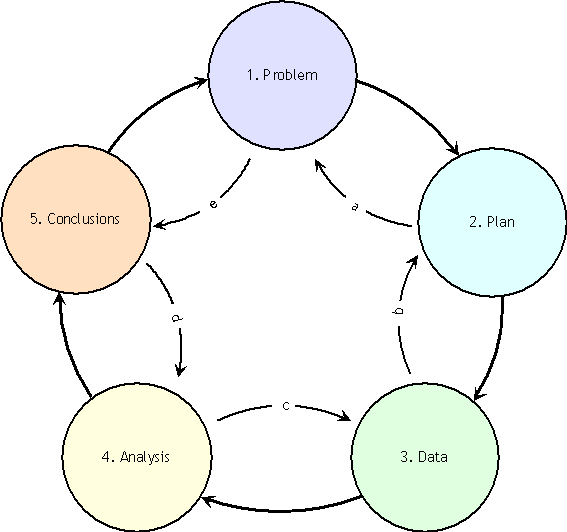
\includegraphics[width = 13 cm]{./viz/ext/ppdac.png}
\end{figure}

\begin{HIGHLIGHT}
\par\noindent{
\emph{``The purpose of the Conclusion stage is to report the results of the study in the language of the Problem. Concise numerical summaries and presentation graphics [tabulations, visualizations] should be used to clarify the discussion. Statistical jargon should be avoided. As well, the Conclusion provides an opportunity to discuss the strengths and weaknesses of the Plan, Data and Analysis especially in regards to possible errors that may have arisen'' Mackay and Oldford (2000)}
}
\end{HIGHLIGHT}
\newpage
%=========================================
\subsection{The Geometry of Data}
\label{sec:GeomOfData}
%=========================================
\begin{HIGHLIGHT}
\par\noindent{
\noindent In order to find patterns among objects of interest, we should be able to identify similar objects. One advantage of finding similar objects is that it allows us to find smaller cohorts of objects within which we can try to find patterns, that may have been non-existent in the larger group. 
}
\end{HIGHLIGHT}

\noindent For example, we may observe from the student data that gender does not correlate to score, but if we group the data by age, we may see that for certain age groups, gender does correlate with score. 

\begin{HIGHLIGHT}
\par\noindent{
\noindent It is important to compare objects by considering all their attributes. In order to analyze or compute on all attribute of an object, we need to give it an abstract representation. This is achieved by \textbf{\emph{representing data in the Cartesian coordinate system}} where each coordinate corresponds to an attribute. 
}
\end{HIGHLIGHT}

\noindent This is fairly easy when the attributes take a numeric value, for example if age = 17 and score = 75, its Cartesian coordinate representation would be (17,25).  

\noindent The representation gets a bit complicated for categorical attributes. In order to give it a Cartesian coordinate representation, we need to map each attribute value to a number. However a number system also has the inherent concept of ordering wherein assigning a higher number to something means assigning higher weight to it.
So, for the gender attribute, if we were to map the attribute value ``Male'' to 1 
and ``Female'' to 2, internally this means that we are assigning a higher value to the attribute value ``Female''

\noindent The correct way to do this is to treat each of the attribute values as representing a coordinate axis, such that when an attribute value is associated with an object it gets a value 1 and all other attribute values are set to 0. This is best explained by an example.

 \begin{center}
      \begin{tabular}{ |c|c|c|c|c| } 
        \hline
          \textbf{Id} & \textbf{Age} & \textbf{Gender} &  \textbf{Score} \\
        \hline   
          001 & 11 & M & 75\\
        \hline
          002 & 8 & F & 40\\
        \hline  
          003 & 10 & F & 82\\
        \hline
          004 & 15 & M  & 90\\
        \hline       
      \end{tabular}
    \end{center}

Now, the Cartesian coordinate representation of this data is shown in the table. $X1,X2,X3,X4$ are the coordinate axis.

 \begin{center}
      \begin{tabular}{ |c|c|c|c|c|c| } 
        \hline
          \textbf{Id} & \textbf{Age (X1)} & \textbf{isMale (X2)} &  \textbf{isFemale (X3)} & \textbf{Score (X4)} \\
        \hline   
          001 & 11 & 1 & 0 & 75\\
        \hline
          002 & 8 & 0 & 1 & 40\\
        \hline  
          003 & 10 & 0 & 1 & 82\\
        \hline
          004 & 15 & 1 & 0 & 90\\
        \hline       
      \end{tabular}
    \end{center}

\begin{figure}[ht]
 \centering
    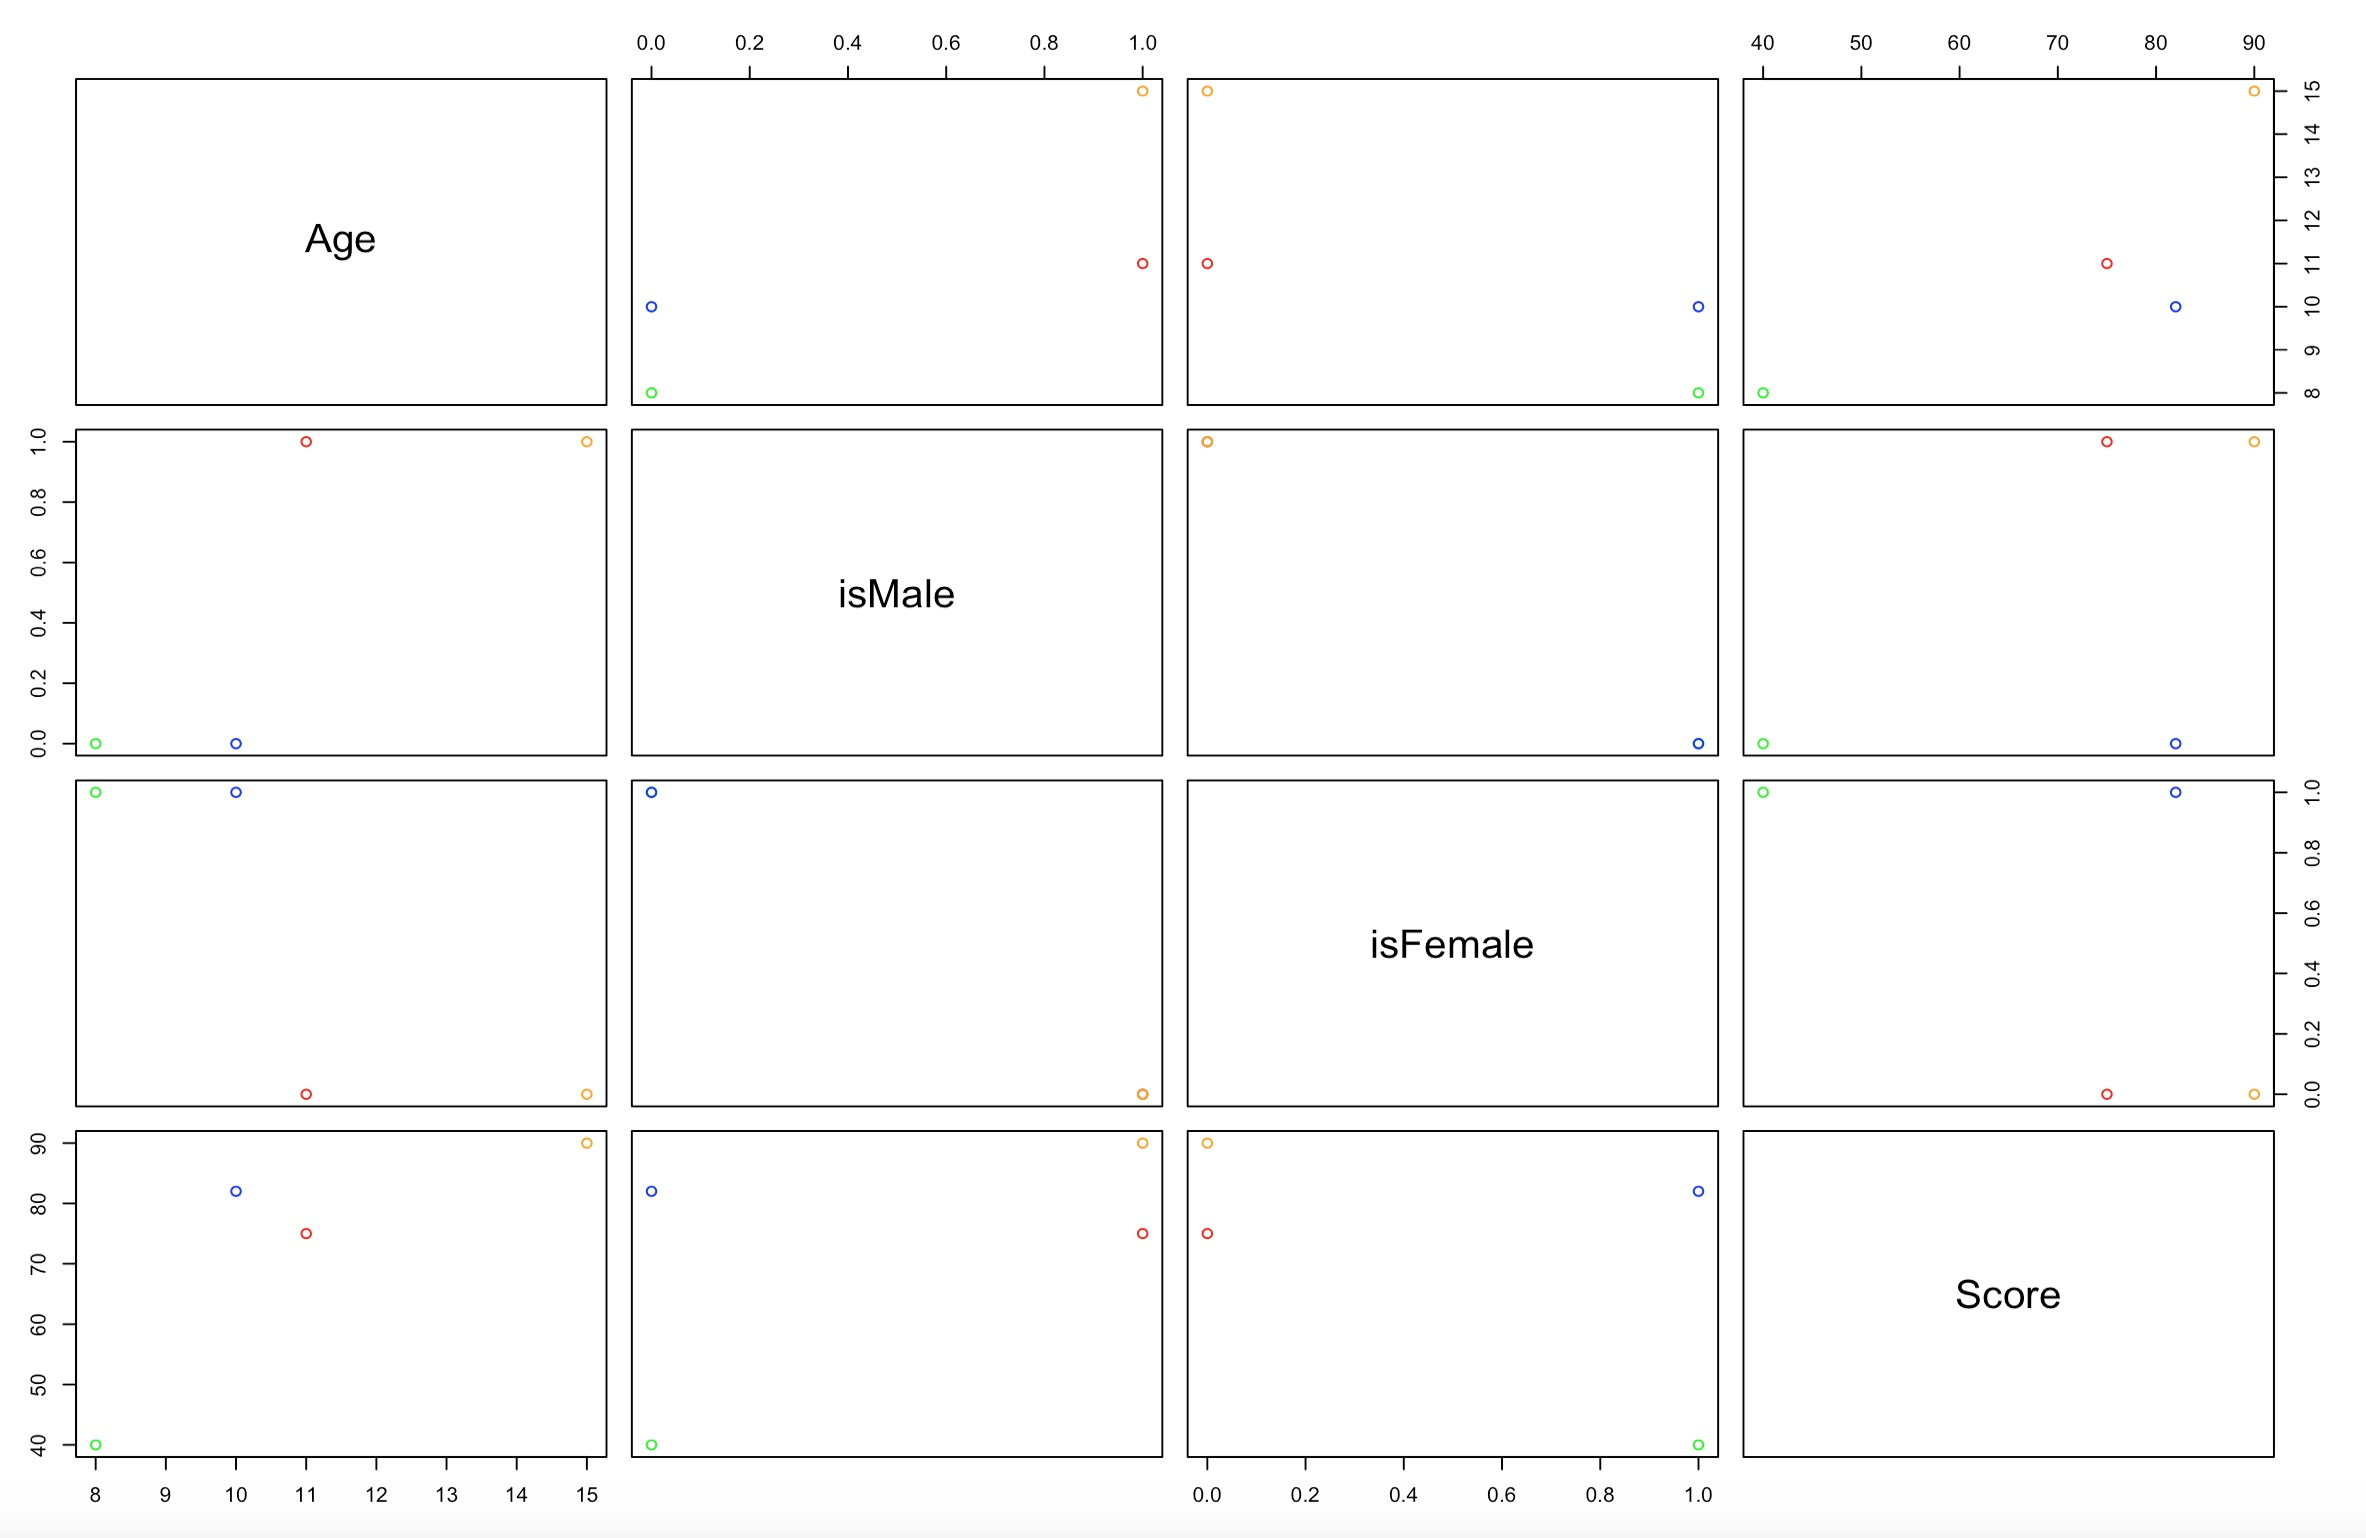
\includegraphics[width = 15 cm]{./viz/ext/ScatterplotMatrix.jpeg}
\end{figure}

\noindent Visualization of data in the Cartesian coordinate system , when the number of dimensions is more than three, is quite challenging. A easy workaround is a 2-D pairwise visualization of attributes. 

\begin{DIY}{Think}
Explain the plot.
\end{DIY}
%=========================================
\subsection{Challenges of Data Exploration}
%=========================================
\begin{HIGHLIGHT}
\par\noindent{
{\centering\textbf{\emph{``Lies, Damned Lies and Statistics''}} \\}
\vspace{\baselineskip}
\noindent The analysis stage of data exploration can be significantly hampered by
\begin{itemize}
  \item inadequate or unrepresentative data
  \item misleading visualization of results
\end{itemize}
This can lead to inadequate reasoning on the basis of results and therefore drawing of incorrect conclusions.
}
\end{HIGHLIGHT}

\begin{DIY}{Think}
Argue why the example in section \ref{sec:GeomOfData} poses challenges to data exploration.
\end{DIY}

\begin{DIY}{Homework}
Explore the data set in exercise1.csv.
Which \emph{Stages of Data Exploration} did you apply while exploring the data set in exercise1.csv?
What challenges did you face in your exploration?
\end{DIY}
\newpage
%=============================
\subsection{Data and Society}
%=============================
\begin{figure}[ht]
 \centering
    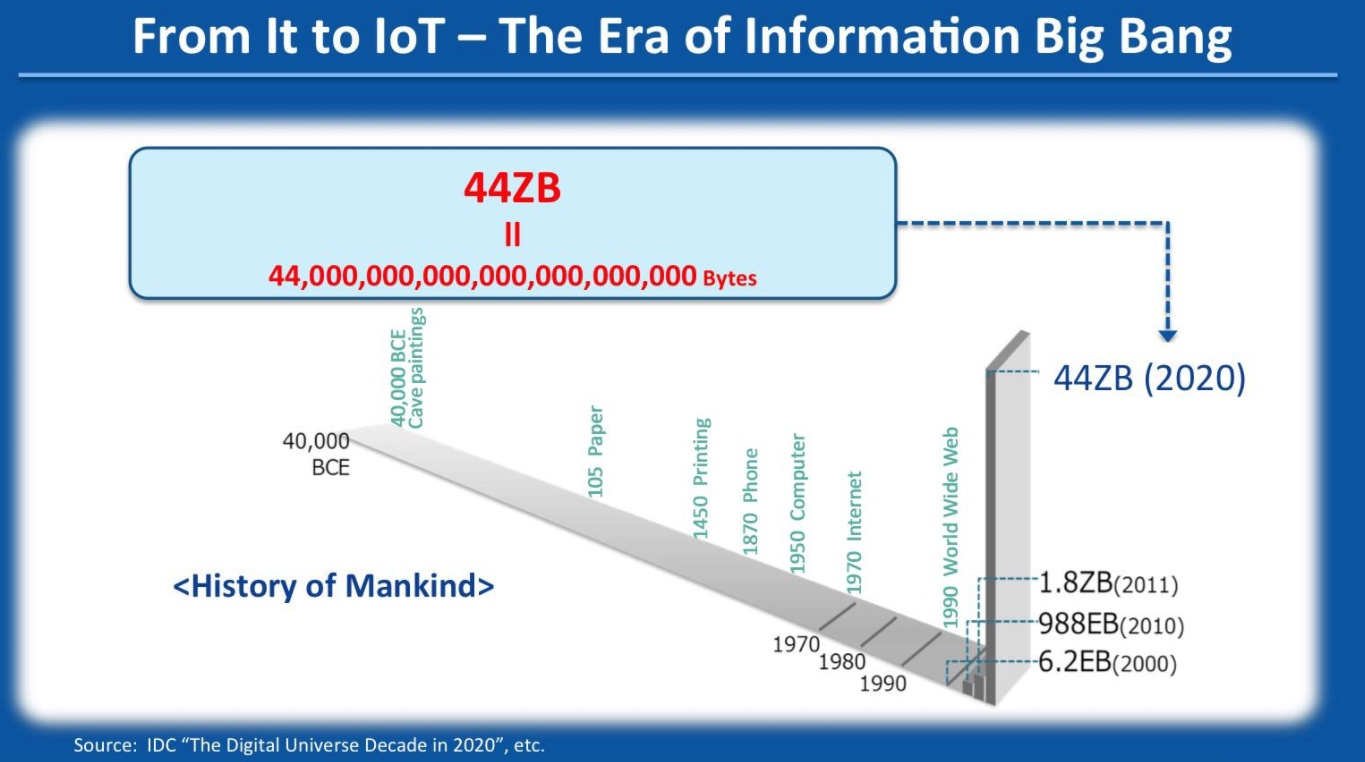
\includegraphics[width = 15 cm]{./viz/ext/DataVolumesVSHumanHistory.jpeg}
\end{figure}

\begin{DIY}{Think}
It is true that data is ubiquitous to modern society and is being generated at an unprecedented scale at high \textbf{\emph{volumes}}, \textbf{\emph{velocity}} and \textbf{\emph{variety}} (the \textbf{3V's}). Try categorizing each of the data source in the info graphic ``\emph{Data Never Sleeps 5.0}''
\begin{itemize}
  \item into one of the \textbf{3V's}  
  \item \textbf{\emph{high noise-to-signal}} ratio source v/s \textbf{\emph{low noise-to-signal}} ratio source
  \item sources where high volume \textbf{\emph{correlates}} to better insights 
\end{itemize}
\end{DIY}

\begin{DIY}{Homework}
Read Section 19 of the \emph{Statistical Analysis Handbook}
\end{DIY}

\begin{DIY}{Think}
Argue why the \textbf{4'th V} that you have just read about necessitates \emph{data exploration}
\end{DIY}

\begin{figure}
 \centering
    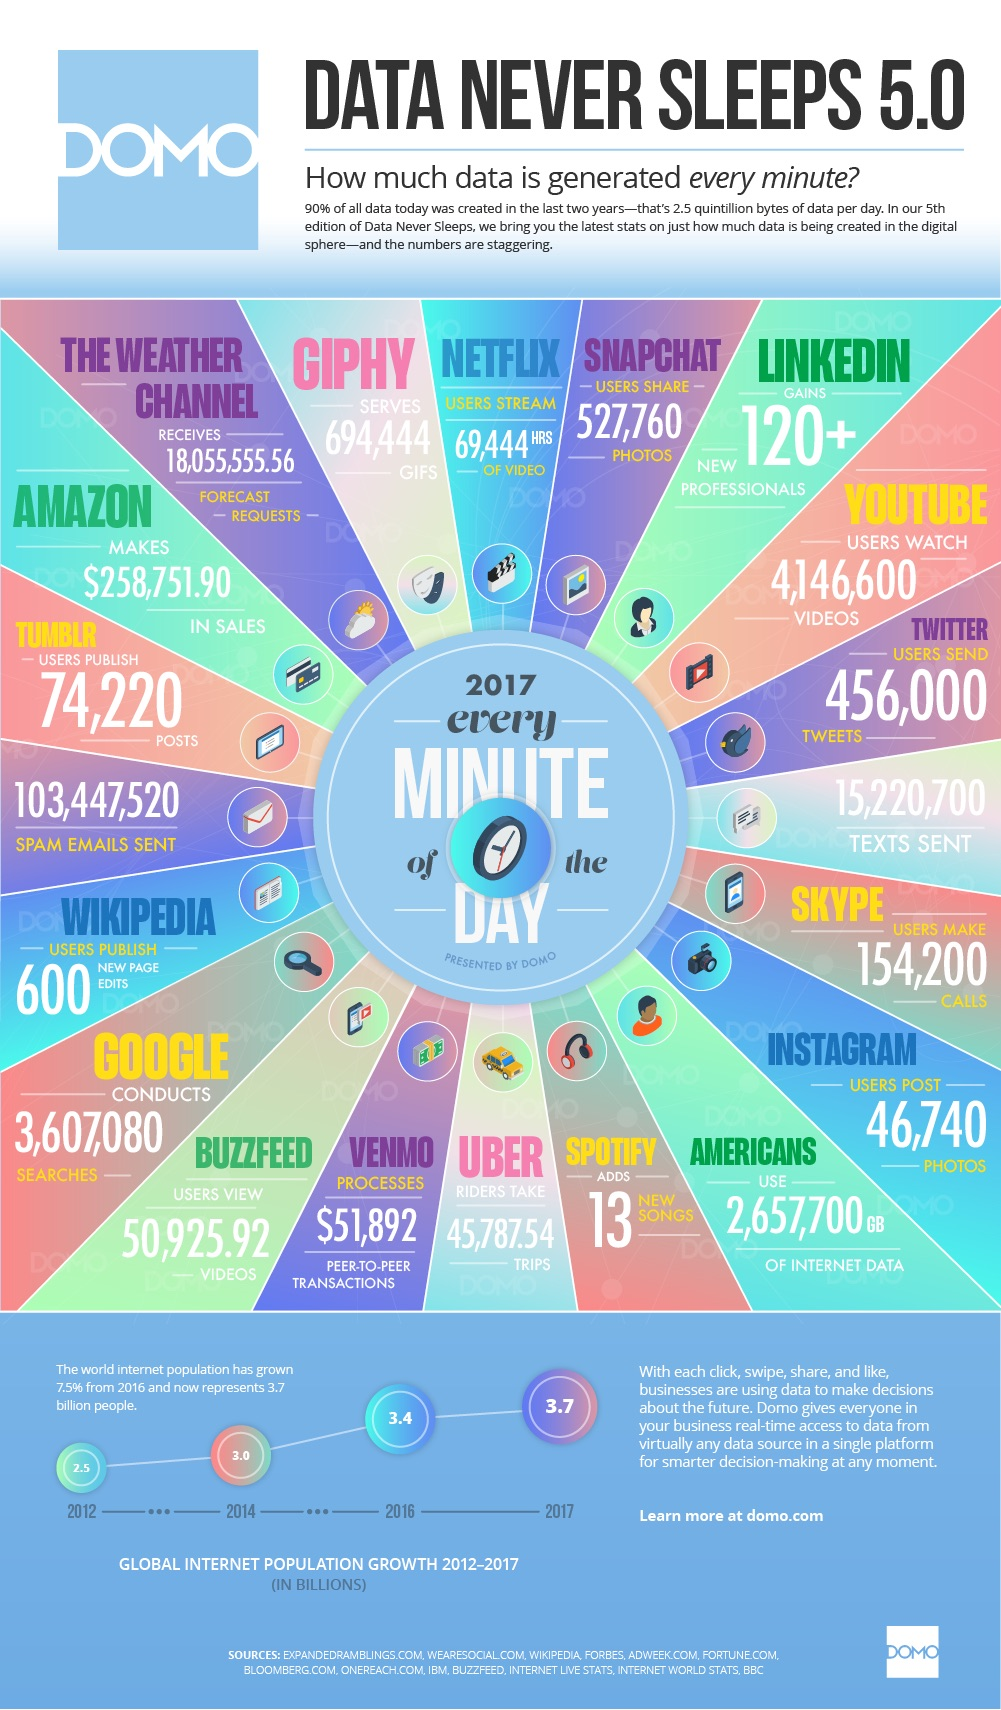
\includegraphics[width = 13 cm]{./viz/ext/dataeachday2017.jpg}
\end{figure}

\newpage
%=========================================
\subsection{Software for Data Exploration}
%=========================================
\begin{HIGHLIGHT}
\par\noindent{
{\centering\textbf{\emph{\Large ``Trustworthy, Flexible and Efficient Software: The Prime Directives''}} \\}
\vspace{\baselineskip}
\noindent The task of data exploration requires a tool that allows a user to ask meaningful questions about their applications quickly and flexibly. A wide range of techniques is needed to facilitate stages 1-4 of data exploration thereby requiring the data exploration tool to be flexible. Moreover, the tool should be able to provide answers to the questions asked ``\emph{within an acceptable time frame}''. The \textbf{3V's}, and the questions that are posed on the data, require complex transformations and computations on the data, whose correctness cannot be often verified by direct observation of the results in stage 5. Therefore, it is imperative that the underlying implementations of the transformations and computations (which is often \textbf{\emph{encapsulated}}) are correct.
}
\end{HIGHLIGHT}

\begin{DIY}{Think}
How does Microsoft Excel provide \textbf{\emph{Abstraction via Encapsulation}}. Think of an example where the trustworthiness comes into play.
\end{DIY}

\begin{DIY}{Warning}
It is extremely hard to achieve \emph{trustworthiness}, \emph{flexibility} and \emph{efficiency} at the same time. As you go ahead in the course try to identify trade-offs between the three directives in R.  
\end{DIY}




% !Rnw root = Introduction.Rnw
%==========================
\section{Why R?}
%==========================
\noindent Before delving into the question of \emph{why R?}, let us first take a look at how R fares with respect to to its competitors.The following two plots show the results of two surveys conducted in the year 2017. The first plot shows the result of a similar survey, conducted worldwide, by Kaggle.The second survey was conducted by O'Rielly in Europe and shows the popularity of different tools among data analysts/scientists.As is evident from both plots, R is a highly popular tool among data analysts/scientists.

    % Figure to demonstrate popularity of R in Kaggle surveys
    \begin{figure}[ht] % Figure to demonstrate popularity of R in O'Rielly surveys
      \centering
      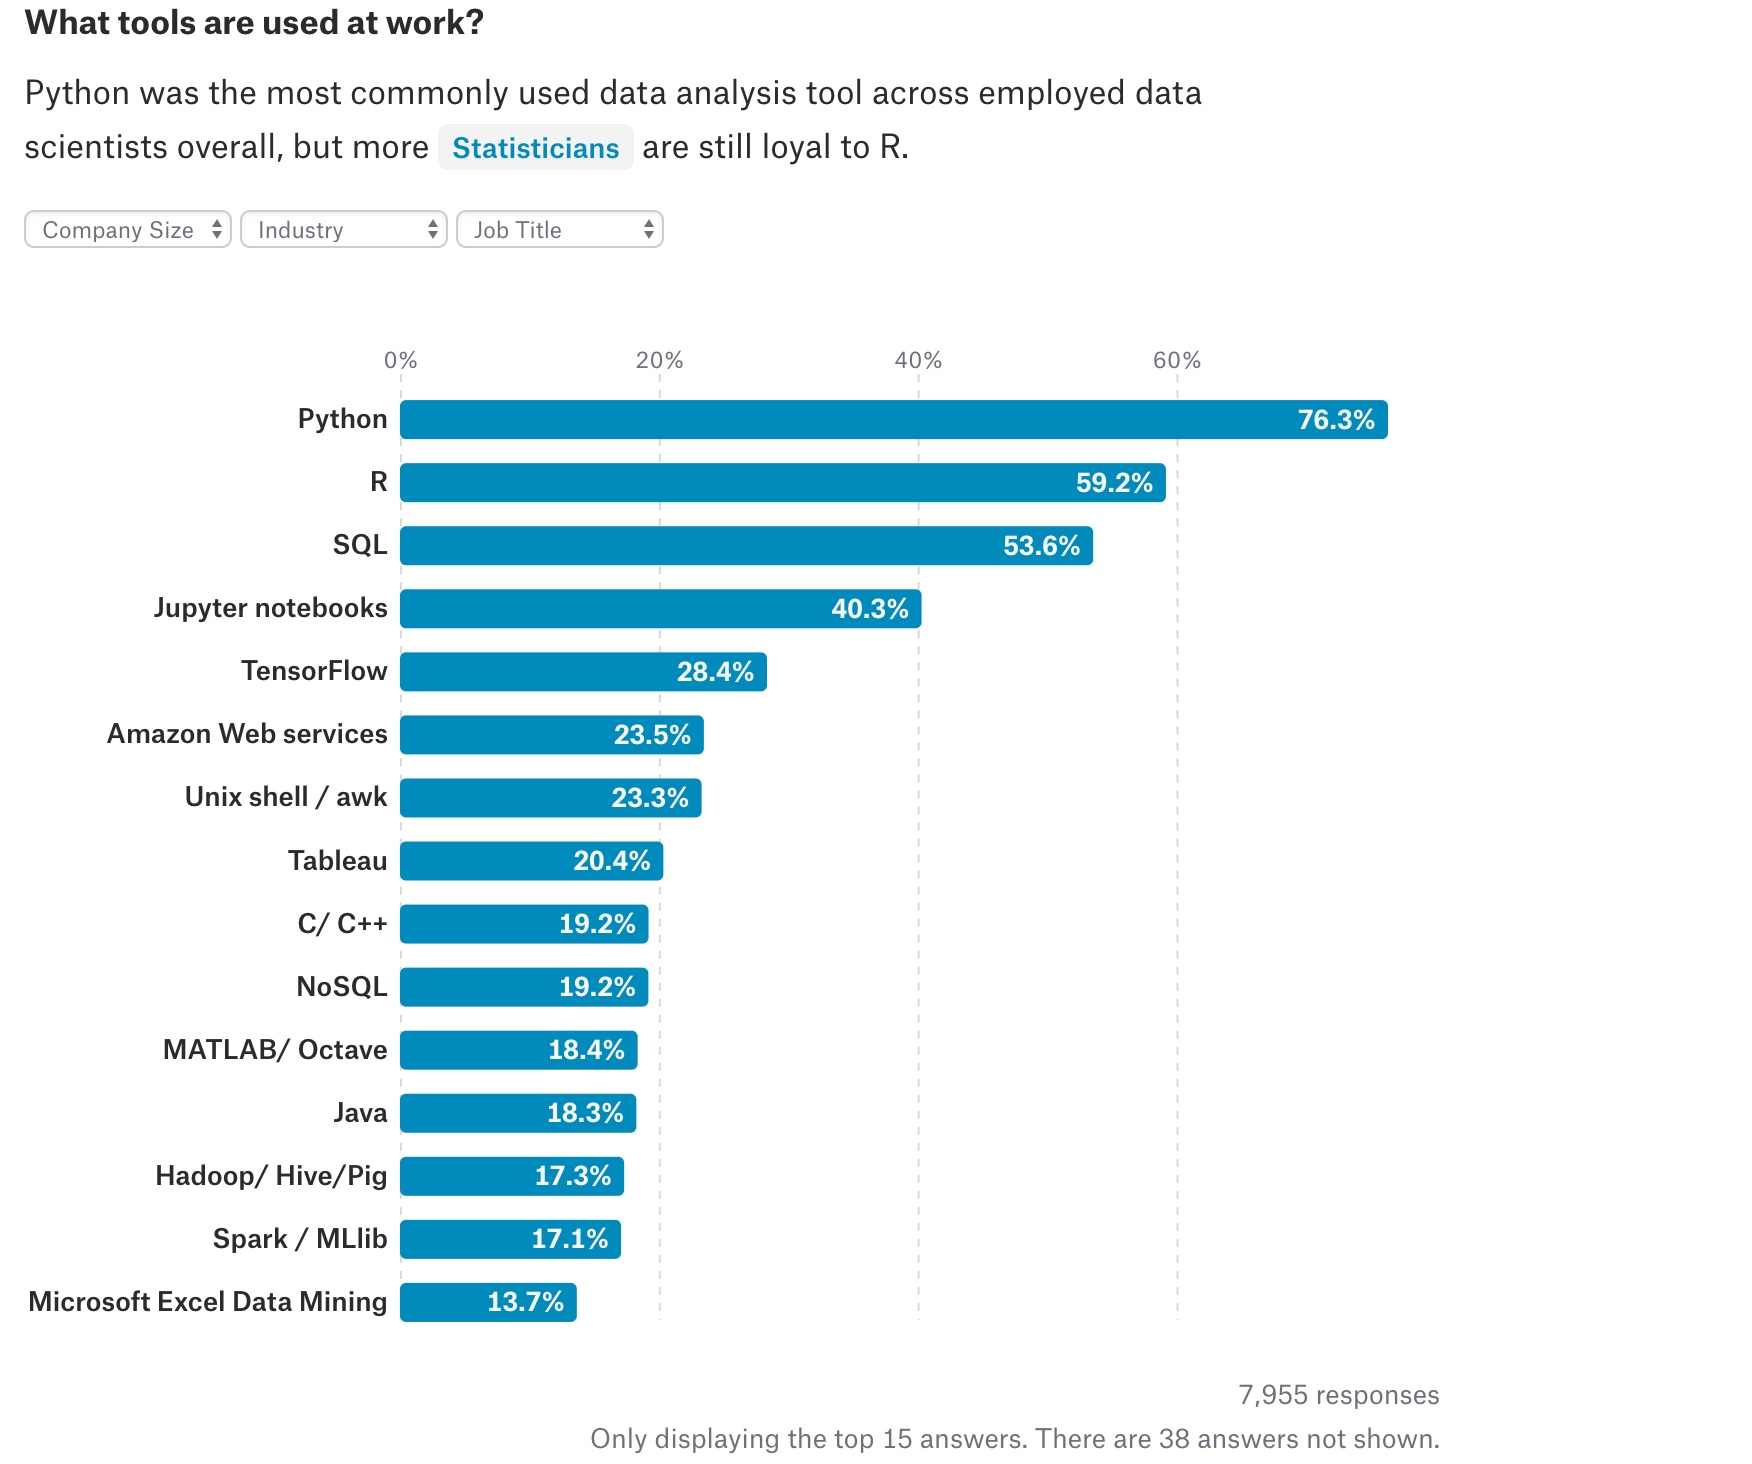
\includegraphics[width = 15 cm]{./viz/ext/Kaggle_DS_Tools_Survey.jpeg}
    \end{figure}

    \begin{figure}[ht] % Figure to demonstrate popularity of R in O'Rielly surveys
      \centering
      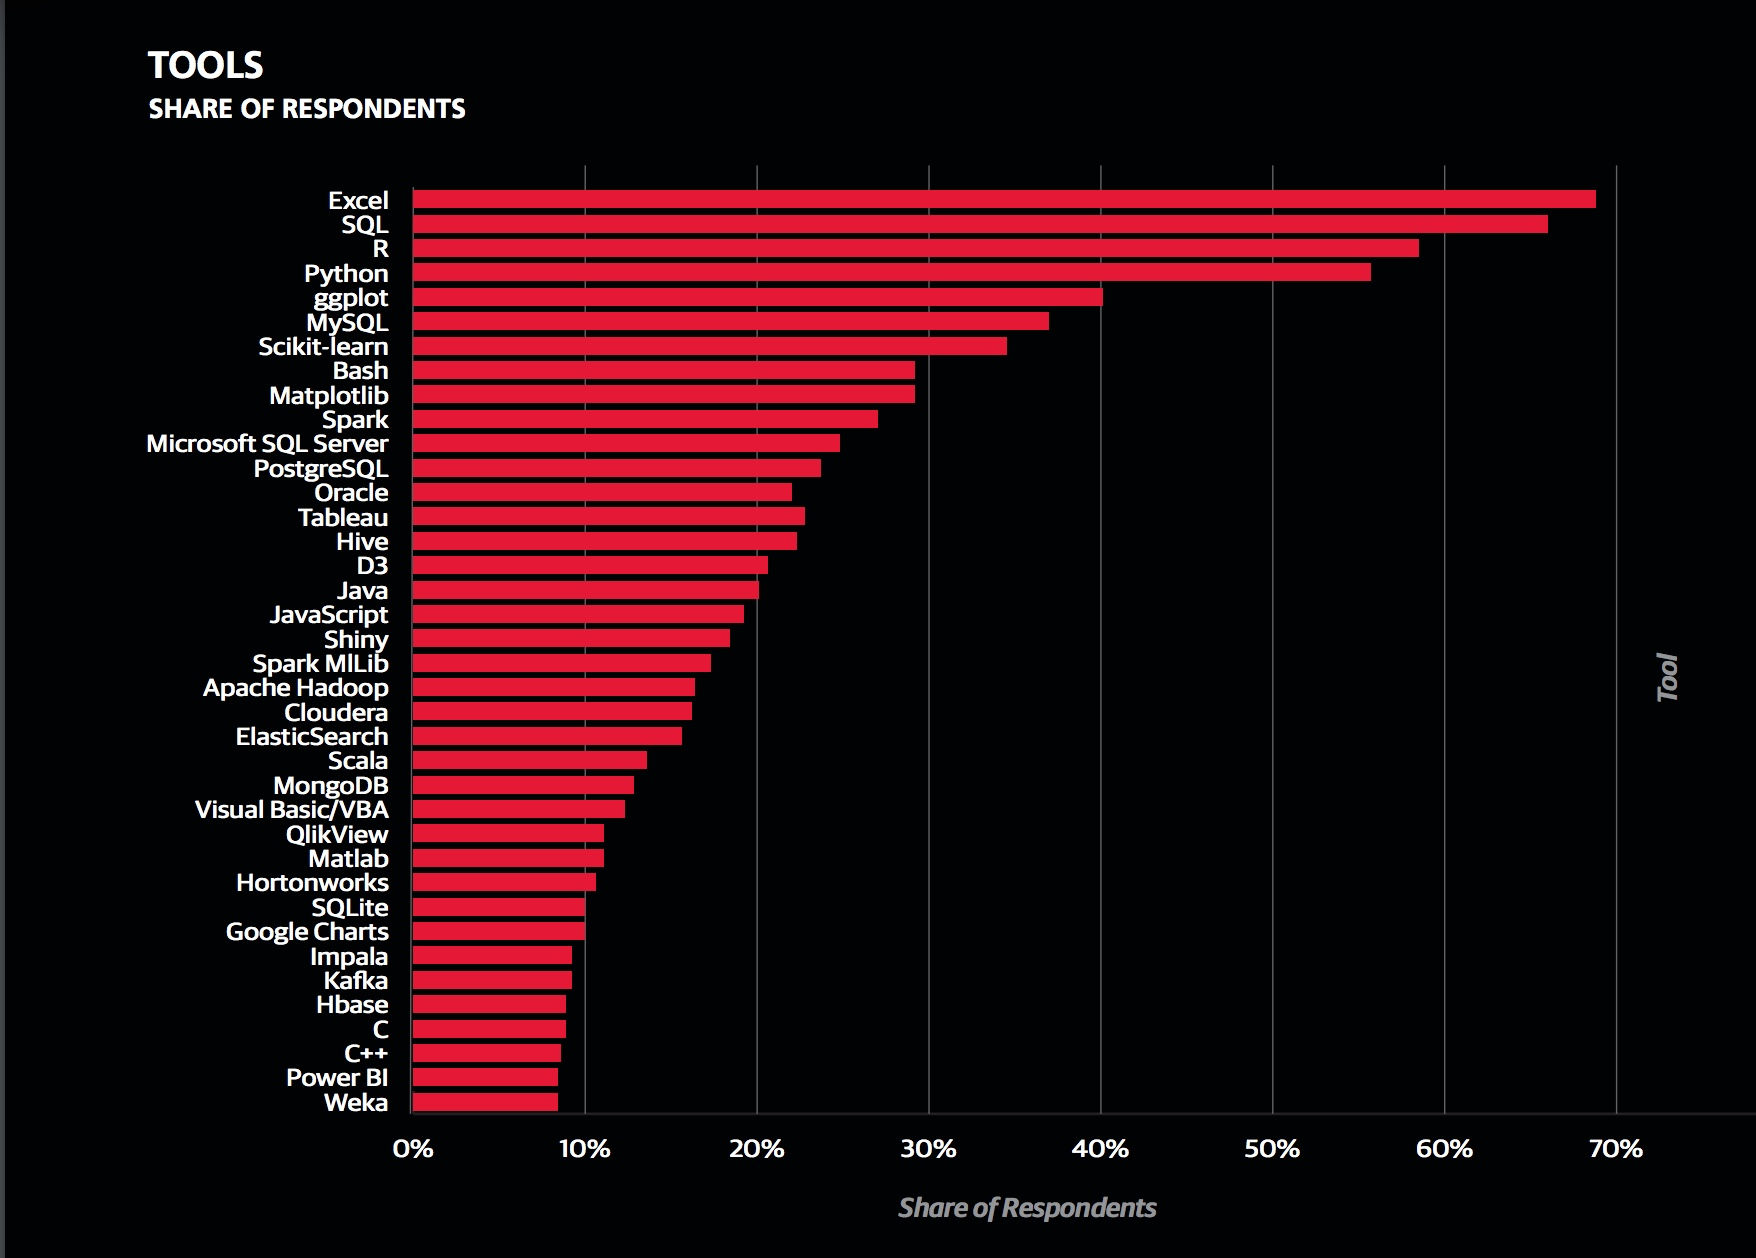
\includegraphics[width = 15 cm]{./viz/ext/OR_DS_Tools_Survey.jpeg}
    \end{figure}
    
\begin{DIY}{Think}
\emph{Think like an Analyst:} Criticize the plots in terms of their inadequacy to provide the complete information. Argue, why and how would this lead to drawing of incorrect conclusions. 
\end{DIY}

\begin{DIY}{Homework}
Read the reports
\begin{enumerate}
  \item \textbf{``European Data Science Salary Survey''} published by O'REILLY in 2017
  \item \textbf{``The State of Data Science \& Machine Learning''} published by Kaggle in 2017
\end{enumerate}
and get yourself acquainted with \emph{stage 5} of the data exploration process.
\end{DIY}

%================================  
\subsection{A Brief History of R}
%================================
\begin{itemize}
  \item \textbf{1976}: Statistical programming language S developed at Bell Labs since 1976 (at the same time as UNIX)
  \item \textbf{1993}: Research project in Auckland, NZ  by R. Gentleman and R. Ihaka
  \item \textbf{1995}: Released as an open-source software - generally compatible with the ``S'' language
  \item \textbf{1997}: R core group formed
  \item \textbf{2000}: R 1.0 released
  \item \textbf{2004}: First international user conference in Vienna
  \item \textbf{2013}: R 3.0.0 released
  \item \textbf{2017}: R at version 3.4.3
\end{itemize}

\newpage
%================================
\subsection{Concepts for Programming with R}
%================================
%================================
\subsubsection{Functional Programming}
%================================
\begin{HIGHLIGHT}
\par\noindent{
Software in R is written in a \emph{functional style} that 
emphasizes on \emph{encapsulating computations via functions} thereby allowing the programmer to create \emph{abstractions by separating behavior from implementation}.}
\end{HIGHLIGHT}

\begin{DIY}{Think}
If you are given a set of $N$ numbers whose average needs to be computed, think about how would the functional programming approach allow you to achieve abstraction and what would be its benefit?
\emph{Hint:} Think about how would the computation of average differ when $N$ numbers are given in one go (\textbf{\emph{batched input}}) as opposed to when you get every number one after the other (\textbf{\emph{streaming input}})
\end{DIY}

%================================
\subsubsection{Classes and Methods}
%================================
\begin{HIGHLIGHT}
\par\noindent{
\emph{``Functions in R return objects'}'. Therefore any kind of \textbf{\emph{data in R is always an object}}. While functions facilitate abstraction by encapsulating implementation of computation, \emph{classes encapsulate objects}. \emph{Methods in R knit together functions and classes}.   
}
\end{HIGHLIGHT}
%================================
\subsubsection{Data Frames}
%================================
\begin{HIGHLIGHT}
\par\noindent{
A \emph{data frame} is organization of data as observations (rows) and attributes (columns). Data frames are one of the predominant data structures in R. Moreover, they are synonymous with the tabular representation of data as is found in spreadsheets and relational database systems. Such similarity in representation of data enables seamless integration between R and most spreadsheets and RDBMS systems. 
}
\end{HIGHLIGHT}
%================================
\subsubsection{Ecosystem}
%================================
\begin{HIGHLIGHT}
\par\noindent{
R is an open-source software, thereby providing access to source code sufficient to generate a working version of the software. R is distributed under a version of GPL (Gnu Public License). An effect of this is that R has a thriving community of contributors and active users. Users, seek out existing implementation of data analysis/modeling techniques from a repository called \textbf{\emph{CRAN}} (\textcolor{cyan}{\url{https://cran.r-project.org/}}). When they do not find an existing implementation that suits their needs, they create their own implementations, \emph{package} these implementations and contribute them back to CRAN. As a result of this CRAN today boasts a total of 12000+ packages. Please see the plot below that shows the growth in number of CRAN packages over time. This has resulted in R being unparalleled in the number of options it provides for data analysis. Moreover, R is the primary tool used for statistical research (and has been so for 20 years). Therefore, when new methods are developed, they are not just published as a paper - they are also published as an R package. This means R is always on the cutting edge of new technologies. Furthermore, R was designed as an interface language - a means to present a consistent language interface for algorithms written in other languages. Many packages work by providing R language bindings to other open-source software, making R a convenient hub for all kinds of algorithms and methods.     
}
\end{HIGHLIGHT}

\begin{figure}[ht] % Figure to demonstrate growth in number of CRAN packages over time
      \centering
      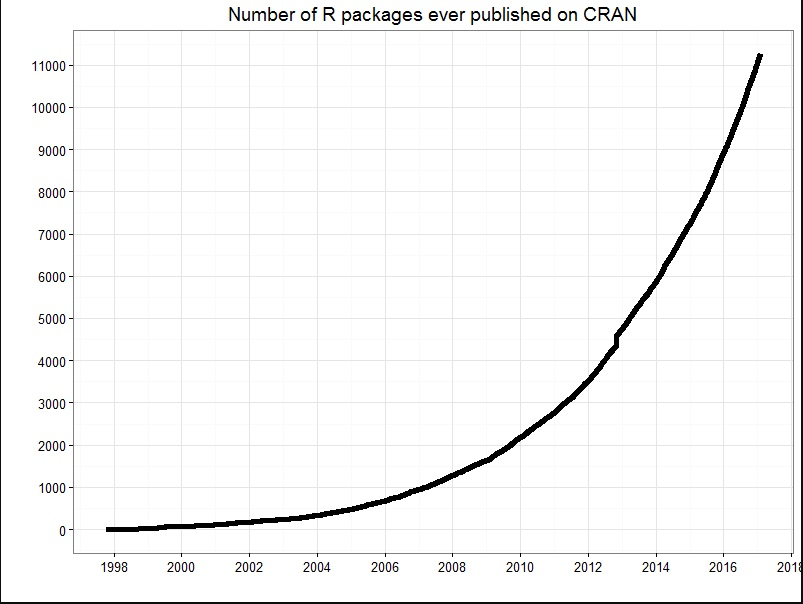
\includegraphics[width = 10 cm]{./viz/ext/numberofCRANpackages_over_Time.jpeg}
    \end{figure}

\begin{DIY}{Think}
Did you notice the sudden discontinuity in the curve around the year 2013? Can you think of what might have caused this?
\end{DIY}

\begin{DIY}{Think}
Argue \textbf{\emph{Why R}} satisfies \emph{the prime directives} and should therefore be our tool of choice for our mission of data exploration
\end{DIY}
    
\section{RStudio}

\begin{HIGHLIGHT}
\par\noindent{
\begin{DIY}{Homework}
Watch the video on \\
\textcolor{cyan}{\url{https://www.rstudio.com/resources/webinars/rstudio-essentials-webinar-series-part-1/}}\\
and install R and RStudio on the computer that you will be accessing during the sessions.
\end{DIY}
}
\end{HIGHLIGHT}

\begin{DIY}{Warning}
\textcolor{red}{It is important that the participants have R and RStudio installed on their computers before Session 1.}
\end{DIY}

\begin{DIY}{Homework}
Download the RStudio IDE Cheat Sheet and use it as a reference while working with RStudio. In order to download the Cheat Sheet, \emph{Open RStudio $>$ Go to  Help Menu $>$ Cheatsheets $>$ RStudio IDE Cheat Sheet}
\end{DIY}

\newpage
\includepdf[pages={1}]{./References/rstudio-ide.pdf}

\cleardoublepage
\thispagestyle{empty}

\includegraphics[width = 17 cm]{./viz/ext/Ascent_A.jpg}

\newpage
%=======================================
\chapter{The Ascent - PART A}
%=======================================

% !Rnw root = main.Rnw


% !Rnw root = Introduction.Rnw
%===============================
\section{Using R}
%===============================
\begin{HIGHLIGHT}
\par\noindent{
R is an \emph{interactive} environment, wherein the users gets immediate feedback (\emph{results}) for their instructions (\emph{expressions}). This is in contrast to programming languages like C++ or Java wherein a set of instructions (the program) has to be created and compiled before the results can be generated.In R, the interaction between the user and the system constitutes an \emph{R Session}. During an R session, the user provides \emph{expressions} to R for doing computations, displaying results, and creating objects for further use. R, first evaluates the expressions for its syntactic correctness and then performs the task, as specified by the expression. We will examine some basic expressions in the following sub-sections.     
}
\end{HIGHLIGHT}

At the \emph{console}, the user finds the \textbf{$>$} prompt where the user responds by typing and expression. Hereon, in this section every expression/set of expressions is mentioned in the gray box and is to be issued at the $>$ prompt in the console. Moreover, following the motto of this course ``learn by doing``, the reader is strongly encouraged to try out each of these expressions and \emph{read the corresponding help manual for each expression}. As is evident from the examples shown in this section, expressions are predominantly \textbf{\emph{function calls with a set of arguments}}.

\begin{HIGHLIGHT}
\par\noindent{
R, like Python, MATLAB etc is a \emph{dynamically typed language} which means that you won't have to define the type of the variable (which stores your data). As a result, the user can only focus on the \emph{data stored by the variable} rather than having to worry about \emph{how the data is stored in the variable}. This is in stark contrast to \emph{statically typed languages} like C++ and Java.      
}
\end{HIGHLIGHT}

\begin{DIY}{Think}
How does a R \emph{data frame} exemplify the \emph{dynamic typing} feature of R?
\end{DIY}
    
\begin{DIY}{Warning}
The dynamic typing feature of R  provides great flexibility but at what cost?
\end{DIY}



% !Rnw root = Introduction.Rnw
\newpage
%===============================
\section{Basic Data Types}
%===============================
\begin{HIGHLIGHT}
\par\noindent{
Objects are the center of computations in R, along with the function calls that create and use those objects.
}
\end{HIGHLIGHT}

\begin{DIY}{Think}
What are objects in R? Why are functions and objects dual to each other? 
\end{DIY}

\subsubsection{The $class()$ function}
\noindent Every object in R has a \emph{type} associated with it, which signifies the kind of data it contains e.g numbers, strings etc. The $class()$ function accepts an object as an argument and returns its type.

\subsection{Data Type for Boolean}
\subsubsection{The ``logical'' type}
\begin{knitrout}
\definecolor{shadecolor}{rgb}{0.969, 0.969, 0.969}\color{fgcolor}\begin{kframe}
\begin{alltt}
\hlkwd{class}\hlstd{(}\hlnum{TRUE}\hlstd{)}
\end{alltt}
\begin{verbatim}
## [1] "logical"
\end{verbatim}
\begin{alltt}
\hlkwd{class}\hlstd{(}\hlnum{FALSE}\hlstd{)}
\end{alltt}
\begin{verbatim}
## [1] "logical"
\end{verbatim}
\end{kframe}
\end{knitrout}
\subsection{Data Type for Numbers}
\subsubsection{The ``numeric'' type}
\begin{knitrout}
\definecolor{shadecolor}{rgb}{0.969, 0.969, 0.969}\color{fgcolor}\begin{kframe}
\begin{alltt}
\hlkwd{class}\hlstd{(}\hlnum{1}\hlstd{)}
\end{alltt}
\begin{verbatim}
## [1] "numeric"
\end{verbatim}
\begin{alltt}
\hlkwd{class}\hlstd{(}\hlnum{3.141593}\hlstd{)}
\end{alltt}
\begin{verbatim}
## [1] "numeric"
\end{verbatim}
\end{kframe}
\end{knitrout}
\subsection{Data Type for Strings}
\subsubsection{The ``character'' type}
\begin{knitrout}
\definecolor{shadecolor}{rgb}{0.969, 0.969, 0.969}\color{fgcolor}\begin{kframe}
\begin{alltt}
\hlkwd{class}\hlstd{(}\hlstr{"Carpe Diem"}\hlstd{)}
\end{alltt}
\begin{verbatim}
## [1] "character"
\end{verbatim}
\end{kframe}
\end{knitrout}
\subsection{Concatenating Strings}
\subsubsection{The $paste()$ function}
\begin{knitrout}
\definecolor{shadecolor}{rgb}{0.969, 0.969, 0.969}\color{fgcolor}\begin{kframe}
\begin{alltt}
\hlkwd{paste}\hlstd{(}\hlstr{"Data Analysis"}\hlstd{,}\hlstr{"with R"}\hlstd{,}\hlkwc{sep}\hlstd{=}\hlstr{","}\hlstd{)}
\end{alltt}
\begin{verbatim}
## [1] "Data Analysis,with R"
\end{verbatim}
\end{kframe}
\end{knitrout}



% !Rnw root = Introduction.Rnw
%===============================
\section{Coercion}
%===============================
\begin{HIGHLIGHT}
\par\noindent{
{\centering\textbf{\emph{logical, integer, numeric, character}} \\}
\vspace{\baselineskip}
\noindent An ordering of data types from simple to complex. \emph{Coercion} is the conversion from one type to another. However, coercion from any type to another is neither possible nor valid. The general rule for coercion is: \emph{Coercion from a a simple type to a more complex type is valid}
}
\end{HIGHLIGHT}
\subsubsection{The ``is'' and ``as'' methods}
The \emph{is} method can be used to test whether an object is from a given class.

\noindent The \emph{as} method can be used to coerce an object from one class to another.
\subsection{Coercion between Boolean and Numbers}
\begin{knitrout}
\definecolor{shadecolor}{rgb}{0.969, 0.969, 0.969}\color{fgcolor}\begin{kframe}
\begin{alltt}
\hlkwd{is.logical}\hlstd{(}\hlnum{TRUE}\hlstd{)} \hlcom{##check if the  data is of type logical}
\end{alltt}
\begin{verbatim}
## [1] TRUE
\end{verbatim}
\begin{alltt}
\hlkwd{as.numeric}\hlstd{(}\hlnum{TRUE}\hlstd{)} \hlcom{##coerce from logical to numeric}
\end{alltt}
\begin{verbatim}
## [1] 1
\end{verbatim}
\begin{alltt}
\hlkwd{is.numeric}\hlstd{(}\hlnum{10}\hlstd{)} \hlcom{##check if the data is of type numeric}
\end{alltt}
\begin{verbatim}
## [1] TRUE
\end{verbatim}
\begin{alltt}
\hlkwd{as.logical}\hlstd{(}\hlnum{10}\hlstd{)} \hlcom{##coerce form numeric to logical. }
\end{alltt}
\begin{verbatim}
## [1] TRUE
\end{verbatim}
\begin{alltt}
\hlcom{##Any number that is not equal to 0 will be coerced to FALSE  }
\hlkwd{as.logical}\hlstd{(}\hlnum{0}\hlstd{)} \hlcom{##coerce from numeric to logical. }
\end{alltt}
\begin{verbatim}
## [1] FALSE
\end{verbatim}
\begin{alltt}
\hlcom{##Any number that is equal to 0 will be coerced to TRUE }
\hlkwd{as.logical}\hlstd{(}\hlnum{0.013}\hlstd{)} \hlcom{##coerce from numeric to logical}
\end{alltt}
\begin{verbatim}
## [1] TRUE
\end{verbatim}
\end{kframe}
\end{knitrout}
\begin{DIY}{Think}
Give \emph{real world} examples of when would you need to coerce between Boolean and numbers.
\end{DIY}
\subsection{Coercion between Boolean and Strings}
\begin{knitrout}
\definecolor{shadecolor}{rgb}{0.969, 0.969, 0.969}\color{fgcolor}\begin{kframe}
\begin{alltt}
\hlkwd{is.logical}\hlstd{(}\hlnum{TRUE}\hlstd{)} \hlcom{##check if the data is of type boolean}
\end{alltt}
\begin{verbatim}
## [1] TRUE
\end{verbatim}
\begin{alltt}
\hlkwd{as.character}\hlstd{(}\hlnum{TRUE}\hlstd{)} \hlcom{##coerce boolean to strings}
\end{alltt}
\begin{verbatim}
## [1] "TRUE"
\end{verbatim}
\begin{alltt}
\hlkwd{is.character}\hlstd{(}\hlstr{"TRUE"}\hlstd{)}  \hlcom{##check if the data is of type string}
\end{alltt}
\begin{verbatim}
## [1] TRUE
\end{verbatim}
\begin{alltt}
\hlkwd{as.logical}\hlstd{(}\hlstr{"TRUE"}\hlstd{)} \hlcom{##coerce from string to boolean}
\end{alltt}
\begin{verbatim}
## [1] TRUE
\end{verbatim}
\begin{alltt}
\hlkwd{as.logical}\hlstd{(}\hlstr{"Data"}\hlstd{)} \hlcom{##coerce any arbitrary string to logical}
\end{alltt}
\begin{verbatim}
## [1] NA
\end{verbatim}
\end{kframe}
\end{knitrout}
\begin{DIY}{Warning}
As shown in the last example, R does not prevent the coercion of an arbitrary string to logical. It just generates NA. 
\end{DIY}

\begin{DIY}{Think}
Give \emph{real world} examples of when would you need to coerce between Boolean and strings.
\end{DIY}
\subsection{Coercion between Numbers and Strings}
\begin{knitrout}
\definecolor{shadecolor}{rgb}{0.969, 0.969, 0.969}\color{fgcolor}\begin{kframe}
\begin{alltt}
\hlkwd{as.character}\hlstd{(}\hlnum{1}\hlstd{)} \hlcom{## coerce from number to string}
\end{alltt}
\begin{verbatim}
## [1] "1"
\end{verbatim}
\begin{alltt}
\hlkwd{as.character}\hlstd{(}\hlnum{1.0023}\hlstd{)} \hlcom{## coerce from number to string}
\end{alltt}
\begin{verbatim}
## [1] "1.0023"
\end{verbatim}
\begin{alltt}
\hlkwd{as.numeric}\hlstd{(}\hlstr{"1"}\hlstd{)} \hlcom{## coerce from string to number}
\end{alltt}
\begin{verbatim}
## [1] 1
\end{verbatim}
\begin{alltt}
\hlkwd{as.numeric}\hlstd{(}\hlstr{"Data"}\hlstd{)} \hlcom{## coerce from string to number}
\end{alltt}


{\ttfamily\noindent\color{warningcolor}{\#\# Warning: NAs introduced by coercion}}\begin{verbatim}
## [1] NA
\end{verbatim}
\end{kframe}
\end{knitrout}
\begin{DIY}{Warning}
Note the difference in output in the last two cases. When a number is passed as a string to $as.numeric()$, it its able to detect the same and correctly coerces it to a number. 
\end{DIY}

\begin{DIY}{Think}
Give \emph{real world} examples of when would you need to coerce between Boolean and strings.
\end{DIY}


% !Rnw root = Introduction.Rnw
%===============================
\section{Operators}
%===============================
\begin{HIGHLIGHT}
\par\noindent{
In R, an operator is a function which can take one argument (unary operator) or two arguments (binary operator).
Like any function in R, \emph{an operator too has a return type}. 
}
\end{HIGHLIGHT}

\subsection{Arithmetic Operators}
\begin{knitrout}
\definecolor{shadecolor}{rgb}{0.969, 0.969, 0.969}\color{fgcolor}\begin{kframe}
\begin{alltt}
\hlnum{3} \hlopt{+} \hlnum{2} \hlcom{## the '+' operator to add two numbers}
\end{alltt}
\begin{verbatim}
## [1] 5
\end{verbatim}
\begin{alltt}
\hlnum{3} \hlopt{-} \hlnum{2} \hlcom{## the '-' operator to substract two numbers}
\end{alltt}
\begin{verbatim}
## [1] 1
\end{verbatim}
\begin{alltt}
\hlnum{3} \hlopt{*} \hlnum{2} \hlcom{## the '*' operator to multiply two numbers}
\end{alltt}
\begin{verbatim}
## [1] 6
\end{verbatim}
\begin{alltt}
\hlnum{3} \hlopt{/} \hlnum{2} \hlcom{## the '/' operator to divide two numbers}
\end{alltt}
\begin{verbatim}
## [1] 1.5
\end{verbatim}
\begin{alltt}
\hlnum{3} \hlopt{^} \hlnum{2} \hlcom{## the '^' operator to calculate exponent }
\end{alltt}
\begin{verbatim}
## [1] 9
\end{verbatim}
\begin{alltt}
\hlnum{3} \hlopt \hlnum{2} \hlcom{## the '%%' operator to calculate modulus}
\end{alltt}
\begin{verbatim}
## [1] 1
\end{verbatim}
\end{kframe}
\end{knitrout}
\begin{DIY}{Think}
What is the return type for arithmetic operators
\end{DIY}

\begin{DIY}{Think}
Try using the arithmetic operators '+' and '*' on operands of type logical. Explain your observations
\end{DIY}

\begin{DIY}{Think}
Try using the arithmetic operators on operands of type character. 
\end{DIY}

\subsection{Comparison Operators}
\begin{knitrout}
\definecolor{shadecolor}{rgb}{0.969, 0.969, 0.969}\color{fgcolor}\begin{kframe}
\begin{alltt}
\hlnum{3} \hlopt{<} \hlnum{2} \hlcom{## less than comparison operator  }
\end{alltt}
\begin{verbatim}
## [1] FALSE
\end{verbatim}
\begin{alltt}
\hlnum{3} \hlopt{<=} \hlnum{3} \hlcom{## less than equal to comparison operator}
\end{alltt}
\begin{verbatim}
## [1] TRUE
\end{verbatim}
\begin{alltt}
\hlnum{3} \hlopt{>} \hlnum{2} \hlcom{## greater than comparison operator}
\end{alltt}
\begin{verbatim}
## [1] TRUE
\end{verbatim}
\begin{alltt}
\hlnum{3} \hlopt{>=} \hlnum{3} \hlcom{## greater than equal to comparison operator}
\end{alltt}
\begin{verbatim}
## [1] TRUE
\end{verbatim}
\begin{alltt}
\hlnum{3} \hlopt{==} \hlnum{3} \hlcom{## equality comparison operator }
\end{alltt}
\begin{verbatim}
## [1] TRUE
\end{verbatim}
\begin{alltt}
\hlnum{3} \hlopt{!=} \hlnum{2} \hlcom{## inequality comparison operator}
\end{alltt}
\begin{verbatim}
## [1] TRUE
\end{verbatim}
\end{kframe}
\end{knitrout}
\begin{DIY}{Think}
What is the return type for comparison operators
\end{DIY}

\begin{DIY}{Think}
Try using the comparison operators on strings. Explain your observations
\end{DIY}

\begin{DIY}{Think}
Give \emph{real world} examples of when would you need to use the comparison operator on strings
\end{DIY}

\subsection{Logical Operators}
\begin{knitrout}
\definecolor{shadecolor}{rgb}{0.969, 0.969, 0.969}\color{fgcolor}\begin{kframe}
\begin{alltt}
\hlstd{(}\hlnum{3} \hlopt{>} \hlnum{2}\hlstd{)} \hlopt{&} \hlstd{(}\hlnum{3} \hlopt{>=} \hlnum{2}\hlstd{)} \hlcom{## the AND operator }
\end{alltt}
\begin{verbatim}
## [1] TRUE
\end{verbatim}
\begin{alltt}
\hlstd{(}\hlnum{3} \hlopt{>} \hlnum{2}\hlstd{)} \hlopt{&} \hlstd{(}\hlnum{3} \hlopt{<} \hlnum{2}\hlstd{)}
\end{alltt}
\begin{verbatim}
## [1] FALSE
\end{verbatim}
\begin{alltt}
\hlstd{(}\hlnum{3} \hlopt{>} \hlnum{2}\hlstd{)} \hlopt{|} \hlstd{(}\hlnum{3} \hlopt{<} \hlnum{2}\hlstd{)} \hlcom{## the OR operator }
\end{alltt}
\begin{verbatim}
## [1] TRUE
\end{verbatim}
\begin{alltt}
\hlopt{!}\hlstd{(}\hlnum{3} \hlopt{>} \hlnum{2}\hlstd{)} \hlcom{##the NOT operator}
\end{alltt}
\begin{verbatim}
## [1] FALSE
\end{verbatim}
\end{kframe}
\end{knitrout}
\begin{DIY}{Think}
What are the arguments to logical operators? What is its return type? 
\end{DIY}

\begin{DIY}{Think}
Which arithmetic operators can be used as a substitute for the logical operators
\end{DIY}

\subsection{Special Operators}
%==================================  
\subsubsection{Want Help? Use \textbf{?} operator}
%==================================  
\noindent The \textbf{?} operator displays help for the topic that follows it.
\begin{knitrout}
\definecolor{shadecolor}{rgb}{0.969, 0.969, 0.969}\color{fgcolor}\begin{kframe}
\begin{alltt}
\hlopt{?}\hlstd{as.numeric}
\end{alltt}
\end{kframe}
\end{knitrout}

\noindent Another way of displaying documentation for a topic is by calling the $help()$ function with the topic as its argument. 
\begin{knitrout}
\definecolor{shadecolor}{rgb}{0.969, 0.969, 0.969}\color{fgcolor}\begin{kframe}
\begin{alltt}
\hlkwd{help}\hlstd{(}\hlstr{"~"}\hlstd{)}
\end{alltt}
\end{kframe}
\end{knitrout}

%==================================  
\subsubsection{Want to Write a Formula? Use $\sim$ operator}
%==================================  
\begin{HIGHLIGHT}
\par\noindent{
R, has its roots in statistical modelling and is extensively used for the purpose of creating data driven models. Therefore, one of the highlights of R is its ability to evaluate and process expressions written in the form of formulas. R, facilitates this with the $\sim$ operator. The following example shows how you can write an equation of the form $y=x^2$    
}
\end{HIGHLIGHT}
\begin{knitrout}
\definecolor{shadecolor}{rgb}{0.969, 0.969, 0.969}\color{fgcolor}\begin{kframe}
\begin{alltt}
\hlstd{y} \hlopt{~} \hlstd{x}\hlopt{^}\hlnum{2}
\end{alltt}
\begin{verbatim}
## y ~ x^2
\end{verbatim}
\begin{alltt}
\hlkwd{class}\hlstd{(y} \hlopt{~} \hlstd{x}\hlopt{^}\hlnum{2}\hlstd{)}
\end{alltt}
\begin{verbatim}
## [1] "formula"
\end{verbatim}
\end{kframe}
\end{knitrout}
%==================================  
\subsubsection{Want to Assign a Value? Use $<-$ operator}
%==================================  
\noindent A number of times we will need to assign the object returned by a function to another object. This is done using the $<-$ operator 
\begin{knitrout}
\definecolor{shadecolor}{rgb}{0.969, 0.969, 0.969}\color{fgcolor}\begin{kframe}
\begin{alltt}
\hlstd{result} \hlkwb{<-} \hlnum{3} \hlopt{+} \hlnum{2}
\hlstd{result}
\end{alltt}
\begin{verbatim}
## [1] 5
\end{verbatim}
\end{kframe}
\end{knitrout}

\begin{DIY}{Homework}
The $<-$ operator can be used for both \emph{assignment} and \emph{replacement} expressions. Give a few examples wherein you would replace an object of a certain type with an object of another type.
\end{DIY}

\begin{DIY}{Think}
Explain how the \emph{dynamic typing} feature of R is evident here. 
\end{DIY}


% !Rnw root = Introduction.Rnw
\newpage
%===============================
\section{Vectors}
%===============================
\begin{HIGHLIGHT}
\par\noindent{
A \textbf{\emph{vector}} is a collection of \emph{indexable} objects.
}
\end{HIGHLIGHT}

\begin{DIY}{Warning}
\textcolor{red}{Vectors are one of the most important topics in R. So, the reader is urged to pay close attention!}
\end{DIY}

\subsection{Generating Sequences}
\subsubsection{The : operator}
\noindent Before, we start computing on collection of objects i.e \emph{vectorizing}, we should know how to generate a collection of objects (\emph{vectors}). 
\begin{knitrout}
\definecolor{shadecolor}{rgb}{0.969, 0.969, 0.969}\color{fgcolor}\begin{kframe}
\begin{alltt}
\hlnum{1}\hlopt{:}\hlnum{10} \hlcom{#generate a sequence of numbers from 1 to 10}
\end{alltt}
\begin{verbatim}
##  [1]  1  2  3  4  5  6  7  8  9 10
\end{verbatim}
\begin{alltt}
\hlnum{10}\hlopt{:}\hlnum{1} \hlcom{#generate a sequence in reverse order}
\end{alltt}
\begin{verbatim}
##  [1] 10  9  8  7  6  5  4  3  2  1
\end{verbatim}
\end{kframe}
\end{knitrout}
\noindent Now, if we wish to generate a sequence of numbers, but with any step size other than 1, we can do the following
\begin{knitrout}
\definecolor{shadecolor}{rgb}{0.969, 0.969, 0.969}\color{fgcolor}\begin{kframe}
\begin{alltt}
\hlkwd{seq}\hlstd{(}\hlnum{1}\hlstd{,}\hlnum{10}\hlstd{,}\hlkwc{by}\hlstd{=}\hlnum{2}\hlstd{)} \hlcom{#generate a sequence of numbers with a step size of 2}
\end{alltt}
\begin{verbatim}
## [1] 1 3 5 7 9
\end{verbatim}
\end{kframe}
\end{knitrout}
\begin{DIY}{Homework}
Try generating
\begin{itemize}
  \item the sequence in reverse order with a step size of 2
  \item a sequence of all even numbers between 1 and 100
  \item a sequence of numbers between 0 and 1 with a step size of 0.1
\end{itemize}
\end{DIY}

\subsection{Replicating Numbers}
A number can be generated multiple times using the $rep()$ function. The f\emph{first argument is the number} to be replicated while the \emph{second argument is the number of times} it has to be replicated.
\begin{knitrout}
\definecolor{shadecolor}{rgb}{0.969, 0.969, 0.969}\color{fgcolor}\begin{kframe}
\begin{alltt}
\hlkwd{rep}\hlstd{(}\hlnum{2}\hlstd{,}\hlnum{10}\hlstd{)} \hlcom{## replicating 2 ten times}
\end{alltt}
\begin{verbatim}
##  [1] 2 2 2 2 2 2 2 2 2 2
\end{verbatim}
\end{kframe}
\end{knitrout}

\subsection{Vectors and their Type}
\noindent If we assign the generated sequence (which is a collection of objects) to another object, the new object is a \textbf{\emph{vector}}
\begin{knitrout}
\definecolor{shadecolor}{rgb}{0.969, 0.969, 0.969}\color{fgcolor}\begin{kframe}
\begin{alltt}
\hlstd{x}\hlkwb{<-}\hlkwd{seq}\hlstd{(}\hlnum{1}\hlstd{,}\hlnum{10}\hlstd{,}\hlkwc{by}\hlstd{=}\hlnum{2}\hlstd{)} \hlcom{##generate a sequence from 1 to 10 with step}
\hlcom{##size of 2 and assign it to an object x.}
\hlstd{x}
\end{alltt}
\begin{verbatim}
## [1] 1 3 5 7 9
\end{verbatim}
\end{kframe}
\end{knitrout}
\begin{DIY}{Think}
Get the type of x. Explain your observation
\end{DIY}

\begin{DIY}{Homework}
Generate a vector of 10 element where each element has type logical.Moreover, the vector should be an alternating sequence of TRUE/FALSE. You are only allowed to use $seq()$ and coercion
\end{DIY}

\noindent Ind order to create a vector of strings we use the $c()$ function
\begin{knitrout}
\definecolor{shadecolor}{rgb}{0.969, 0.969, 0.969}\color{fgcolor}\begin{kframe}
\begin{alltt}
\hlstd{y}\hlkwb{<-} \hlkwd{c}\hlstd{(}\hlstr{"Apple"}\hlstd{,}\hlstr{"Orange"}\hlstd{,}\hlstr{"Pear"}\hlstd{)} \hlcom{##create a vector of characters}
\hlstd{y}
\end{alltt}
\begin{verbatim}
## [1] "Apple"  "Orange" "Pear"
\end{verbatim}
\end{kframe}
\end{knitrout}

\begin{DIY}{Homework}
Generate a vector where elements are a mix of type
\begin{itemize}
  \item logical and character. What is the type of the resulting vector?
  \item logical and numeric. What is the type of the resulting vector?
  \item character and numeric. What is the type of the resulting vector?
\end{itemize}
\end{DIY}

\begin{DIY}{Homework}
Generate the sequence Apple\_1 Apple\_2 Apple\_3 ... Apple\_10
\end{DIY}

%==================================  
\subsection{Length of a Vector}
%==================================  
\subsubsection{The $length()$ function}
\noindent Once we have selected an attribute, we can count the number of elements in it using the $length()$  function and passing the attribute object as an argument to it. This function is synonymous to using $COUNT*$ in your SQL query.
\begin{knitrout}
\definecolor{shadecolor}{rgb}{0.969, 0.969, 0.969}\color{fgcolor}\begin{kframe}
\begin{alltt}
\hlstd{x} \hlkwb{<-} \hlkwd{seq}\hlstd{(}\hlnum{1}\hlstd{,}\hlnum{10}\hlstd{)} \hlcom{##create a vector}
\hlkwd{length}\hlstd{(x)} \hlcom{##find the length of the vector}
\end{alltt}
\begin{verbatim}
## [1] 10
\end{verbatim}
\end{kframe}
\end{knitrout}
%==================================  
\subsection{Distinct Elements of a Vector}
%==================================  
\subsubsection{The $unique()$ function}
\noindent We can get the list of unique elements belonging to an attribute by using the $unique$ function. This function is synonymous to using the $DISTINCT()$ function in your SQL query  
\begin{knitrout}
\definecolor{shadecolor}{rgb}{0.969, 0.969, 0.969}\color{fgcolor}\begin{kframe}
\begin{alltt}
\hlstd{x}\hlkwb{<-} \hlkwd{rep}\hlstd{(}\hlnum{2}\hlstd{,}\hlnum{5}\hlstd{)} \hlcom{##create a vector containing the number 2 , five times}
\hlkwd{unique}\hlstd{(x)} \hlcom{##find unique element in the vector}
\end{alltt}
\begin{verbatim}
## [1] 2
\end{verbatim}
\end{kframe}
\end{knitrout}
%==================================  
\subsection{Sum of a Vector}
%==================================  
\subsubsection{The $sum()$ function}
\noindent Elements of a numeric vector can be easily summed up by passing it as an argument to the $sum()$ function
\begin{knitrout}
\definecolor{shadecolor}{rgb}{0.969, 0.969, 0.969}\color{fgcolor}\begin{kframe}
\begin{alltt}
\hlstd{x}\hlkwb{<-}\hlnum{1}\hlopt{:}\hlnum{10} \hlcom{##create a vector}
\hlkwd{sum}\hlstd{(x)} \hlcom{## get the sum of elements in the vector}
\end{alltt}
\begin{verbatim}
## [1] 55
\end{verbatim}
\end{kframe}
\end{knitrout}
\noindent The cumulative sum of elements in a numeric vector can be computed by passing it as an argument to the $cumsum()$ function
\begin{knitrout}
\definecolor{shadecolor}{rgb}{0.969, 0.969, 0.969}\color{fgcolor}\begin{kframe}
\begin{alltt}
\hlstd{x}\hlkwb{<-}\hlnum{1}\hlopt{:}\hlnum{10} \hlcom{##create a vector}
\hlkwd{cumsum}\hlstd{(x)} \hlcom{##get the cumulative/running sum of the vector}
\end{alltt}
\begin{verbatim}
##  [1]  1  3  6 10 15 21 28 36 45 55
\end{verbatim}
\end{kframe}
\end{knitrout}

\subsection{Coercing Vectors}
\begin{knitrout}
\definecolor{shadecolor}{rgb}{0.969, 0.969, 0.969}\color{fgcolor}\begin{kframe}
\begin{alltt}
\hlstd{x}\hlkwb{<-}\hlnum{1}\hlopt{:}\hlnum{10} \hlcom{## create a vector of 10 numbers}
\hlstd{x}
\end{alltt}
\begin{verbatim}
##  [1]  1  2  3  4  5  6  7  8  9 10
\end{verbatim}
\begin{alltt}
\hlkwd{class}\hlstd{(x)} \hlcom{## check the type of vector X}
\end{alltt}
\begin{verbatim}
## [1] "integer"
\end{verbatim}
\begin{alltt}
\hlkwd{as.character}\hlstd{(x)} \hlcom{## coerce the numeric vector to character}
\end{alltt}
\begin{verbatim}
##  [1] "1"  "2"  "3"  "4"  "5"  "6"  "7"  "8"  "9"  "10"
\end{verbatim}
\begin{alltt}
\hlkwd{as.numeric}\hlstd{(}\hlkwd{as.character}\hlstd{(x))} \hlcom{##coerce a vector of characters to numeric}
\end{alltt}
\begin{verbatim}
##  [1]  1  2  3  4  5  6  7  8  9 10
\end{verbatim}
\begin{alltt}
\hlstd{y}\hlkwb{<-}\hlkwd{as.logical}\hlstd{(}\hlkwd{as.character}\hlstd{(x))} \hlcom{##coerce a vector of characters to logicals}
\end{alltt}
\end{kframe}
\end{knitrout}
\begin{DIY}{Think}
Look at the rule for coercion presented in {Coercion} and explain each of the above examples.
\end{DIY}

\begin{DIY}{Warning}
What does the vector y contain? As shown in the last example, for invalid coercion, R does not throw an error. On the contrary, it generates NA which signifies missing values. On large data sets, while doing multiple coercion and assigning them to objects, \textcolor{red}{it is very easy to make this mistake and it does happen often!}.
\end{DIY}

\newpage
\subsection{Indexing Vectors}
\begin{HIGHLIGHT}
\par\noindent{
\noindent The [] operator allows us to \emph{retrieve an element or a subset of elements from a vector} by specifying an index or a vector of indices. Moreover, objects can be passed to the [] operator thereby allowing for functions and comparison operators to be used in []. 
}
\end{HIGHLIGHT}
\begin{knitrout}
\definecolor{shadecolor}{rgb}{0.969, 0.969, 0.969}\color{fgcolor}\begin{kframe}
\begin{alltt}
\hlstd{X}\hlkwb{<-}\hlkwd{seq}\hlstd{(}\hlnum{1}\hlstd{,}\hlnum{1.1}\hlstd{,}\hlkwc{by}\hlstd{=}\hlnum{0.01}\hlstd{)} \hlcom{##A generation and assignment  expression}
\hlstd{X[}\hlnum{1}\hlopt{:}\hlnum{5}\hlstd{]} \hlcom{##get the first 5 elements of the vector X}
\end{alltt}
\begin{verbatim}
## [1] 1.00 1.01 1.02 1.03 1.04
\end{verbatim}
\begin{alltt}
\hlstd{X[}\hlnum{10}\hlopt{:}\hlnum{5}\hlstd{]} \hlcom{##get the last five element of vector X BUT in }
\end{alltt}
\begin{verbatim}
## [1] 1.09 1.08 1.07 1.06 1.05 1.04
\end{verbatim}
\begin{alltt}
\hlcom{##reversed order}
\hlstd{X[}\hlkwd{c}\hlstd{(}\hlnum{TRUE}\hlstd{,}\hlnum{FALSE}\hlstd{)]} \hlcom{##get elements corresponding to all odd indexes}
\end{alltt}
\begin{verbatim}
## [1] 1.00 1.02 1.04 1.06 1.08 1.10
\end{verbatim}
\begin{alltt}
\hlstd{X[}\hlkwd{c}\hlstd{(}\hlnum{FALSE}\hlstd{,}\hlnum{TRUE}\hlstd{)]} \hlcom{##get elements corresponding to all even indexes}
\end{alltt}
\begin{verbatim}
## [1] 1.01 1.03 1.05 1.07 1.09
\end{verbatim}
\begin{alltt}
\hlstd{X[}\hlkwd{c}\hlstd{(}\hlnum{1}\hlstd{,}\hlnum{5}\hlstd{)]} \hlcom{##get the 1st and 5th element of X }
\end{alltt}
\begin{verbatim}
## [1] 1.00 1.04
\end{verbatim}
\begin{alltt}
\hlstd{X[}\hlopt{-}\hlnum{5}\hlstd{]}  \hlcom{##get everything EXCEPT the 5th element}
\end{alltt}
\begin{verbatim}
##  [1] 1.00 1.01 1.02 1.03 1.05 1.06 1.07 1.08 1.09 1.10
\end{verbatim}
\begin{alltt}
\hlstd{X[}\hlopt{-}\hlkwd{c}\hlstd{(}\hlnum{1}\hlstd{,}\hlnum{5}\hlstd{)]} \hlcom{## get everything EXCEPT the 1st and the 5th elements}
\end{alltt}
\begin{verbatim}
## [1] 1.01 1.02 1.03 1.05 1.06 1.07 1.08 1.09 1.10
\end{verbatim}
\end{kframe}
\end{knitrout}

\begin{DIY}{Warning}
For the sequence generated in the example try the following
\begin{itemize}
  \item Pass an index to the [] that is greater than the length of X. As you can see, instead of complaining, R just returns NA. Now if you were assigning the returned values to another vector, this would go completely unnoticed until much later in your data analysis pipeline wherein you start seeing erroneous results.
  \item Assign a value to a vector index greater than the size of the vector length. Again you will notice that R does not complain (it should!) and just extends the vector until the new index and fills NA in between. In once is not careful, this can lead to a lot of problems!  
  \item Pass NA as an index!!! Again R does not complain (as it should!) but just returns NA for every element of the vector
\end{itemize}
\begin{knitrout}
\definecolor{shadecolor}{rgb}{0.969, 0.969, 0.969}\color{fgcolor}\begin{kframe}
\begin{alltt}
\hlstd{X}\hlkwb{<-}\hlkwd{seq}\hlstd{(}\hlnum{1}\hlstd{,}\hlnum{1.05}\hlstd{,}\hlkwc{by}\hlstd{=}\hlnum{0.01}\hlstd{)}
\hlstd{X}
\end{alltt}
\begin{verbatim}
## [1] 1.00 1.01 1.02 1.03 1.04 1.05
\end{verbatim}
\begin{alltt}
\hlstd{X[}\hlnum{8}\hlstd{]}
\end{alltt}
\begin{verbatim}
## [1] NA
\end{verbatim}
\begin{alltt}
\hlstd{X[}\hlnum{8}\hlstd{]}\hlkwb{<-}\hlnum{5}
\hlstd{X}
\end{alltt}
\begin{verbatim}
## [1] 1.00 1.01 1.02 1.03 1.04 1.05   NA 5.00
\end{verbatim}
\begin{alltt}
\hlstd{X[}\hlnum{NA}\hlstd{]}
\end{alltt}
\begin{verbatim}
## [1] NA NA NA NA NA NA NA NA
\end{verbatim}
\end{kframe}
\end{knitrout}
\end{DIY}

\begin{DIY}{Homework}
The Fibonacci series is given by a sequence of the form $1,1,2,3,5,8,..$. Create a vector of length 2 and use the techniques you have learnt until now to generate the Fibonacci series. Also, you are allowed to create only one vector.
\end{DIY}

\begin{DIY}{Homework}
For any arbitrary length vector of 2's, append an arbitrary length vector of 3's
\end{DIY}


% !Rnw root = Introduction.Rnw
\newpage
\subsection{Vectorizing}
\begin{HIGHLIGHT}
\par\noindent{
\emph{Computing} means applying an operator or a set of operators, on objects.
}
\end{HIGHLIGHT}

\begin{HIGHLIGHT}
\par\noindent{
\textbf{\emph{Vectorizing}} means \emph{computing} on a collection of objects (\emph{vectors}) instead of computing on each object. Over the history of R, there has been a lot of discussion of what is variously called "avoiding loops", "vectorizing computations", or "whole-object computations", in order to improve the efficiency of computations. Operators, when applied to vectors means that the operator is applied to each pair of object in both vectors. However, \emph{the element wise operation is taken care of by the low level implementation of R}, and is conveniently hidden from the user.
}
\end{HIGHLIGHT}

\subsubsection{Vectorizing with Arithmetic Operators}
\begin{knitrout}
\definecolor{shadecolor}{rgb}{0.969, 0.969, 0.969}\color{fgcolor}\begin{kframe}
\begin{alltt}
\hlkwd{options}\hlstd{(}\hlkwc{digits} \hlstd{=} \hlnum{3}\hlstd{)}
\hlstd{X}\hlkwb{<-}\hlkwd{seq}\hlstd{(}\hlnum{1}\hlstd{,}\hlnum{10}\hlstd{)} \hlcom{## generate a sequence of numbers from 1 to 10}
\hlstd{Y}\hlkwb{<-}\hlkwd{seq}\hlstd{(}\hlnum{11}\hlstd{,}\hlnum{20}\hlstd{)} \hlcom{## generate a sequence of numbers from 11 to 20}
\hlstd{X}\hlopt{+}\hlstd{Y}  \hlcom{## Addition of two vectors}
\end{alltt}
\begin{verbatim}
##  [1] 12 14 16 18 20 22 24 26 28 30
\end{verbatim}
\begin{alltt}
\hlstd{X}\hlopt{-}\hlstd{Y}  \hlcom{## Difference between two vectors}
\end{alltt}
\begin{verbatim}
##  [1] -10 -10 -10 -10 -10 -10 -10 -10 -10 -10
\end{verbatim}
\begin{alltt}
\hlstd{X}\hlopt{*}\hlstd{Y}  \hlcom{## Multiplication of two vectors}
\end{alltt}
\begin{verbatim}
##  [1]  11  24  39  56  75  96 119 144 171 200
\end{verbatim}
\begin{alltt}
\hlstd{X}\hlopt{/}\hlstd{Y}  \hlcom{## Division of two vectors}
\end{alltt}
\begin{verbatim}
##  [1] 0.0909 0.1667 0.2308 0.2857 0.3333 0.3750 0.4118 0.4444 0.4737 0.5000
\end{verbatim}
\begin{alltt}
\hlstd{exp}\hlkwb{<-}\hlkwd{rep}\hlstd{(}\hlnum{2}\hlstd{,}\hlnum{10}\hlstd{)} \hlcom{##create a vector of 10 two's }
\hlstd{X}\hlopt{^}\hlstd{exp}  \hlcom{## Squaring a set of numbers }
\end{alltt}
\begin{verbatim}
##  [1]   1   4   9  16  25  36  49  64  81 100
\end{verbatim}
\begin{alltt}
\hlstd{X}\hlopt\hlstd{Y}  \hlcom{## Finding modulus of two vectors }
\end{alltt}
\begin{verbatim}
##  [1]  1  2  3  4  5  6  7  8  9 10
\end{verbatim}
\end{kframe}
\end{knitrout}

\begin{DIY}{Homework}
 Try adding the vectors X and Y as shown in the figure
 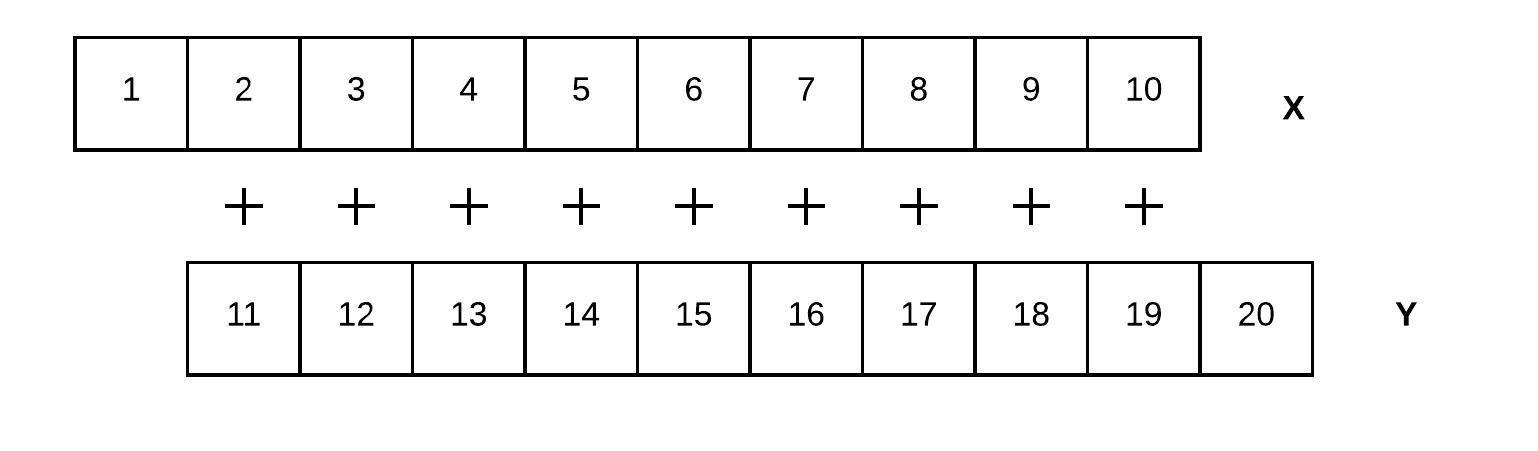
\includegraphics[width=7 cm]{./viz/ext/shiftAndAdd.jpeg}
 
 Note that you are allowed to use only one arithmetic operator
\end{DIY}

\begin{DIY}{Homework}
Given vector X and Y, compute $X^2$ without using the $\wedge$ operator
\end{DIY}

\subsubsection{Vectorizing with Comparison Operators}
\begin{knitrout}
\definecolor{shadecolor}{rgb}{0.969, 0.969, 0.969}\color{fgcolor}\begin{kframe}
\begin{alltt}
\hlstd{X}\hlkwb{<-}\hlkwd{seq}\hlstd{(}\hlnum{1}\hlstd{,}\hlnum{10}\hlstd{)} \hlcom{## generate a sequence of numbers from 1 to 10}
\hlstd{Y}\hlkwb{<-}\hlkwd{seq}\hlstd{(}\hlnum{11}\hlstd{,}\hlnum{20}\hlstd{)} \hlcom{## generate a sequence of numbers from 11 to 20}
\hlstd{X} \hlopt{>} \hlstd{Y}    \hlcom{##check if X is greater than Y}
\end{alltt}
\begin{verbatim}
##  [1] FALSE FALSE FALSE FALSE FALSE FALSE FALSE FALSE FALSE FALSE
\end{verbatim}
\begin{alltt}
\hlstd{Y[}\hlnum{5}\hlstd{]}\hlkwb{<-}\hlstd{X[}\hlnum{5}\hlstd{]} \hlcom{##set the 5th element of Y equal to the 5th element of X}
\hlstd{X} \hlopt{==} \hlstd{Y} \hlcom{##check for equality between X and Y}
\end{alltt}
\begin{verbatim}
##  [1] FALSE FALSE FALSE FALSE  TRUE FALSE FALSE FALSE FALSE FALSE
\end{verbatim}
\end{kframe}
\end{knitrout}

\begin{DIY}{Think}
What is the return type of applying comparison operators on vectors
\end{DIY}

\subsubsection{Are All Values True?}
\begin{knitrout}
\definecolor{shadecolor}{rgb}{0.969, 0.969, 0.969}\color{fgcolor}\begin{kframe}
\begin{alltt}
\hlstd{X}\hlkwb{<-}\hlkwd{seq}\hlstd{(}\hlnum{1}\hlstd{,}\hlnum{10}\hlstd{)} \hlcom{## generate a sequence of numbers from 1 to 10}
\hlstd{Y}\hlkwb{<-}\hlkwd{seq}\hlstd{(}\hlnum{11}\hlstd{,}\hlnum{20}\hlstd{)} \hlcom{## generate a sequence of numbers from 11 to 20}
\hlkwd{all}\hlstd{(Y} \hlopt{>} \hlstd{X)}
\end{alltt}
\begin{verbatim}
## [1] TRUE
\end{verbatim}
\begin{alltt}
\hlstd{Y[}\hlnum{5}\hlstd{]}\hlkwb{<-}\hlstd{X[}\hlnum{5}\hlstd{]} \hlcom{##set the 5th element of Y equal to the 5th element of X}
\hlkwd{all}\hlstd{(Y} \hlopt{==} \hlstd{X)}
\end{alltt}
\begin{verbatim}
## [1] FALSE
\end{verbatim}
\end{kframe}
\end{knitrout}

\subsubsection{Which Values Are True?}
\begin{knitrout}
\definecolor{shadecolor}{rgb}{0.969, 0.969, 0.969}\color{fgcolor}\begin{kframe}
\begin{alltt}
\hlstd{X}\hlkwb{<-}\hlkwd{seq}\hlstd{(}\hlnum{1}\hlstd{,}\hlnum{10}\hlstd{)} \hlcom{## generate a sequence of numbers from 1 to 10}
\hlstd{Y}\hlkwb{<-}\hlkwd{seq}\hlstd{(}\hlnum{11}\hlstd{,}\hlnum{20}\hlstd{)} \hlcom{## generate a sequence of numbers from 11 to 20}
\hlkwd{which}\hlstd{(Y} \hlopt{>} \hlstd{X)}
\end{alltt}
\begin{verbatim}
##  [1]  1  2  3  4  5  6  7  8  9 10
\end{verbatim}
\begin{alltt}
\hlstd{Y[}\hlnum{5}\hlstd{]}\hlkwb{<-}\hlstd{X[}\hlnum{5}\hlstd{]} \hlcom{##set the 5th element of Y equal to the 5th element of X}
\hlkwd{which}\hlstd{(Y} \hlopt{==} \hlstd{X)}
\end{alltt}
\begin{verbatim}
## [1] 5
\end{verbatim}
\begin{alltt}
\hlstd{X[X}\hlopt{==}\hlstd{Y]} \hlcom{##return the element of X that is equal to Y.}
\end{alltt}
\begin{verbatim}
## [1] 5
\end{verbatim}
\end{kframe}
\end{knitrout}

\begin{DIY}{Homework}
Using one arithmetic operation on Y, transform Y in a way such that $all(X==Y)$ returns TRUE
\end{DIY}

\begin{DIY}{Homework}
Using one arithmetic operation on Y, transform Y in a way such that $all(X<Y)$ returns TRUE
\end{DIY}

\begin{DIY}{Homework}
Transform only the values of Y that are even numbers, in such a way that they are all less than X. Then compare them with their corresponding values in X to verify if they are less. Try to do this in as few steps as possible.
\end{DIY}


% !Rnw root = Introduction.Rnw
\newpage
%===============================
%===============================
\section{Data Frames}
%===============================
%==================================  
\subsection{Data sets in R}
%==================================  
\noindent R comes packaged with a list of data sets which can be viewed with the following command: 
\begin{knitrout}
\definecolor{shadecolor}{rgb}{0.969, 0.969, 0.969}\color{fgcolor}\begin{kframe}
\begin{alltt}
\hlkwd{library}\hlstd{(}\hlkwc{help} \hlstd{=} \hlstr{"datasets"}\hlstd{)}
\end{alltt}
\end{kframe}
\end{knitrout}
\noindent These data sets are a great starting point for new comers to try out different R expressions on, and getting your hands dirty. 
%==================================  
\subsection{View a data set}
\subsubsection{The $View()$ function}
%==================================  
\noindent The $View()$ function can be used to see the contents of a data set wherein the argument to the function is the object that contains the data.
\begin{knitrout}
\definecolor{shadecolor}{rgb}{0.969, 0.969, 0.969}\color{fgcolor}\begin{kframe}
\begin{alltt}
\hlkwd{View}\hlstd{(iris)} \hlcom{##see the contents of a data frame}
\end{alltt}
\end{kframe}
\end{knitrout}
%==================================  
\subsection{Type of an Data Frame}
\subsubsection{The $class()$ function}
%==================================  
\noindent We can get the type of an R object by using the $class()$ function. This is synonymous to using the $DESC()$ function in your SQL query  
\begin{knitrout}
\definecolor{shadecolor}{rgb}{0.969, 0.969, 0.969}\color{fgcolor}\begin{kframe}
\begin{alltt}
\hlkwd{class}\hlstd{(iris)} \hlcom{## get the type of a data frame}
\end{alltt}
\begin{verbatim}
## [1] "data.frame"
\end{verbatim}
\end{kframe}
\end{knitrout}
%==================================  
\subsection{Size of a Data Frame}
\subsubsection{The $dim()$ function}
%==================================  
\noindent For objects that have a tabular structure, the $dim()$ function enables us to get the number of rows (observations) and number of columns (attributes)  
\begin{knitrout}
\definecolor{shadecolor}{rgb}{0.969, 0.969, 0.969}\color{fgcolor}\begin{kframe}
\begin{alltt}
\hlkwd{dim}\hlstd{(iris)} \hlcom{##get the dimensions (number of rows,number of columns)}
\end{alltt}
\begin{verbatim}
## [1] 150   5
\end{verbatim}
\end{kframe}
\end{knitrout}
\noindent Now,try:
\begin{knitrout}
\definecolor{shadecolor}{rgb}{0.969, 0.969, 0.969}\color{fgcolor}\begin{kframe}
\begin{alltt}
\hlkwd{class}\hlstd{(}\hlkwd{dim}\hlstd{(iris))} \hlcom{##get the class of the object returned by}
\end{alltt}
\begin{verbatim}
## [1] "integer"
\end{verbatim}
\begin{alltt}
\hlcom{##the call to dim() function}
\end{alltt}
\end{kframe}
\end{knitrout}
\begin{DIY}{Think}
Do you see the difference in result when iris is passed as an argument to $class()$ v/s when $dim(iris)$ is passed as an argument to $class()$. Think about what does the output signify?   
\end{DIY}

\begin{DIY}{Think}
Did you notice how $class()$ takes a data.frame as an argument in one case while takes $dim(iris)$ in another. Relate this observation to the ideas of objects and encapsulation that we have discussed until now.   
\end{DIY}

\begin{DIY}{Homework}
Get only the row count of the data set
\end{DIY}

%==================================  
\subsection{Attribute of a Data Frame}
\subsubsection{The \textbf{\$} operator}
%==================================  
\noindent Attributes of an R object can be accessed by the \textbf{\$} operator. This operator is synonymous to selecting a column in a spreadsheet or a database table.
\begin{knitrout}
\definecolor{shadecolor}{rgb}{0.969, 0.969, 0.969}\color{fgcolor}\begin{kframe}
\begin{alltt}
\hlstd{resut}\hlkwb{<-}\hlstd{iris}\hlopt{$}\hlstd{Sepal.Length} \hlcom{##acessing columns of a data frame}
\end{alltt}
\end{kframe}
\end{knitrout}
%==================================  
\subsection{Create a Histogram}
\subsubsection{The $hist()$ function}
%==================================  
\noindent A histogram which plots the number of occurrences of distinct elements (\textbf{\emph{discrete variables}}) in the attribute or number of occurrences of distinct intervals (\textbf{\emph{continuous variables}}) in the attribute.
\begin{knitrout}
\definecolor{shadecolor}{rgb}{0.969, 0.969, 0.969}\color{fgcolor}\begin{kframe}
\begin{alltt}
\hlkwd{hist}\hlstd{(iris}\hlopt{$}\hlstd{Sepal.Length)} \hlcom{##create a histogram of sepal sength which}
\end{alltt}
\end{kframe}
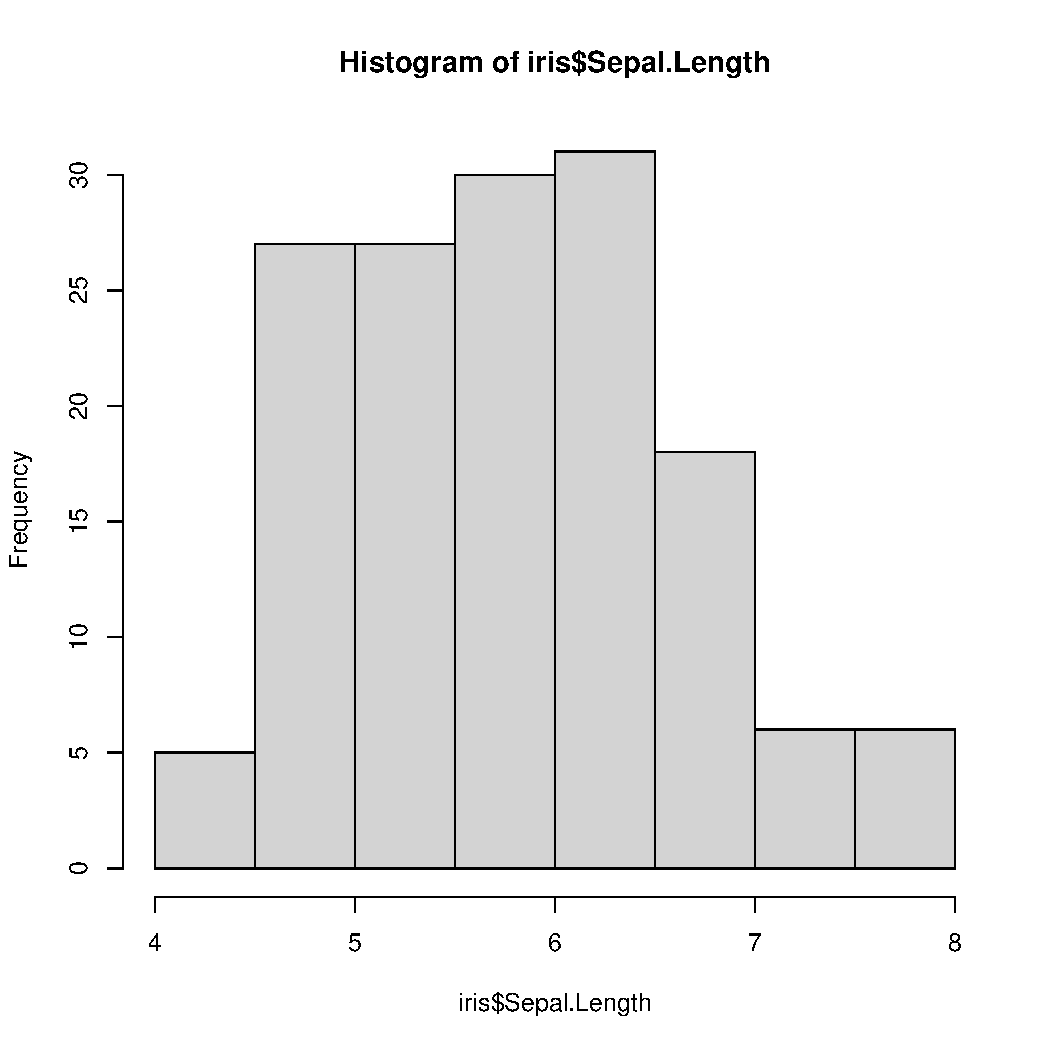
\includegraphics[width=\maxwidth]{figure/hist-1} 
\begin{kframe}\begin{alltt}
\hlcom{##is a vector of the numeric class}
\end{alltt}
\end{kframe}
\end{knitrout}

\begin{DIY}{Think}
Is the argument passed to $hist()$ a \emph{discrete attribute} or a \emph{continuous attribute}? Explain your choice.
\end{DIY}

\begin{DIY}{Think}
Change the histogram plot to show normalized frequencies
\end{DIY}

\begin{DIY}{Homework}
Find the sum of the first 10 and last 10 sepal lengths.
\end{DIY}
%==================================  
\subsection{Create a Scatterplot}
\subsubsection{The $plot()$ function}
%==================================  
\noindent The plot function takes two numeric arrays as arguments and treats each pair of values in the in the arguments as $(X,Y$ coordinates, thereby producing a scatter plot 
\begin{knitrout}
\definecolor{shadecolor}{rgb}{0.969, 0.969, 0.969}\color{fgcolor}\begin{kframe}
\begin{alltt}
\hlkwd{plot}\hlstd{(cars}\hlopt{$}\hlstd{speed,cars}\hlopt{$}\hlstd{dist)} \hlcom{##create a scatter plot with speed on the x axis}
\end{alltt}
\end{kframe}
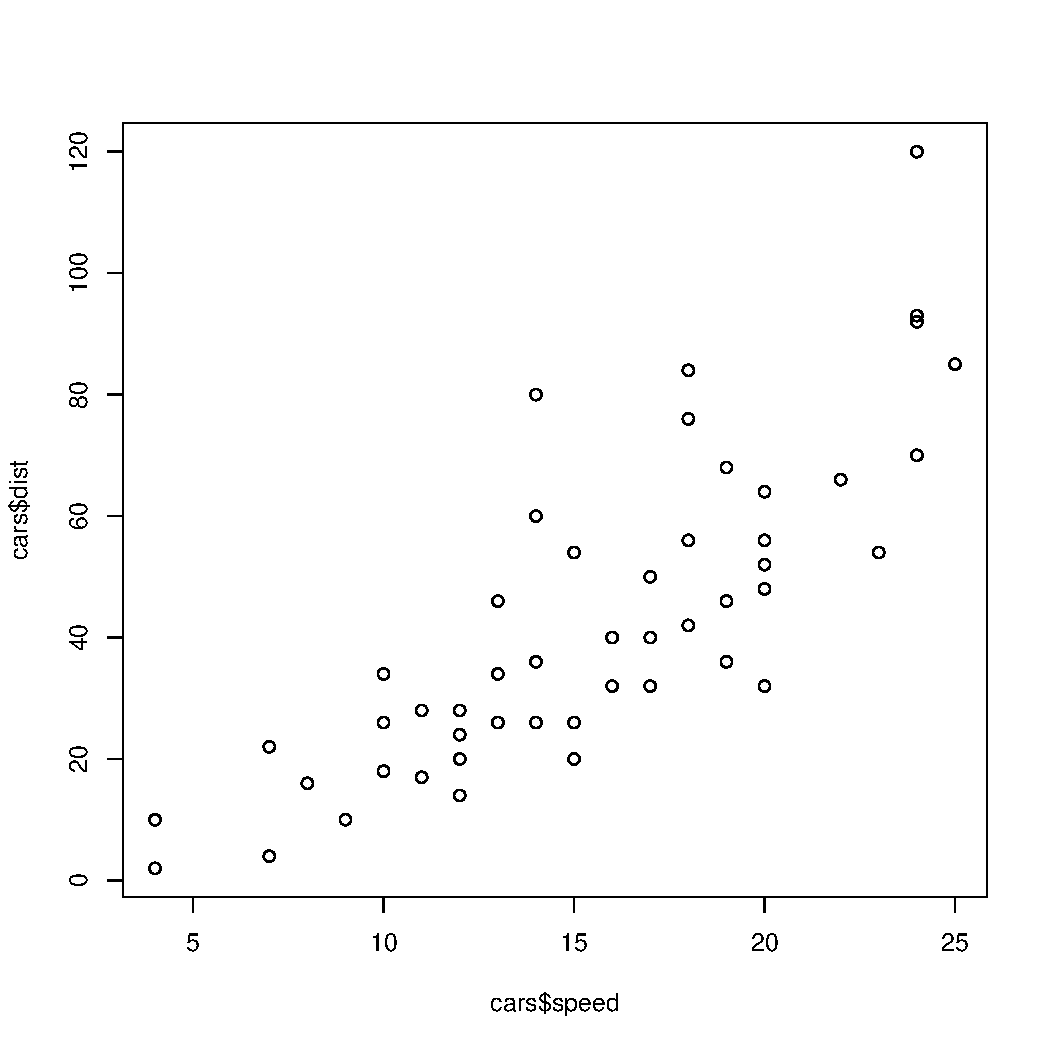
\includegraphics[width=\maxwidth]{figure/plot-1} 
\begin{kframe}\begin{alltt}
\hlcom{## and distance on the y axis}
\end{alltt}
\end{kframe}
\end{knitrout}

\begin{DIY}{Think}
Can you \emph{explain} the plot that you see above?
\end{DIY}

\begin{DIY}{Think}
Change the markers in the plot from circles to crosses. Moreover change the of the markers
\end{DIY}

\begin{DIY}{Think}
What will you get when you pass a data frame with three attributes as an argument to the $plot()$ function
\end{DIY}

%==================================  
\subsection{Create a Data Frame}
%==================================  
\begin{knitrout}
\definecolor{shadecolor}{rgb}{0.969, 0.969, 0.969}\color{fgcolor}\begin{kframe}
\begin{alltt}
\hlstd{X}\hlkwb{<-}\hlkwd{data.frame}\hlstd{(}\hlkwd{c}\hlstd{(}\hlnum{1}\hlstd{,}\hlnum{2}\hlstd{),}\hlkwd{c}\hlstd{(}\hlstr{"apples"}\hlstd{,}\hlstr{"oranges"}\hlstd{),}
              \hlkwd{c}\hlstd{(}\hlnum{TRUE}\hlstd{,}\hlnum{FALSE}\hlstd{))}  \hlcom{##adding data to a data frame wherein }
\hlcom{##each vector represents a column of the deta frame}
\hlstd{X}
\end{alltt}
\begin{verbatim}
##   c.1..2. c..apples....oranges.. c.TRUE..FALSE.
## 1       1                 apples           TRUE
## 2       2                oranges          FALSE
\end{verbatim}
\begin{alltt}
\hlkwd{names}\hlstd{(X)}\hlkwb{<-}\hlkwd{c}\hlstd{(}\hlstr{"id"}\hlstd{,}\hlstr{"fruits"}\hlstd{,}\hlstr{"has_vitaminC"}\hlstd{)} \hlcom{##adding attribute names }
\hlcom{##to the data frame}
\hlstd{X}
\end{alltt}
\begin{verbatim}
##   id  fruits has_vitaminC
## 1  1  apples         TRUE
## 2  2 oranges        FALSE
\end{verbatim}
\begin{alltt}
\hlstd{X}\hlopt{$}\hlstd{fruits}
\end{alltt}
\begin{verbatim}
## [1] apples  oranges
## Levels: apples oranges
\end{verbatim}
\end{kframe}
\end{knitrout}

\begin{DIY}{Think}
The output for the last expression shows that the attribute fruits has levels. What does this mean?
\end{DIY}

\begin{DIY}{Homework}
Pick a data set from the list of available data sets and \emph{explore it} using the \emph{R expressions} you have just learnt.
\end{DIY}

\begin{DIY}{Homework}
Create a data frame for the example shown in section \ref{sec:GeomOfData} and generate the plot that was shown in the same section.
\end{DIY}


% !Rnw root = UsingR.Rnw
\newpage
%===============================
\section{Input/Output with External Sources}
%===============================
\begin{HIGHLIGHT}
\par\noindent{
Reading in data from files like ``\textbf{.txt}'',``\textbf{.csv}'' and ``\textbf{.xls}'' into the R environment has been greatly simplified by RStudio. Just goto  Environment tab $->$ Import Dataset  and select the file type from which you want to import the data (for \emph{.txt} and  \emph{.csv} files choose the ``From CSV...'' option while for excel sheets choose ``From Excel..'' option). A new window will open up with a set of options that will guide you to import your data in R.        
}
R also provides a set of functions for reading and writing data. An inquisitive reader can read about them in \textcolor{cyan}{\url{https://www.datacamp.com/community/tutorials/r-tutorial-read-excel-into-r}}
\end{HIGHLIGHT}

\begin{DIY}{Think}
Though RStudio has simplified the process of reading in data by providing a GUI, it hasn't provided any mechanism for writing data out of the R environment. What do you think this is the reason for this?  
\end{DIY}

\begin{DIY}{Homework}
Do the following
\begin{enumerate}
  \item Remove the headers from exercise1.csv and try importing it into the R environment. What do you observe?
  \item Replace exercise1.csv as exercise1.tsv (i.e change the delimiter between attributes from comma to tab) and try importing it into the R environment.
\end{enumerate}
\end{DIY}
%===============================
\subsection{IO with RDBMS}
%===============================
%=============================
\begin{figure}[ht]
 \centering
    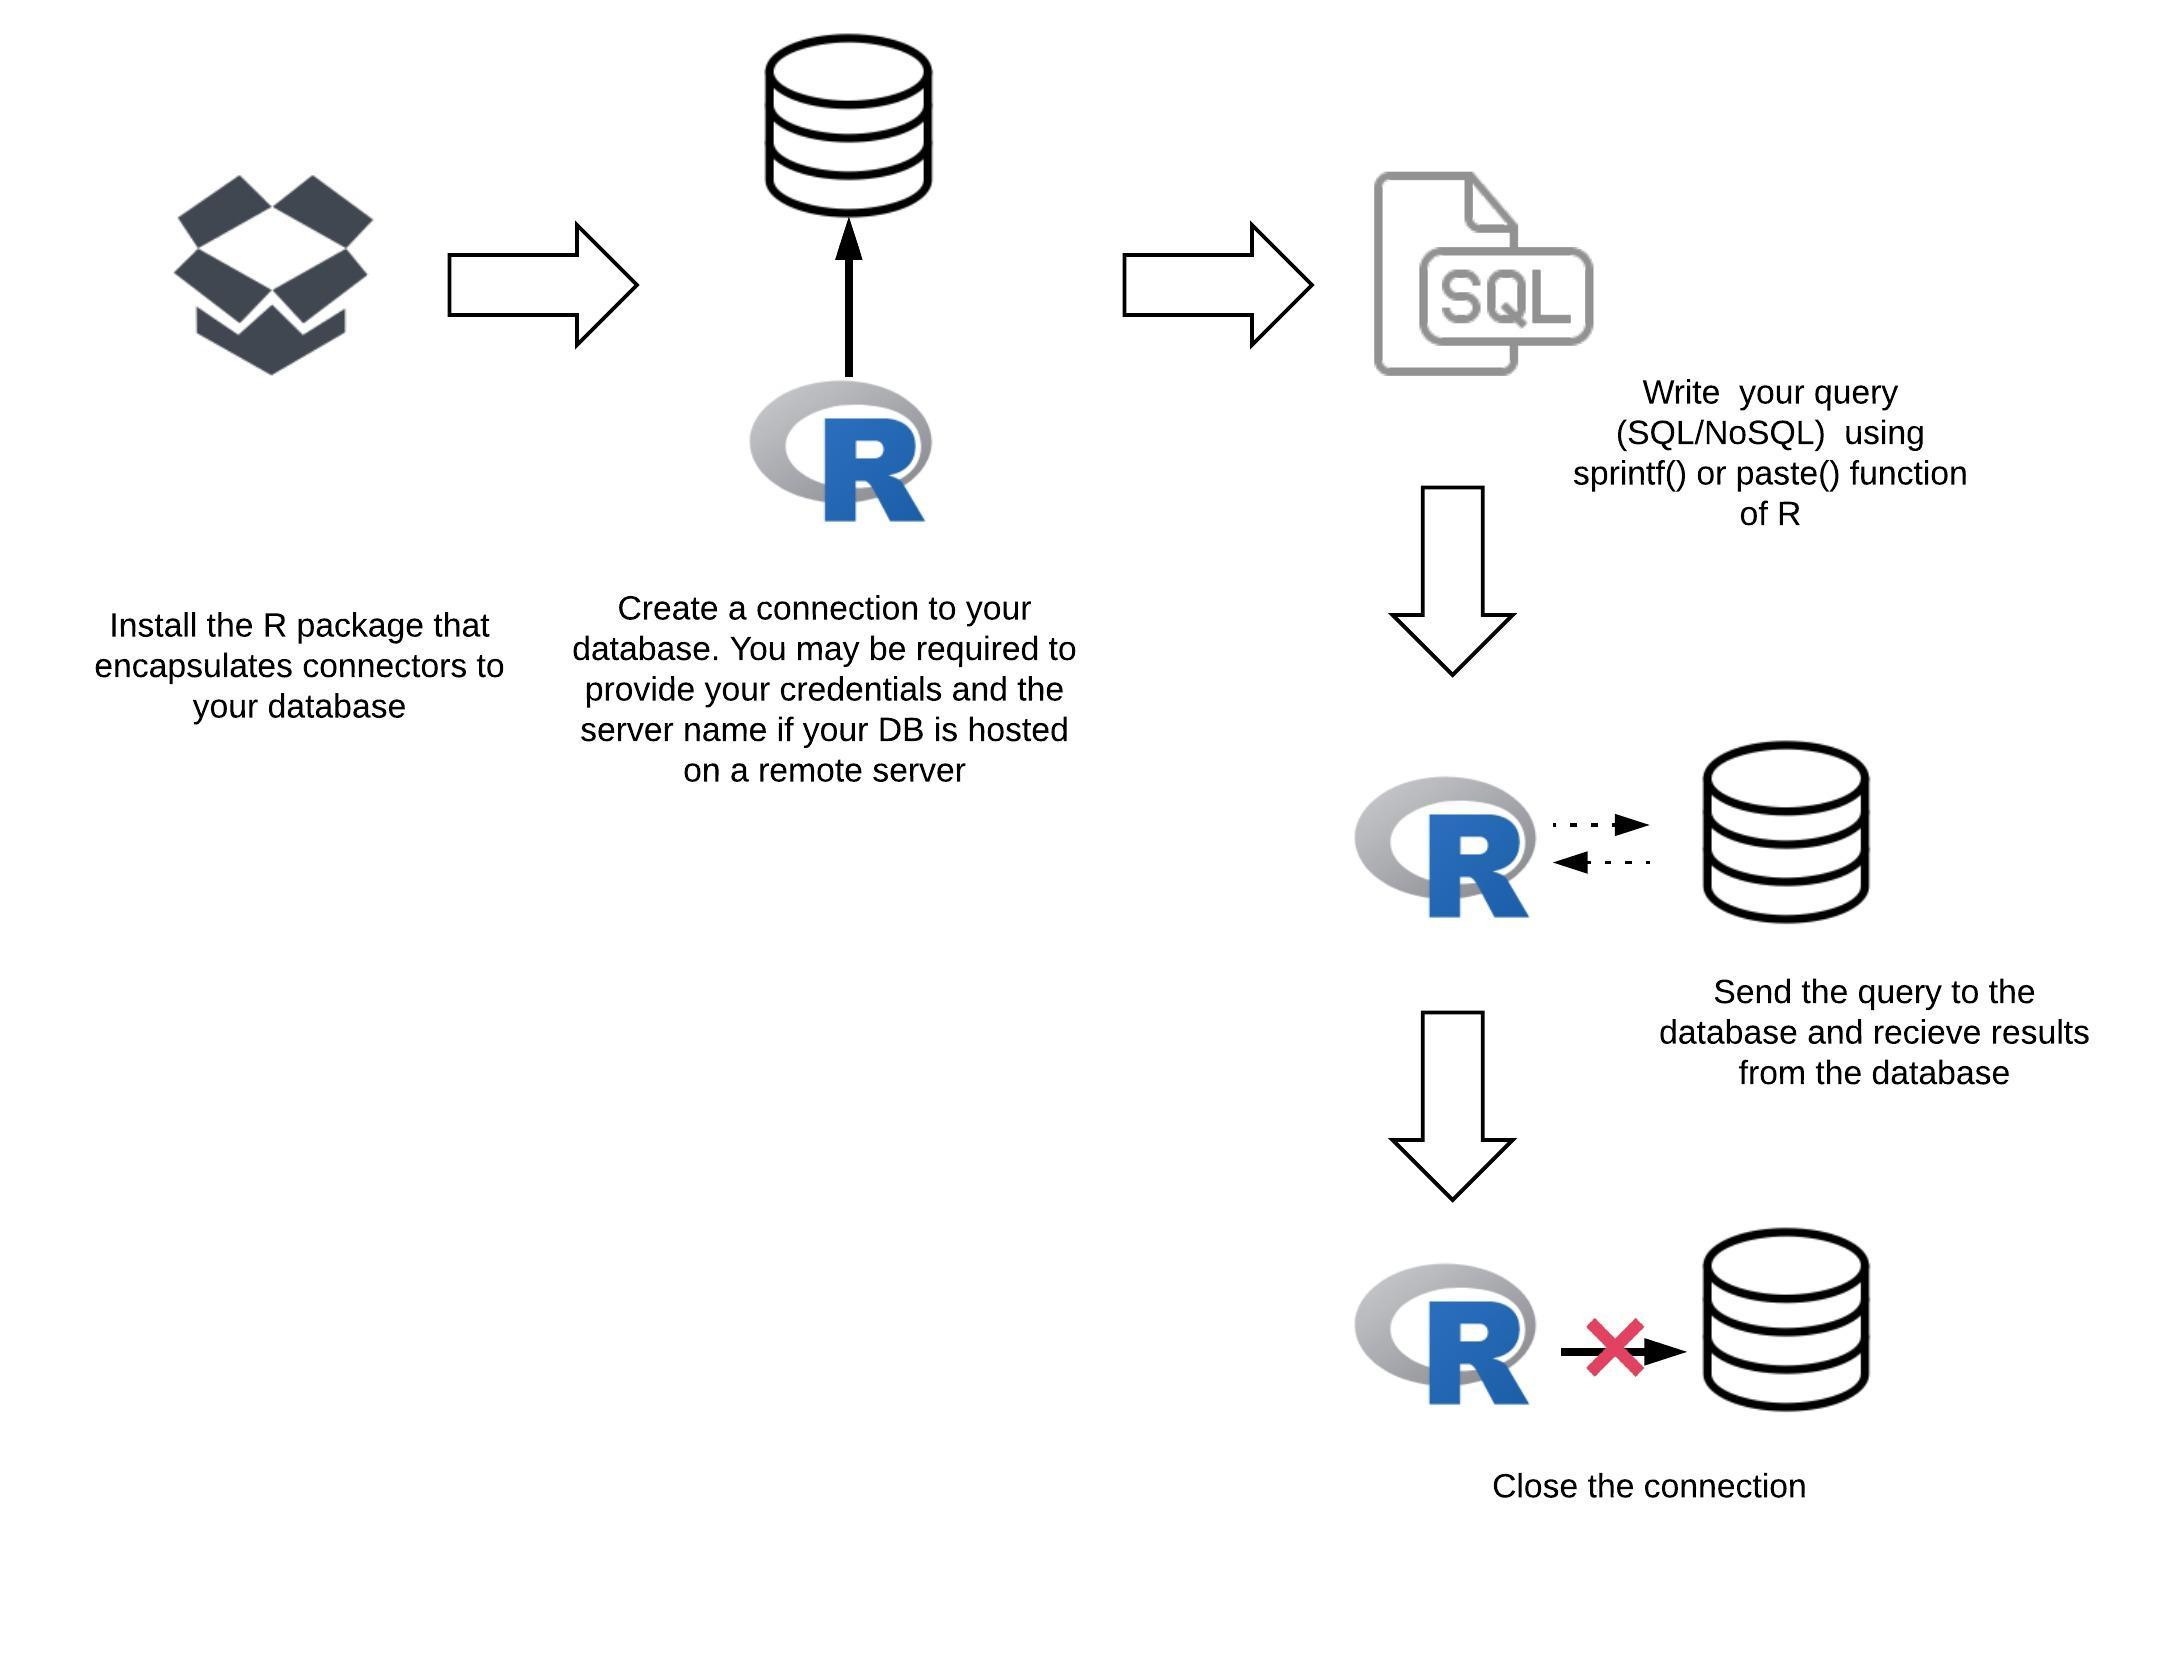
\includegraphics[width = 15 cm]{./viz/ext/IO_R_RDBMS.jpeg}
\end{figure}
\begin{HIGHLIGHT}
A large number of different databases exist in the market and each of them has is its own way of setting up and managing connections with client applications. These low level connection details are encapsulated by R packages and the user only has to be aware of an abstract view as shown in the schematic. Details of R packages for connecting to some of the popular databases can be found in the following links:
\begin{itemize}
  \item How to Connect to an Oracle Database:
  
  \textcolor{cyan}{\url {http://rprogramming.net/connect-to-database-in-r/}}
  \item How to Connect to a MySQL Database:
  
  \textcolor{cyan}{\url {https://www.r-bloggers.com/mysql-and-r/}}
  \item How to Connect to MongoDB: 
  
  \textcolor{cyan}{\url {https://www.r-bloggers.com/r-and-mongodb/}}
\end{itemize}
\end{HIGHLIGHT}

As, shown in the schematic, SQL queries can be constructed with the $sprintf()$ and $paste()$ function. We give a few examples here:
\begin{knitrout}
\definecolor{shadecolor}{rgb}{0.969, 0.969, 0.969}\color{fgcolor}\begin{kframe}
\begin{alltt}
\hlkwd{sprintf}\hlstd{(}\hlstr{"select * from names where name in (%s)"}\hlstd{,}
        \hlkwd{paste}\hlstd{(}\hlkwd{c}\hlstd{(}\hlstr{"'Andrew"}\hlstd{,}\hlstr{"John"}\hlstd{,}\hlstr{"Jane'"}\hlstd{),}\hlkwc{collapse}\hlstd{=}\hlstr{"','"}\hlstd{)}
       \hlstd{)}
\end{alltt}
\begin{verbatim}
## [1] "select * from names where name in ('Andrew','John','Jane')"
\end{verbatim}
\begin{alltt}
\hlkwd{sprintf}\hlstd{(}\hlstr{"insert into networks (id, name) values (%d, '%s');"}\hlstd{,}
                    \hlnum{11}\hlstd{,} \hlstr{"John"}
        \hlstd{)}
\end{alltt}
\begin{verbatim}
## [1] "insert into networks (id, name) values (11, 'John');"
\end{verbatim}
\end{kframe}
\end{knitrout}

\begin{DIY}{Warning}
Yes, it is indeed complicated to write queries in R as compared to writing them in a SQL editor. But the idea is to realize, as a user that one should do complicated aggregations and transformation of the data either solely in the database and store it back in tables where R can query from or within R itself (after having imported the data) but \textbf{NEVER} at the interface level. \emph{Complicated interfaces lead to unmanageable software}.When you have large amounts of data, trying to read in all the data of the database into R and then doing the data aggregation and transformation in R is also \textbf{NOT} a good idea as it creates a lot of dependency on the connector between R and the database which may have its own limitations based on how it has been implemented.  
\end{DIY}

\cleardoublepage
\thispagestyle{empty}
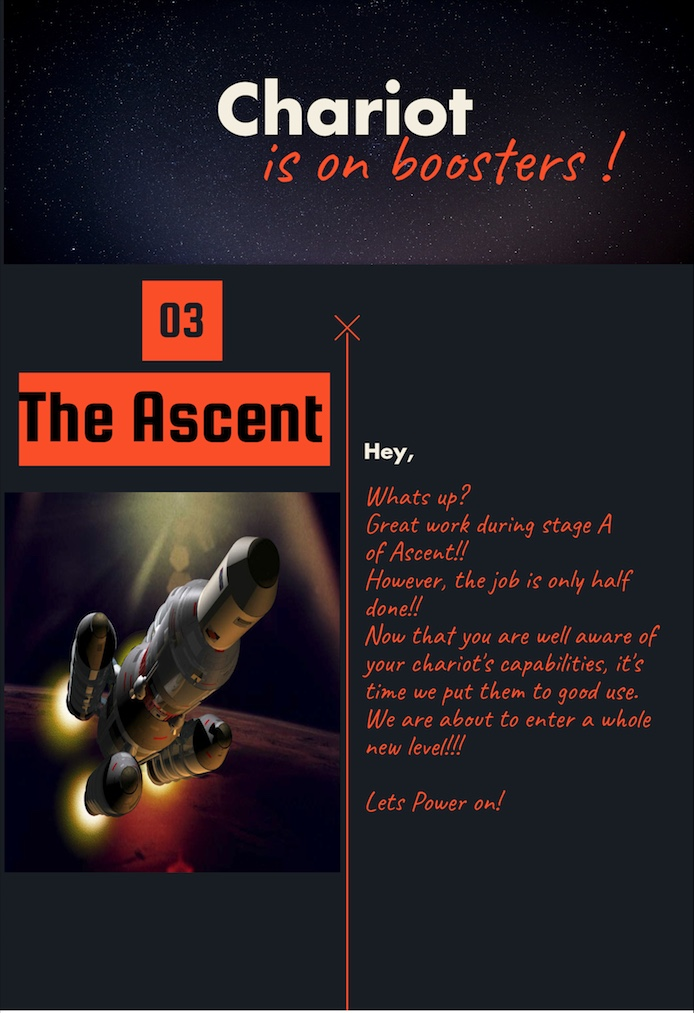
\includegraphics[width = 16 cm]{./viz/ext/Ascent_B.jpeg}

%=======================================
\chapter{The Ascent - PART B}
%=======================================

% !Rnw root = main.Rnw


% !Rnw root = Introduction.Rnw
%===============================
\section{The Dataset}
%===============================
\textbf{Its time to get real!!}. We give you the \textbf{``Yelp Open Dataset''} . 
For the rest of our journey, we will be presenting different data manipulation, visualization and modelling techniques using this data set as our example. The idea is to get you acquainted with  typically large, and noisy data sets as is prevalent in today's world and to show you how to explore these data sets using R. The data set has been provided to you as set of 11 files, along with this reader. The inter-relation between the attributes can be found at the end of this chapter. Further details of the data set can be found in \textcolor{cyan}{\url{https://www.yelp.com/dataset}} 

\begin{figure}[ht]
 \centering
    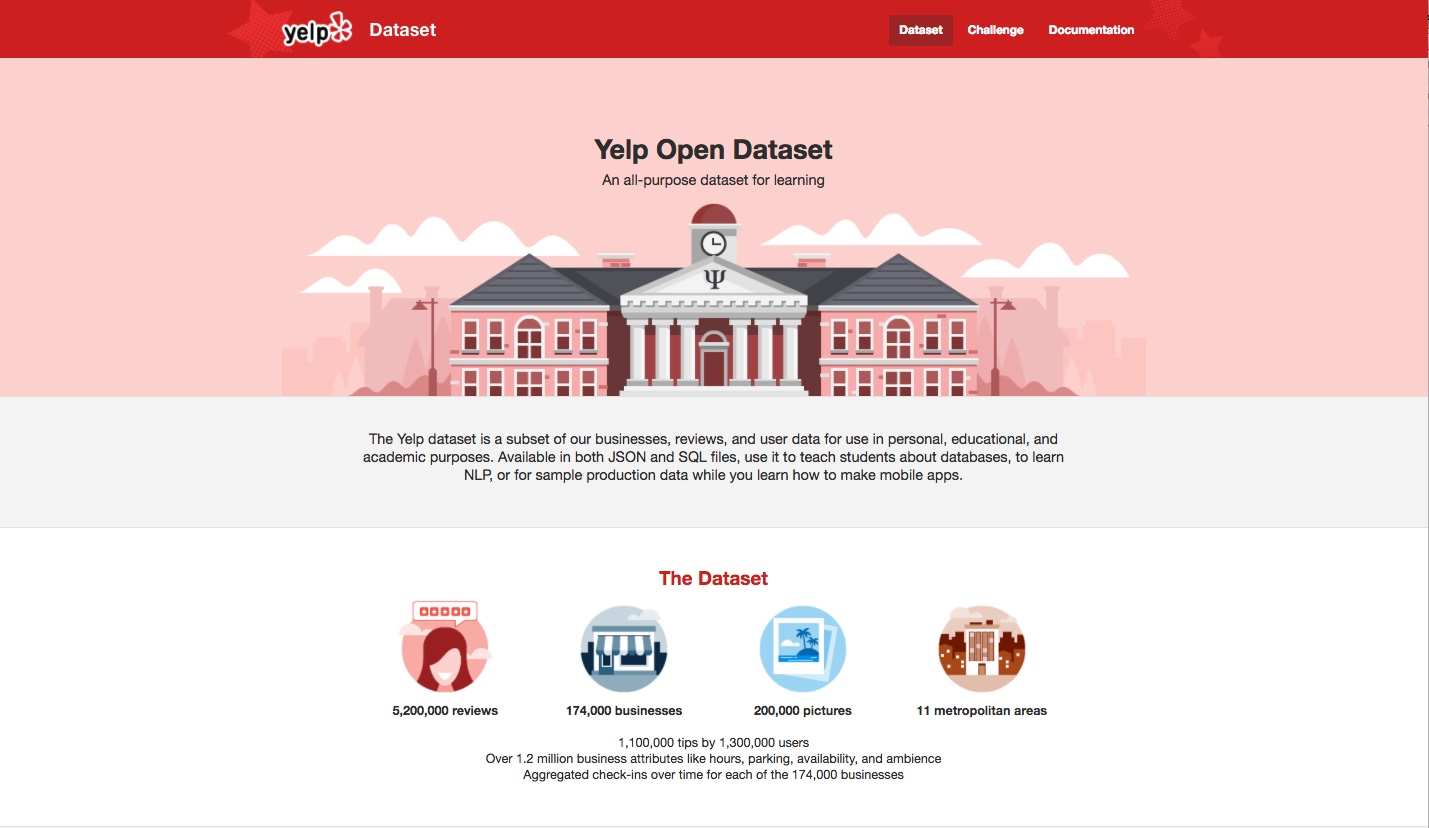
\includegraphics[ height=11cm,width = 15 cm]{./viz/ext/theYelpDataset.jpeg}
\end{figure}



% !Rnw root = Introduction.Rnw
%===============================
\section{Data Wrangling}
%===============================

\begin{HIGHLIGHT}
\par\noindent{
\noindent \textbf{\emph{Data Wrangling}} sometimes referred to as data munging, is the process of transforming and mapping data from its raw form to a form that is suitable for analysis.
Exploring data for new insights is a gradual, iterative process. Occasionally we get a sudden insight, but for the most part we try something, look at the results, reflect a bit, and then try something slightly different.
}
\end{HIGHLIGHT}

\noindent In this section, we will learn about ways to  \textbf{(a)} Clean \textbf{(b)} Transform and \textbf{(c)} Aggregate data. 
Therefore, we will formulate different questions that we wish to ask on the data and write R expressions that will enable us to answer those questions.

\subsection{The \textbf{\emph{business}} dataset}

\noindent Import the file \emph{\textbf{business.csv}} into your R environment. 


\subsubsection{Dimension and Attributes}
\noindent \textbf{\underline{Question}}: What is the size of the data?
\begin{knitrout}
\definecolor{shadecolor}{rgb}{0.969, 0.969, 0.969}\color{fgcolor}\begin{kframe}
\begin{alltt}
\hlkwd{dim}\hlstd{(business)}
\end{alltt}
\begin{verbatim}
## [1] 156639     12
\end{verbatim}
\begin{alltt}
\hlcom{##get the dimension of the data}
\end{alltt}
\end{kframe}
\end{knitrout}

\noindent \textbf{\underline{Question}}: What are the attributes?
\begin{knitrout}
\definecolor{shadecolor}{rgb}{0.969, 0.969, 0.969}\color{fgcolor}\begin{kframe}
\begin{alltt}
\hlkwd{colnames}\hlstd{(business)}
\end{alltt}
\begin{verbatim}
##  [1] "id"           "name"         "neighborhood" "address"     
##  [5] "city"         "state"        "postal_code"  "latitude"    
##  [9] "longitude"    "stars"        "review_count" "is_open"
\end{verbatim}
\begin{alltt}
\hlcom{##get the attributes of the data}
\end{alltt}
\end{kframe}
\end{knitrout}

\newpage
\subsubsection{Uni-variate Distribution}
\noindent \textbf{\underline{Question}}: What is the distribution of ratings in the data?
\begin{knitrout}
\definecolor{shadecolor}{rgb}{0.969, 0.969, 0.969}\color{fgcolor}\begin{kframe}
\begin{alltt}
\hlkwd{boxplot}\hlstd{(business}\hlopt{$}\hlstd{stars,}\hlkwc{main} \hlstd{=} \hlstr{"Distribution of Ratings"}\hlstd{)}
\end{alltt}
\end{kframe}
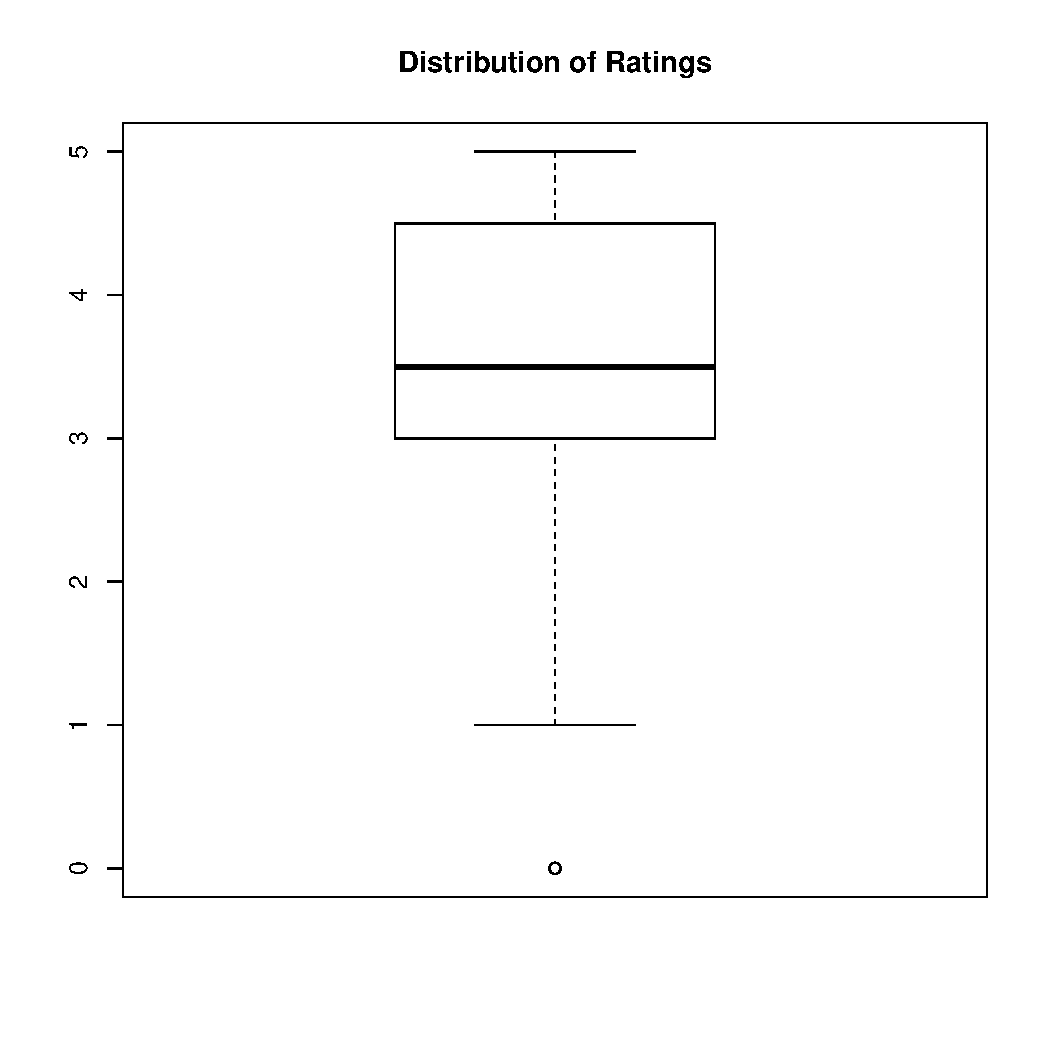
\includegraphics[width=\maxwidth]{figure/boxplotStars-1} 

\end{knitrout}

\begin{DIY}{Think}
\noindent Explain the plot
\end{DIY}

\begin{DIY}{Homework}
\noindent What is the distribution of review count in the data?
\end{DIY}

\newpage
\subsubsection{Sorting and Selection}
\noindent \textbf{\underline{Question}}: Which are the top 10 business by rating? 
\begin{knitrout}
\definecolor{shadecolor}{rgb}{0.969, 0.969, 0.969}\color{fgcolor}\begin{kframe}
\begin{alltt}
\hlkwd{head}\hlstd{(business[}\hlkwd{order}\hlstd{(business}\hlopt{$}\hlstd{stars,}
                    \hlkwc{decreasing} \hlstd{=} \hlnum{TRUE}
                    \hlstd{),}
              \hlkwd{c}\hlstd{(}\hlstr{"name"}\hlstd{,}\hlstr{"state"}\hlstd{,}\hlstr{"stars"}\hlstd{)}
              \hlstd{],}
     \hlkwc{n}\hlstd{=}\hlnum{10}\hlstd{)}
\hlcom{## sort the data by number of  stars and get the top 10 businesses}
\end{alltt}
\end{kframe}
\end{knitrout}

\begin{DIY}{Homework}
\noindent Which are the bottom 10 businesses by review count?
\end{DIY}

\subsubsection{Aggregation}
\noindent \textbf{\underline{Question}}: What is the number of business entities per state? 
\begin{knitrout}
\definecolor{shadecolor}{rgb}{0.969, 0.969, 0.969}\color{fgcolor}\begin{kframe}
\begin{alltt}
\hlstd{countPerState} \hlkwb{<-} \hlkwd{aggregate}\hlstd{(business}\hlopt{$}\hlstd{state,}
                           \hlkwc{by}\hlstd{=}\hlkwd{list}\hlstd{(business}\hlopt{$}\hlstd{state),}
                           \hlkwc{FUN}\hlstd{=length}
                           \hlstd{)}
\hlkwd{names}\hlstd{(countPerState)}\hlkwb{<-}\hlkwd{c}\hlstd{(}\hlstr{"state"}\hlstd{,}\hlstr{"count"}\hlstd{)}
\hlkwd{View}\hlstd{(countPerState)}
\hlcom{##count number of occurences of businesses in each state  }
\end{alltt}
\end{kframe}
\end{knitrout}


\begin{DIY}{Homework}
\noindent Read the help manual for the \emph{aggregate()} function.
\end{DIY}

\begin{DIY}{Think}
\noindent \begin{itemize}
  \item Why have we passed a \emph{list()} to the \textbf{by} argument? 
  \item What do you get if you just set $by = business\$state$?
\end{itemize}
\end{DIY}

\begin{DIY}{Warning}
\noindent Take a close look at the values in the \textbf{countPerState\$state} column. Do you notice any irregularities?
\end{DIY}

\newpage
\subsubsection{Filtering}
\noindent \textbf{\underline{Question}}: How can we filter out incorrect values? 
\begin{knitrout}
\definecolor{shadecolor}{rgb}{0.969, 0.969, 0.969}\color{fgcolor}\begin{kframe}
\begin{alltt}
\hlkwd{View}\hlstd{(countPerState[}\hlkwd{is.na}\hlstd{(}
                         \hlkwd{as.numeric}\hlstd{(countPerState}\hlopt{$}\hlstd{state)}
                         \hlstd{),}
                   \hlstd{]}
     \hlstd{)}
\hlcom{##filter out the entries that are of type "numeric" }
\end{alltt}
\end{kframe}
\end{knitrout}

\begin{DIY}{Think}
\noindent Explain how are we taking advantage of coercion in the above expression.
\end{DIY}

\begin{DIY}{Homework}
\noindent When we count the number of hotels per state, we see that some states are labelled as 'C'. Find the list of all businesses that belong to this state
\end{DIY}

\begin{DIY}{Homework}
\noindent The bounding box of United States in terms of (lat,lon) is (-125.0011, 24.9493) and (-66.9326, 49.5904). Find all
businesses that are located in US. Moreover, find which state in US has the highest number of 5 star businesses.
\end{DIY}

\newpage
\subsubsection{Bi-variate Distribution}
\noindent \textbf{\underline{Question}}: What is the distribution of open v/s closed business? 
\begin{knitrout}
\definecolor{shadecolor}{rgb}{0.969, 0.969, 0.969}\color{fgcolor}\begin{kframe}
\begin{alltt}
\hlkwd{table}\hlstd{(business}\hlopt{$}\hlstd{is_open)}
\hlcom{## get frequency of open v/s closed businesses }
\end{alltt}
\end{kframe}
\end{knitrout}

\begin{DIY}{Homework}
\noindent Refer to \textcolor{cyan}{\url{https://www.statmethods.net/graphs/pie.html}} and generate the pie chart as shown below
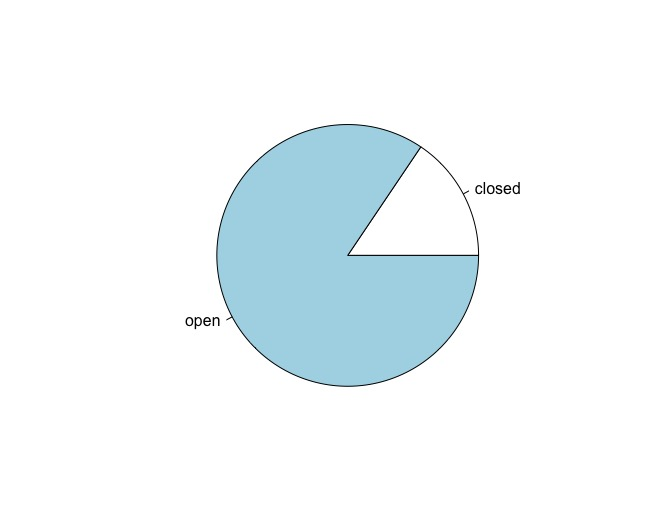
\includegraphics[width=9 cm]{./viz/ext/pieChartBusinessStatus.jpeg}
\end{DIY}


\begin{DIY}{Homework}
\noindent Refer to \textcolor{cyan}{\url{https://www.statmethods.net/graphs/boxplot.html}} and generate the boxplot as shown below. Moreover explain the plot
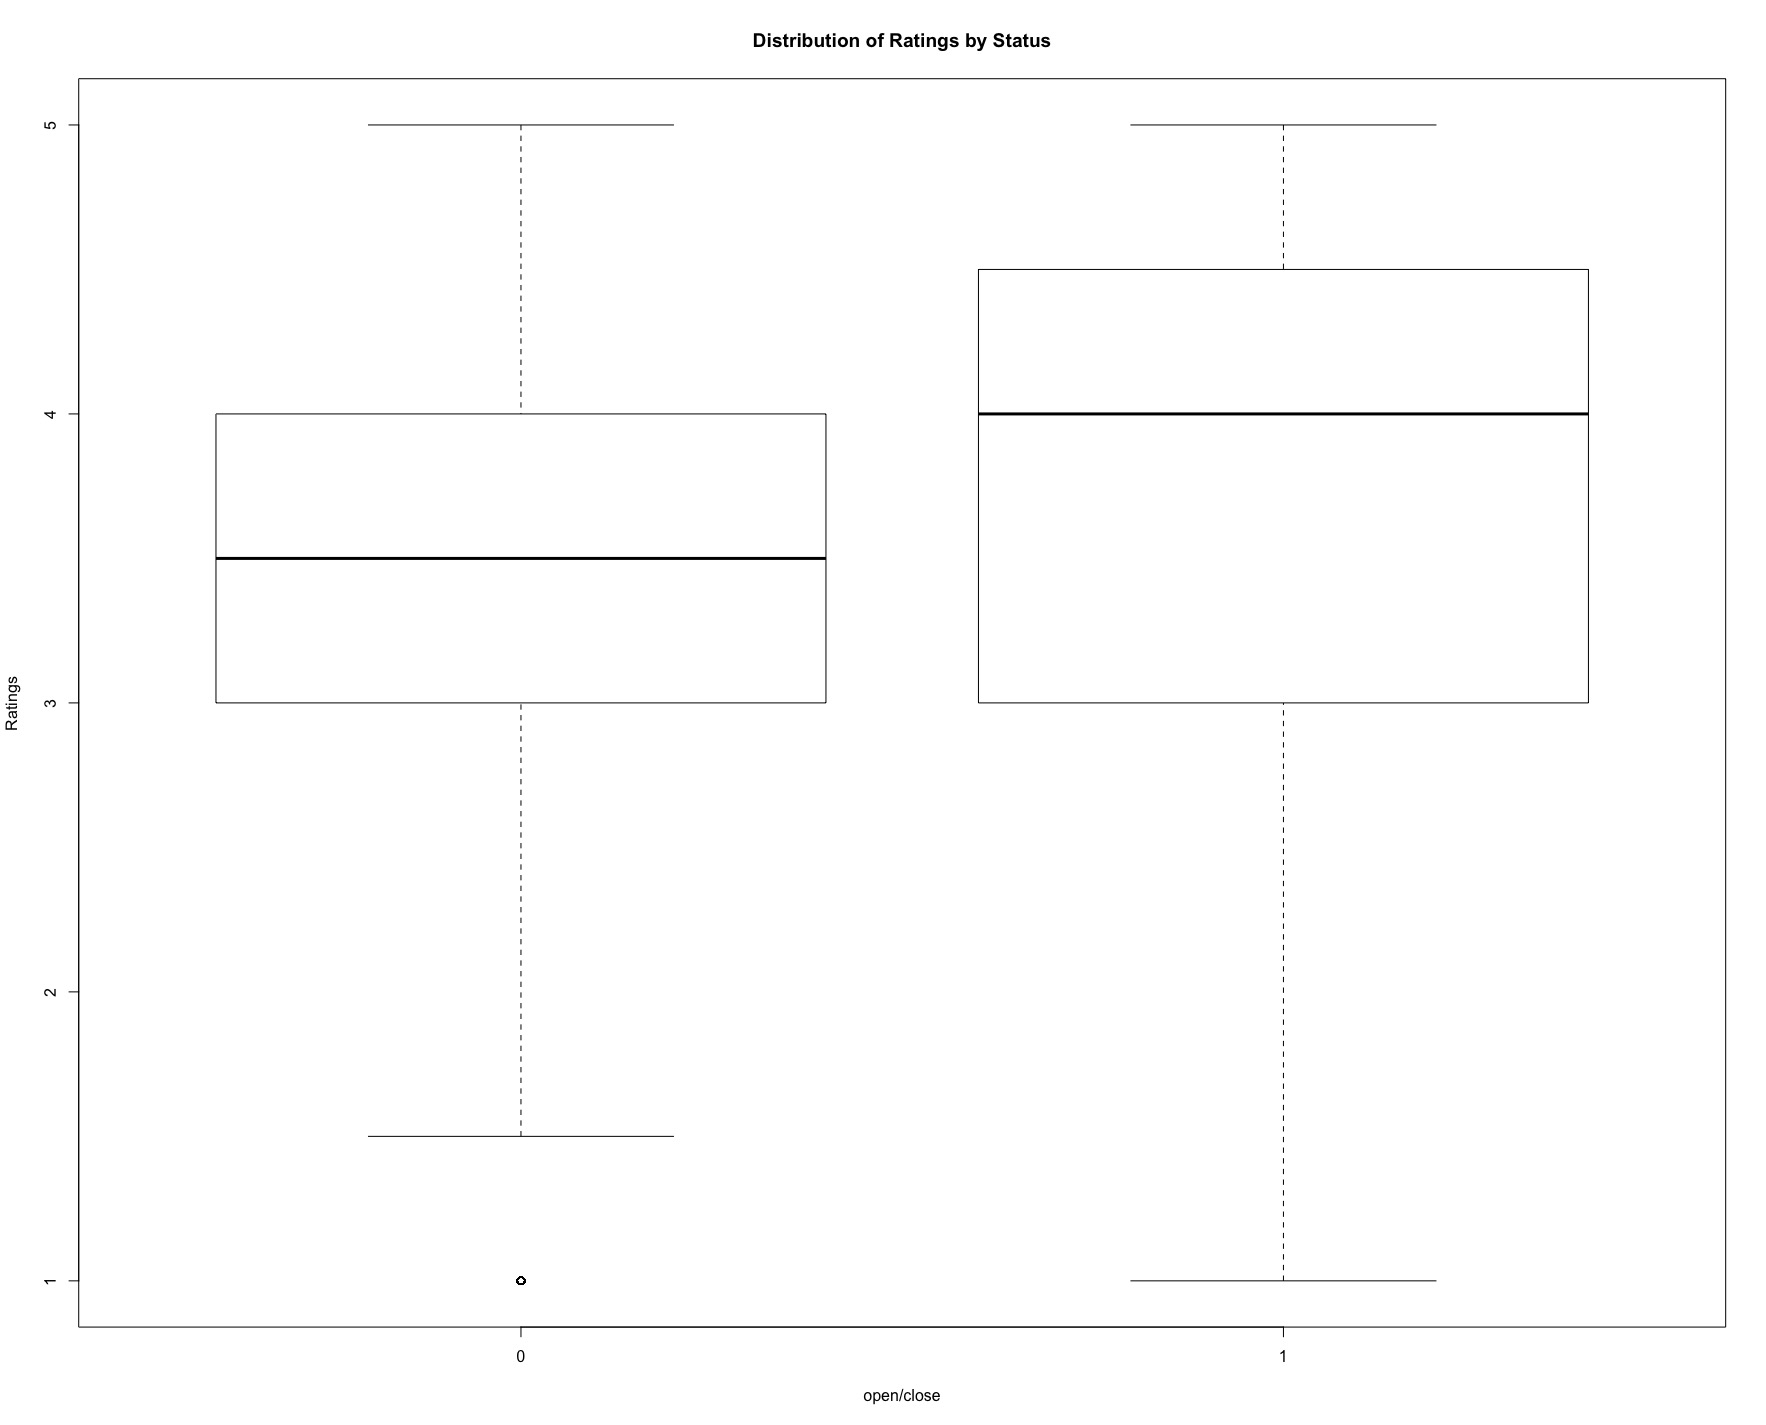
\includegraphics[width=12 cm]{./viz/ext/BoxPlot_Ratings_OpenStatus.jpeg}
\end{DIY}

\newpage
\subsubsection{Relationship among Attributes}
\noindent \textbf{\underline{Question}}: Does there exist a relationship between ratings and number of reviews?
\begin{knitrout}
\definecolor{shadecolor}{rgb}{0.969, 0.969, 0.969}\color{fgcolor}\begin{kframe}
\begin{alltt}
\hlkwd{plot}\hlstd{(business}\hlopt{$}\hlstd{review_count,business}\hlopt{$}\hlstd{stars,}
      \hlkwc{main} \hlstd{=} \hlstr{"Relation b/w review count and rating"}\hlstd{,}
     \hlkwc{xlab} \hlstd{=} \hlstr{"review_count"}\hlstd{,} \hlkwc{ylab} \hlstd{=} \hlstr{"rating"}\hlstd{)}
\end{alltt}
\end{kframe}
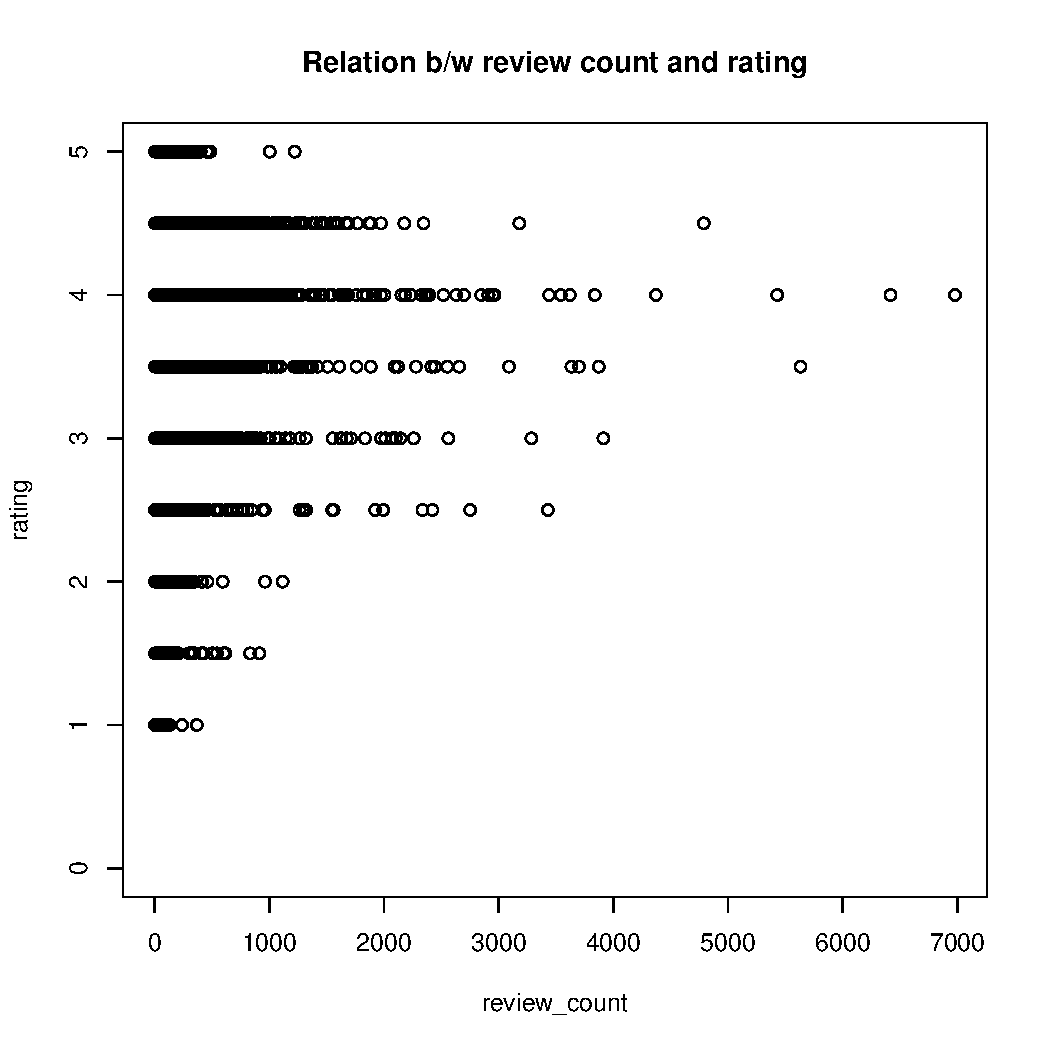
\includegraphics[width=\maxwidth]{figure/corr_Review_Stars-1} 
\begin{kframe}\begin{alltt}
\hlcom{##scatterplot of review count and ratings}
\end{alltt}
\end{kframe}
\end{knitrout}

\begin{DIY}{Think}
\noindent Explain the plot
\end{DIY}

\begin{DIY}{Homework}
\noindent Generate the scatter-plot that plots the relationship between review count and ratings for all open businesses and has number of reviews $\leq$ 1000.
\end{DIY}

\newpage
\subsection{The \textbf{\emph{category}} dataset}
\noindent Import the file \emph{\textbf{category.csv}} into your R environment.  


\subsubsection{Dimension and Attributes}
\noindent \textbf{\underline{Question}}: What is the dimension of the data and what are the various attributes?
\begin{knitrout}
\definecolor{shadecolor}{rgb}{0.969, 0.969, 0.969}\color{fgcolor}\begin{kframe}
\begin{alltt}
\hlkwd{dim}\hlstd{(category)}
\end{alltt}
\begin{verbatim}
## [1] 590290      2
\end{verbatim}
\begin{alltt}
\hlcom{##get dimension of the data}
\hlkwd{colnames}\hlstd{(category)}
\end{alltt}
\begin{verbatim}
## [1] "business_id" "category"
\end{verbatim}
\begin{alltt}
\hlcom{##get attributes of the data}
\end{alltt}
\end{kframe}
\end{knitrout}

\subsubsection{Sorting and Selection}
\noindent \textbf{\underline{Question}}: Which are the 10 most frequent categories?  
\begin{knitrout}
\definecolor{shadecolor}{rgb}{0.969, 0.969, 0.969}\color{fgcolor}\begin{kframe}
\begin{alltt}
\hlstd{countPerCategory} \hlkwb{<-} \hlkwd{aggregate}\hlstd{(category}\hlopt{$}\hlstd{category,}
                              \hlkwc{by}\hlstd{=}\hlkwd{list}\hlstd{(category}\hlopt{$}\hlstd{category),}
                              \hlstd{length}
                             \hlstd{)}
\hlcom{##count the number of occurence of each category}
\hlkwd{names}\hlstd{(countPerCategory)} \hlkwb{<-} \hlkwd{c}\hlstd{(}\hlstr{"category"}\hlstd{,}\hlstr{"count"}\hlstd{)}

\hlstd{top10Categories}\hlkwb{<-}\hlkwd{head}\hlstd{(countPerCategory[}
                            \hlkwd{order}\hlstd{(countPerCategory}\hlopt{$}\hlstd{count,}
                                  \hlkwc{decreasing} \hlstd{=} \hlnum{TRUE}
                                  \hlstd{),}
                          \hlstd{],}
         \hlkwc{n}\hlstd{=}\hlnum{10}
     \hlstd{)}
\hlcom{##sort the frequency data frame in descending order}
\hlcom{##and list the top 10}
\hlstd{top10Categories}
\end{alltt}
\end{kframe}
\end{knitrout}

\noindent \textbf{\underline{Question}}: Which business belong to the 10 most frequent categories?  
\begin{knitrout}
\definecolor{shadecolor}{rgb}{0.969, 0.969, 0.969}\color{fgcolor}\begin{kframe}
\begin{alltt}
\hlstd{businesses_top10Categories} \hlkwb{<-} \hlstd{category[category}\hlopt{$}\hlstd{category} \hlopt
                                         \hlstd{top10Categories[,}\hlnum{1}\hlstd{],]}
\hlcom{##list all entries in the category file that }
\hlcom{#belong to one of the top 10 categories}
\end{alltt}
\end{kframe}
\end{knitrout}

\begin{DIY}{Think}
\noindent How would you check if the filtering criteria applied in the last step returns the correct result
\end{DIY}

\subsubsection{Distribution of the Data}
\noindent \textbf{\underline{Question}}: Are businesses assigned to multiple categories? How many such businesses exist?
\begin{knitrout}
\definecolor{shadecolor}{rgb}{0.969, 0.969, 0.969}\color{fgcolor}\begin{kframe}
\begin{alltt}
\hlstd{businessIdFreq} \hlkwb{<-} \hlkwd{table}\hlstd{(category}\hlopt{$}\hlstd{business_id)}
\hlcom{##get number of categories each business has been assigned to}
\hlkwd{length}\hlstd{(businessIdFreq} \hlopt{>} \hlnum{0}\hlstd{)} \hlopt{>} \hlnum{0}
\end{alltt}
\begin{verbatim}
## [1] TRUE
\end{verbatim}
\begin{alltt}
\hlcom{##check if there are businesses assigned to multiple categories}
\hlkwd{plot}\hlstd{(businessIdFreq[}\hlkwd{order}\hlstd{(}
                          \hlstd{businessIdFreq,}
                          \hlkwc{decreasing} \hlstd{=} \hlnum{TRUE}
                          \hlstd{)}
                    \hlstd{],}
     \hlkwc{xlab} \hlstd{=} \hlstr{"Businesses"}\hlstd{,}
     \hlkwc{ylab}\hlstd{=}\hlstr{"Number of Assigned Categories"}\hlstd{,}
     \hlkwc{main} \hlstd{=} \hlstr{"Distribution of category assignment of businesses"}\hlstd{,}
     \hlkwc{xaxt} \hlstd{=} \hlstr{'n'}\hlstd{)}
\end{alltt}
\end{kframe}
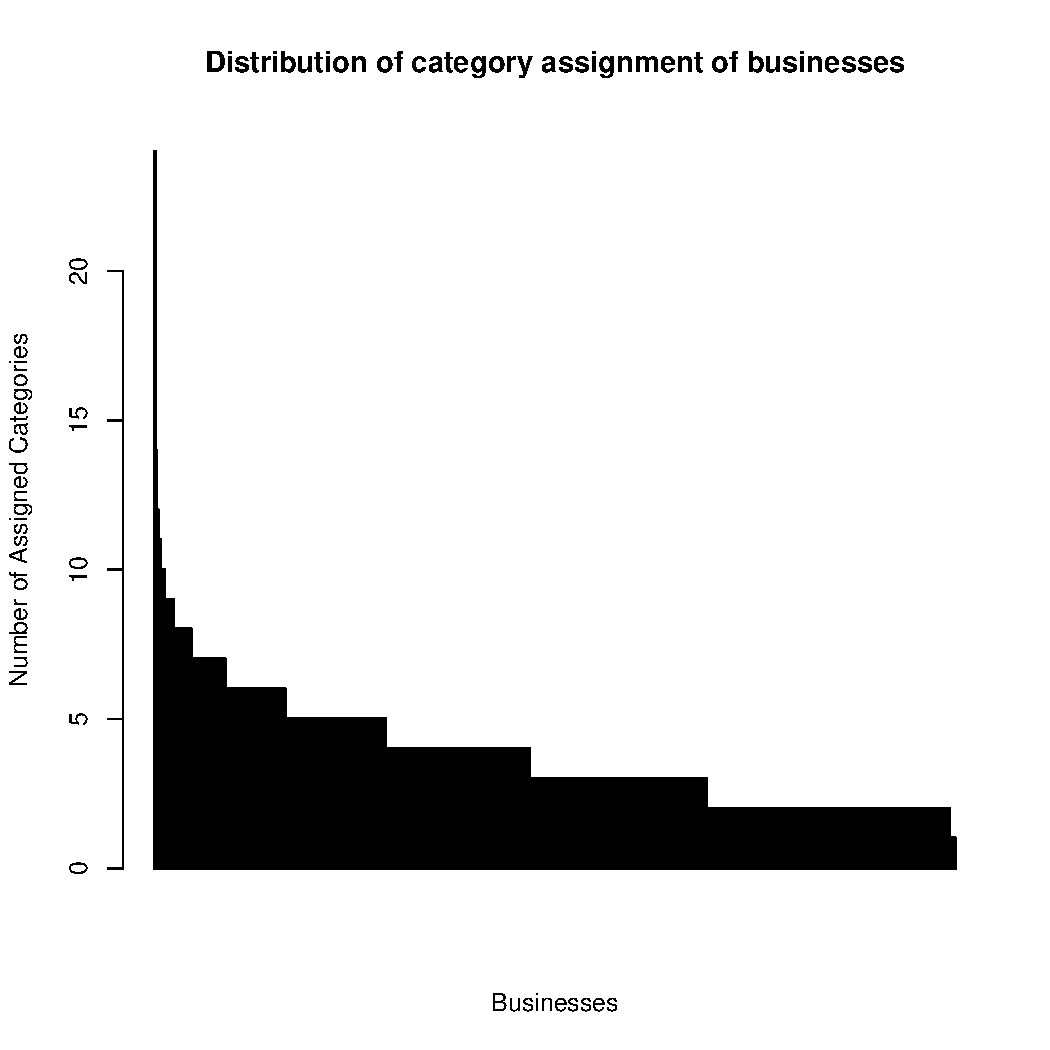
\includegraphics[width=\maxwidth]{figure/unnamed-chunk-29-1} 
\begin{kframe}\begin{alltt}
\hlcom{##sort the frequency of category assignment in descending}
\hlcom{##order and plot the same}
\end{alltt}
\end{kframe}
\end{knitrout}

\begin{DIY}{Think}
\noindent Explain the plot
\end{DIY}

\subsubsection{Joining Data sets}
\noindent \textbf{\underline{Question}}: Which business belong to the category "shopping"?  
\begin{knitrout}
\definecolor{shadecolor}{rgb}{0.969, 0.969, 0.969}\color{fgcolor}\begin{kframe}
\begin{alltt}
\hlstd{shopping} \hlkwb{<-} \hlstd{business[business}\hlopt{$}\hlstd{id} \hlopt
                        \hlstd{businesses_top10Categories}
                            \hlstd{[businesses_top10Categories}\hlopt{$}\hlstd{category}
                                \hlopt{==} \hlstr{"Shopping"}\hlstd{,}
                            \hlstd{]}\hlopt{$}\hlstd{business_id,}
         \hlstd{]}
\hlcom{##list all businesses from the business dataframe }
\hlcom{##that belong to the category "shopping"  }
\hlstd{shopping}
\end{alltt}
\end{kframe}
\end{knitrout}

\begin{DIY}{Think}
\noindent Try using 
\begin{knitrout}
\definecolor{shadecolor}{rgb}{0.969, 0.969, 0.969}\color{fgcolor}\begin{kframe}
\begin{alltt}
\hlstd{businesses_top10Categories[}
          \hlstd{businesses_top10Categories}\hlopt{$}\hlstd{category}
          \hlopt{==} \hlstr{"Shopping"}\hlstd{,}
          \hlstr{"business_id"}
          \hlstd{]}
\end{alltt}
\end{kframe}
\end{knitrout}
instead to get the list of businesses labelled with category = "Shopping". Explain the difference
\end{DIY}


\begin{DIY}{Homework}
\noindent Filter all businesses from the business data frame that belong to one of the top 10 categories
\end{DIY}

\begin{DIY}{Homework}
\noindent Calculate the average reviews count for businesses belonging to the top 10 categories and compare it against the average review count for businesses belonging to the bottom 10 categories
\end{DIY}

\subsection{The \textbf{\emph{attribute}} dataset}
\noindent Import the file \emph{\textbf{attribute.csv}} into your R environment.  


\subsubsection{Dimension and Attributes}
\noindent \textbf{\underline{Question}}: What is the dimension of the data and what are the various attributes?
\begin{knitrout}
\definecolor{shadecolor}{rgb}{0.969, 0.969, 0.969}\color{fgcolor}\begin{kframe}
\begin{alltt}
\hlkwd{dim}\hlstd{(attribute)}
\end{alltt}
\begin{verbatim}
## [1] 1229805       2
\end{verbatim}
\begin{alltt}
\hlcom{##get dimension of the data}
\hlkwd{colnames}\hlstd{(attribute)}
\end{alltt}
\begin{verbatim}
## [1] "business_id" "name"
\end{verbatim}
\begin{alltt}
\hlcom{##get attributes of the data}
\end{alltt}
\end{kframe}
\end{knitrout}

\subsubsection{Filtering, Sorting and Joining }
\noindent \textbf{\underline{Question}}: Which attributes are prevalent for restaurants with 5 star rating?
\begin{knitrout}
\definecolor{shadecolor}{rgb}{0.969, 0.969, 0.969}\color{fgcolor}\begin{kframe}
\begin{alltt}
\hlstd{fiveStarRestaurants}\hlkwb{<-}\hlstd{business[(business}\hlopt{$}\hlstd{id} \hlopt
                  \hlstd{category[}
                            \hlstd{category}\hlopt{$}\hlstd{category} \hlopt{==} \hlstr{"Restaurants"}\hlstd{,}
                         \hlstd{]}\hlopt{$}\hlstd{business_id}
          \hlstd{)}
         \hlopt{&}
         \hlstd{(business}\hlopt{$}\hlstd{stars} \hlopt{==} \hlkwd{max}\hlstd{(business}\hlopt{$}\hlstd{stars)),}
       \hlstd{]}\hlopt{$}\hlstd{id}
\hlcom{##get id's of 5 star restaurants}

\hlstd{attributeCount} \hlkwb{<-} \hlkwd{table}\hlstd{(attribute[}
                                  \hlstd{fiveStarRestaurants}
                                  \hlopt
                                  \hlstd{attribute}\hlopt{$}\hlstd{business_id,}
                                  \hlstr{"name"}\hlstd{]}
                      \hlstd{)}
\hlcom{##find attributes corresponding to the matching business }
\hlcom{##and count their number of occurences }

\hlstd{sortedAttributeCount} \hlkwb{<-} \hlstd{attributeCount[}\hlkwd{order}\hlstd{(}
                                        \hlstd{attributeCount,}
                                        \hlkwc{decreasing} \hlstd{=} \hlnum{TRUE}
                                        \hlstd{)}
                                      \hlstd{]}
\hlcom{##sort the attributes in descending order of their occurence}

\hlstd{sortedAttributePercent} \hlkwb{<-} \hlstd{sortedAttributeCount} \hlopt{/} \hlkwd{sum}\hlstd{(sortedAttributeCount)} \hlopt{*} \hlnum{100}
\hlcom{##normalize the counts                              }

\hlkwd{par}\hlstd{(}\hlkwc{las}\hlstd{=}\hlnum{2}\hlstd{)}
\hlcom{##make lable text perpendicular to the axis}

\hlkwd{par}\hlstd{(}\hlkwc{mar}\hlstd{=}\hlkwd{c}\hlstd{(}\hlnum{5}\hlstd{,}\hlnum{12}\hlstd{,}\hlnum{4}\hlstd{,}\hlnum{2}\hlstd{))}
\hlcom{##increase y-axis margin}

\hlkwd{barplot}\hlstd{(sortedAttributePercent[sortedAttributePercent} \hlopt{>} \hlnum{1}\hlstd{],}
        \hlkwc{horiz}\hlstd{=}\hlnum{TRUE}\hlstd{,}
        \hlkwc{cex.names} \hlstd{=} \hlnum{0.8}\hlstd{,}
        \hlkwc{xlab} \hlstd{=} \hlstr{"% of occurence"}\hlstd{,}
        \hlkwc{main} \hlstd{=} \hlstr{"Distribution of attributes for 5 star restaurants"}\hlstd{)}
\end{alltt}
\end{kframe}
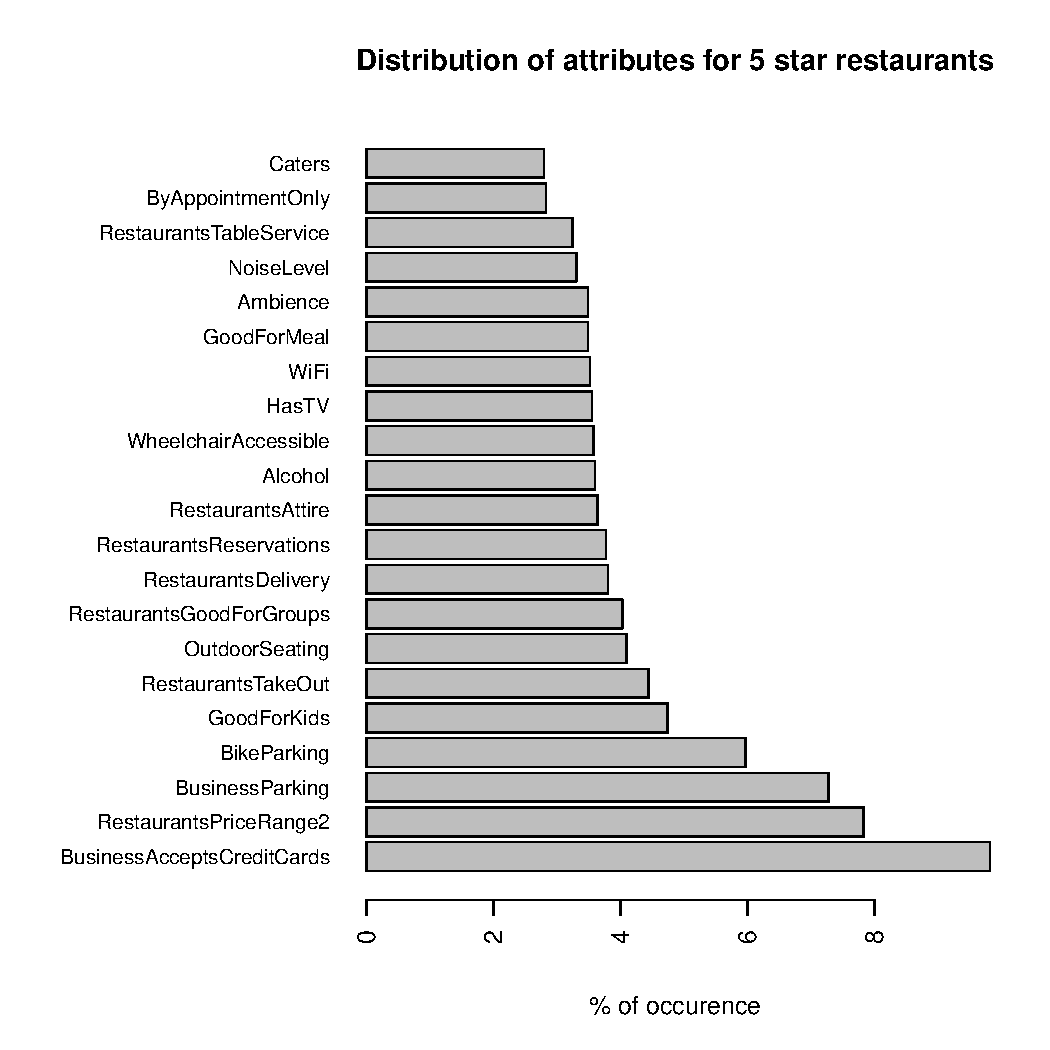
\includegraphics[width=\maxwidth]{figure/prevalentAttributes-1} 
\begin{kframe}\begin{alltt}
\hlcom{##plot the distribution of attributes }
\hlcom{##that occur at least 1% of the time}
\end{alltt}
\end{kframe}
\end{knitrout}

\begin{DIY}{Warning}
\noindent Pay close attention to the \textbf{\emph{par()}} function in the example
\end{DIY}

\begin{DIY}{Homework}
\noindent Read the help manual of the \textbf{\emph{par()}} function
\end{DIY}

\begin{DIY}{Homework}
\noindent\begin{itemize}
  \item Which attributes are prevalent for restaurants with 3 star rating? Compare the same with attributes of restaurants that have a rating of 5 stars. Explain your observation
  \item Do the same analysis for businesses which have category as "Shopping" 
\end{itemize}
\end{DIY}


%\subsection{dplyr}
%\subsection{data.table}

%<<DataVisualization,child='./DataVisualization.Rnw'>>=
%@


% !Rnw root = Introduction.Rnw
\newpage
%===============================
\section{Control Structures}
%===============================

\subsection{The \textbf{\emph{checkin}} dataset}
\noindent Import the file \emph{\textbf{checkin.csv}} into your R environment. 


\subsubsection{Dimension and Attributes}
\noindent \textbf{\underline{Question}}: What is the dimension of the data and what are the various attributes?
\begin{knitrout}
\definecolor{shadecolor}{rgb}{0.969, 0.969, 0.969}\color{fgcolor}\begin{kframe}
\begin{alltt}
\hlkwd{dim}\hlstd{(checkin)}
\end{alltt}
\begin{verbatim}
## [1] 3738750       3
\end{verbatim}
\begin{alltt}
\hlcom{##get dimension of the data}
\hlkwd{colnames}\hlstd{(checkin)}
\end{alltt}
\begin{verbatim}
## [1] "business_id" "date"        "count"
\end{verbatim}
\begin{alltt}
\hlcom{##get attributes of the data}
\end{alltt}
\end{kframe}
\end{knitrout}

\subsubsection{Splitting Strings}
\noindent \textbf{\underline{Question}}: How can we split the checkin date (DayOfWeek-HH:MM) into "day of week" and "time"?
\begin{knitrout}
\definecolor{shadecolor}{rgb}{0.969, 0.969, 0.969}\color{fgcolor}\begin{kframe}
\begin{alltt}
\hlstd{checkinTime} \hlkwb{<-} \hlkwd{strsplit}\hlstd{(checkin}\hlopt{$}\hlstd{date,}\hlkwc{split} \hlstd{=} \hlstr{"-"}\hlstd{)}
\hlcom{## split the date string into day of week and time}
\end{alltt}
\end{kframe}
\end{knitrout}

\begin{DIY}{Homework}
\noindent Read the help manual of the \textbf{\emph{strsplit()}} function
\end{DIY}

\begin{DIY}{Think}
\noindent What is the type of the object "checkinTime"? 
\end{DIY}

\newpage
\subsection{The \textbf{\emph{for}} loop}
\begin{HIGHLIGHT}
\par\noindent{
{\centering\textbf{\emph{for(name in range) body}} \\}
}
\end{HIGHLIGHT}

\subsubsection{Iterative Vectorization}
\noindent \textbf{\underline{Question}}: How can we create three vectors for "day of week", "hour of day" and "minutes" respectively?
\begin{knitrout}
\definecolor{shadecolor}{rgb}{0.969, 0.969, 0.969}\color{fgcolor}\begin{kframe}
\begin{alltt}
\hlstd{numCheckins} \hlkwb{<-} \hlkwd{length}\hlstd{(checkinTime)}
\hlcom{##the length of the list that contains }
\hlcom{## lists of the form [[<day of week>,<hour of day>,<minute>],..] }
\hlstd{dow} \hlkwb{<-} \hlkwd{vector}\hlstd{(}\hlkwc{mode} \hlstd{=} \hlstr{"character"}\hlstd{,} \hlkwc{length} \hlstd{= numCheckins)}
\hlcom{## a character vector of size = numCheckins}
\hlstd{hod} \hlkwb{<-} \hlkwd{vector}\hlstd{(}\hlkwc{mode} \hlstd{=} \hlstr{"integer"}\hlstd{,} \hlkwc{length} \hlstd{= numCheckins)}
\hlcom{## an integer vector of size = numCheckins}
\hlstd{minute} \hlkwb{<-} \hlkwd{vector}\hlstd{(}\hlkwc{mode} \hlstd{=} \hlstr{"integer"}\hlstd{,} \hlkwc{length} \hlstd{= numCheckins)}
\hlcom{## an integer vector of size = numCheckins}
\hlstd{index} \hlkwb{=} \hlnum{1} \hlcom{##set increment counter to 1}
\hlkwa{for} \hlstd{(dayTime} \hlkwa{in} \hlstd{checkinTime)\{}
      \hlcom{## iterateve over each list in the list}
      \hlstd{dow[index]}\hlkwb{<-}\hlstd{dayTime[}\hlnum{1}\hlstd{]}
      \hlcom{## extract the first element of the list (day of week)}
      \hlcom{## and assign it to the corresponding position in dow}
      \hlstd{HH_MM_split} \hlkwb{<-} \hlkwd{strsplit}\hlstd{(dayTime[}\hlnum{2}\hlstd{],}\hlkwc{split} \hlstd{=} \hlstr{":"}\hlstd{)}
      \hlcom{## split the second element }
      \hlcom{## of the list (HH:MM) into HH and MM which in turn }
      \hlcom{##creates a list of lists}
      \hlstd{hod[index]} \hlkwb{<-} \hlkwd{as.integer}\hlstd{(HH_MM_split[[}\hlnum{1}\hlstd{]][}\hlnum{1}\hlstd{])}
      \hlcom{##access the first element (hour)}
      \hlcom{## of the list of lists  and assign it to the }
      \hlcom{##corresponding position in hod}
      \hlstd{minute[index]} \hlkwb{<-} \hlkwd{as.integer}\hlstd{(HH_MM_split[[}\hlnum{1}\hlstd{]][}\hlnum{2}\hlstd{])}
      \hlcom{##access the second element (minute)}
      \hlcom{## of the list of lists and assign it to the }
      \hlcom{##corresponding position in minute}
      \hlstd{index} \hlkwb{=} \hlstd{index} \hlopt{+} \hlnum{1} \hlcom{##increment the value of index}
\hlstd{\}}
\hlstd{index} \hlkwb{=} \hlnum{1} \hlcom{##reset index to 1}
\end{alltt}
\end{kframe}
\end{knitrout}

\begin{DIY}{Think}
\begin{itemize}
  \item \noindent Explain the meaning of the \textbf{[[]]} in the context of the example
  \item \noindent What happens if we set the mode of the vectors "hod" and "minute" to \textbf{\emph{numeric}}?
\end{itemize}
\end{DIY}

\begin{DIY}{Homework}
 \begin{itemize}
  \item \noindent Install the package \textbf{rbenchmark} and read the help manual for the \textbf{\emph{benchmark()}} function.
  \item \noindent Try the above example without initializing the length/type of the vector. Benchmark the same against the given example. Explain why do you see a difference in the execution time
  \item \noindent Do not reset the index value to 1 at the end of the example and run the code block twice. Observe the size of the vectors "dow", "hod" and "minute". Explain your observation.  
\end{itemize}
\end{DIY}

\subsection{The \textbf{\emph{if}} statement}
\label{sec: conditionalStatements}
\begin{HIGHLIGHT}
\par\noindent{
{\centering\textbf{\emph{if(test) expression1 else expression2}} \\}
}
\end{HIGHLIGHT}

\subsubsection{Conditional Assignment}
\noindent \textbf{\underline{Question}}: How can we map days of week to their position in the week? e.g. Sunday = 0, Monday = 1, $....$
\begin{knitrout}
\definecolor{shadecolor}{rgb}{0.969, 0.969, 0.969}\color{fgcolor}\begin{kframe}
\begin{alltt}
\hlstd{pow} \hlkwb{<-} \hlkwd{vector}\hlstd{(}\hlkwc{mode} \hlstd{=} \hlstr{"integer"}\hlstd{,} \hlkwc{length} \hlstd{=} \hlkwd{length}\hlstd{(dow))}
\hlcom{## create a vector of type integer where the length is }
\hlcom{## equal to the number of elements in the dow}
\hlstd{index} \hlkwb{=} \hlnum{1} \hlcom{## set the increment counter to 1}
\hlkwa{for}\hlstd{(item} \hlkwa{in} \hlstd{dow)\{} \hlcom{##iterate over element of the the }
  \hlcom{## day of week vector}
       \hlkwa{if} \hlstd{(item} \hlopt{==} \hlstr{"Sunday"}\hlstd{)\{}
         \hlstd{pow[index]} \hlkwb{<-} \hlnum{0} \hlcom{## if the day of week is sunday assign}
         \hlcom{## value 0 to the corresponding position in the pow vector}
      \hlstd{\}}
      \hlkwa{if} \hlstd{(item} \hlopt{==} \hlstr{"Monday"}\hlstd{)\{}
         \hlstd{pow[index]} \hlkwb{<-} \hlnum{1} \hlcom{## if the day of week is monday assign}
         \hlcom{## value 1 to the corresponding position in the pow vector}
      \hlstd{\}}
      \hlkwa{else if} \hlstd{(item} \hlopt{==} \hlstr{"Tuesday"}\hlstd{)\{}
         \hlstd{pow[index]} \hlkwb{<-} \hlnum{2} \hlcom{## if the day of week is tuesday assign}
         \hlcom{## value 2 to the corresponding position in the pow vector}
      \hlstd{\}}
      \hlkwa{else if} \hlstd{(item} \hlopt{==} \hlstr{"Wednesday"}\hlstd{)\{}
         \hlstd{pow[index]} \hlkwb{<-} \hlnum{3} \hlcom{## if the day of week is wednesday assign}
         \hlcom{## value 3 to the corresponding position in the pow vector}
      \hlstd{\}}
      \hlkwa{else if} \hlstd{(item} \hlopt{==} \hlstr{"Thursday"}\hlstd{)\{}
         \hlstd{pow[index]} \hlkwb{<-} \hlnum{4} \hlcom{## if the day of week is thursday assign}
         \hlcom{## value 4 to the corresponding position in the pow vector}
      \hlstd{\}}
     \hlkwa{else if} \hlstd{(item} \hlopt{==} \hlstr{"Friday"}\hlstd{)\{}
         \hlstd{pow[index]} \hlkwb{<-} \hlnum{5} \hlcom{## if the day of week is friday assign}
         \hlcom{## value 5 to the corresponding position in the pow vector}
     \hlstd{\}}
     \hlkwa{else if} \hlstd{(item} \hlopt{==} \hlstr{"Saturday"}\hlstd{)\{}
         \hlstd{pow[index]} \hlkwb{<-} \hlnum{6} \hlcom{## if the day of week is saturday assign}
         \hlcom{## value 6 to the corresponding position in the pow vector}
     \hlstd{\}}
     \hlstd{index} \hlkwb{=} \hlstd{index} \hlopt{+} \hlnum{1} \hlcom{##increment the value of index}
\hlstd{\}}
\hlstd{index} \hlkwb{=} \hlnum{1}  \hlcom{##reset index to 1}
\end{alltt}
\end{kframe}
\end{knitrout}





\begin{DIY}{Homework}
 \begin{itemize}
  \item \noindent How can you achieve the same result without using the \emph{for loop} and \emph{if statement} at all! \textcolor{red}{Hint:} try the \textbf{\emph{which()}} function. Benchmark your implementation (without the control statements) against the example. Do you notice a difference in performance? Explain your observation.
  \item \noindent Create a data frame named \emph{checkins} that has the following attributes
\end{itemize}
\end{DIY}

\begin{knitrout}
\definecolor{shadecolor}{rgb}{0.969, 0.969, 0.969}\color{fgcolor}\begin{kframe}
\begin{alltt}
 \hlkwd{colnames}\hlstd{(checkins)}
\end{alltt}
\begin{verbatim}
## [1] "business_id"      "day_of_week"      "position_of_week"
## [4] "hour"             "minute"           "count"
\end{verbatim}
\end{kframe}
\end{knitrout}

\subsubsection{Validation}
\noindent \textbf{\underline{Question}}: How can we check for correct assignment of position to day of week?
\begin{knitrout}
\definecolor{shadecolor}{rgb}{0.969, 0.969, 0.969}\color{fgcolor}\begin{kframe}
\begin{alltt}
\hlkwd{table}\hlstd{(checkins}\hlopt{$}\hlstd{day_of_week,checkins}\hlopt{$}\hlstd{position_of_week)}
\end{alltt}
\begin{verbatim}
##            
##                  0      1      2      3      4      5      6
##   Friday         0      0      0      0      0 558419      0
##   Monday         0 478652      0      0      0      0      0
##   Saturday       0      0      0      0      0      0 624409
##   Sunday    542932      0      0      0      0      0      0
##   Thursday       0      0      0      0 520651      0      0
##   Tuesday        0      0 499441      0      0      0      0
##   Wednesday      0      0      0 514246      0      0      0
\end{verbatim}
\begin{alltt}
\hlcom{##co-occurence count of day of week and position}
\hlkwd{sum}\hlstd{(}\hlkwd{table}\hlstd{(checkins}\hlopt{$}\hlstd{day_of_week,checkins}\hlopt{$}\hlstd{position_of_week))} \hlopt{==}
  \hlkwd{dim}\hlstd{(checkins)[}\hlnum{1}\hlstd{]}
\end{alltt}
\begin{verbatim}
## [1] TRUE
\end{verbatim}
\begin{alltt}
\hlcom{##check if every day of week has been mapped to one position}
\end{alltt}
\end{kframe}
\end{knitrout}

\begin{DIY}{Think}
\noindent Explain the output of the code snippet 
\end{DIY}

\begin{DIY}{Homework}
\noindent Compute the total number of checkins aggregated by hour and day of week. Plot the same 
\end{DIY}

\newpage
\subsubsection{Conditional Distribution}
\noindent \textbf{\underline{Question}}: What is the distribution of checkins over each day of the week?
\begin{knitrout}
\definecolor{shadecolor}{rgb}{0.969, 0.969, 0.969}\color{fgcolor}\begin{kframe}
\begin{alltt}
\hlkwd{summary}\hlstd{(checkins}\hlopt{$}\hlstd{count)}
\end{alltt}
\begin{verbatim}
##    Min. 1st Qu.  Median    Mean 3rd Qu.    Max. 
##       1       1       2       4       3    1420
\end{verbatim}
\begin{alltt}
\hlcom{##generate summary statistic for checkin count}
\hlkwd{boxplot}\hlstd{(checkins}\hlopt{$}\hlstd{count} \hlopt{~} \hlstd{checkins}\hlopt{$}\hlstd{day_of_week,}
        \hlkwc{main} \hlstd{=} \hlstr{"Distribution of checkins over days of week"}\hlstd{,}
        \hlkwc{xlab} \hlstd{=} \hlstr{"day of week"}\hlstd{,}\hlkwc{ylab} \hlstd{=} \hlstr{"Number of checkins"}\hlstd{)}
\end{alltt}
\end{kframe}
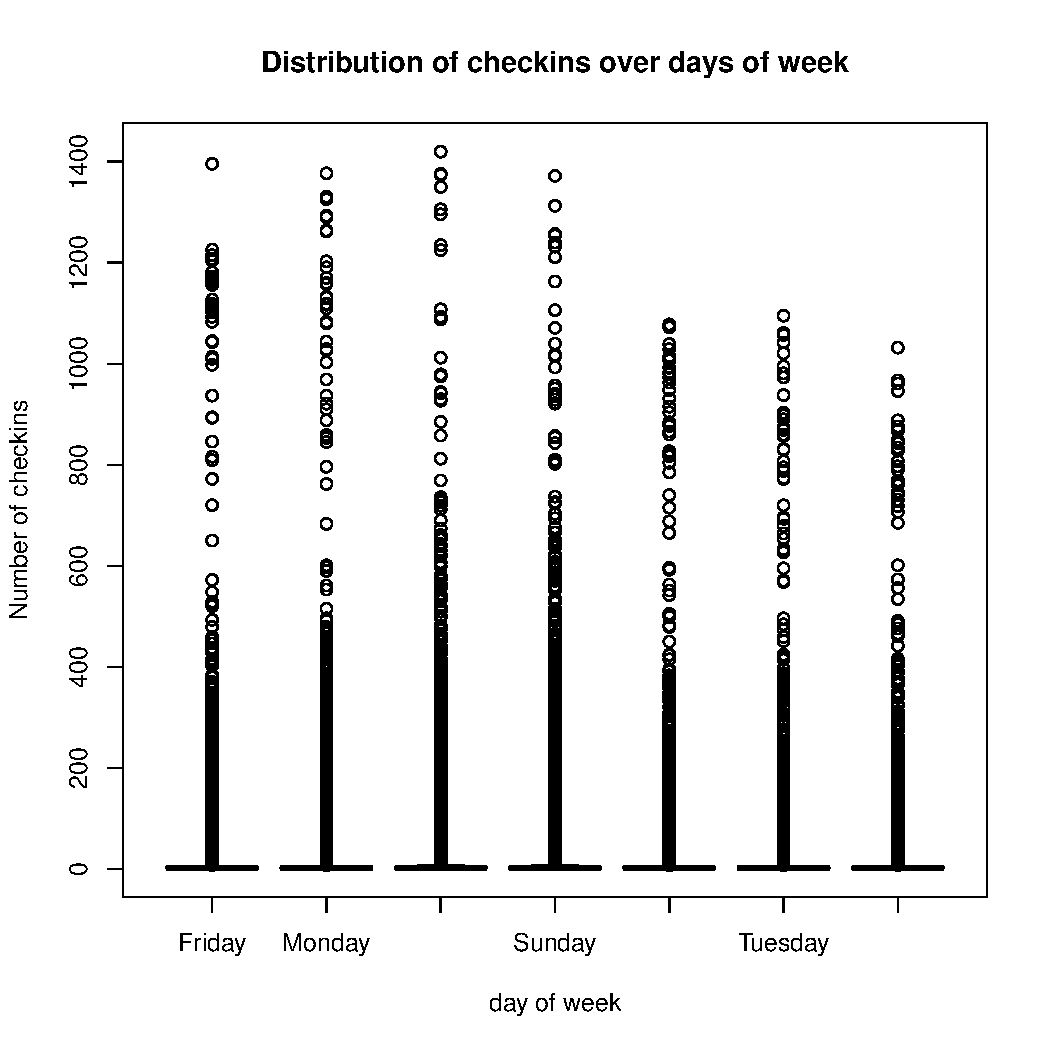
\includegraphics[width=\maxwidth]{figure/checkinsOverWeek-1} 
\begin{kframe}\begin{alltt}
\hlcom{##distribution of count , given, day of week}
\end{alltt}
\end{kframe}
\end{knitrout}

\begin{DIY}{Think}
\noindent Explain the plot
\end{DIY}

\begin{DIY}{Homework}
\begin{itemize}
  \item \noindent Regenerate the plot but only for checkins $\geq$ 3rd Quartile
  \item \noindent Generate a plot that shows the relationship between hour of day and number of checkins. Explain if you notice a relationship between the two
\end{itemize}
\end{DIY}


% !Rnw root = Introduction.Rnw
\newpage
%===============================
\section{Functions}
\label{sec:functions}
%===============================
\begin{HIGHLIGHT}
\par\noindent{
{\centering\textbf{function(arguments) body} \\}
}
\end{HIGHLIGHT}
\noindent \textbf{\underline{Question}}: How can we split the "date" attribute into "day of week", "hour of day" and "minutes" respectively?
\begin{knitrout}
\definecolor{shadecolor}{rgb}{0.969, 0.969, 0.969}\color{fgcolor}\begin{kframe}
\begin{alltt}
\hlcom{## a generic splitting function that accepts as arguments}
\hlcom{## - an input of type characer that is to be split }
\hlcom{## - the delimiter for day}
\hlcom{## - the delimiter for time}
\hlcom{## returns : a list of the form }
\hlcom{##           [<day of week>, <hour of day>, <minute>]}
\hlstd{getDOW_HOD} \hlkwb{<-} \hlkwa{function}\hlstd{(}\hlkwc{dateString}\hlstd{,}\hlkwc{dowSplitter} \hlstd{=} \hlstr{""}\hlstd{,}\hlkwc{timeSplitter} \hlstd{=} \hlstr{""}\hlstd{)\{}
            \hlstd{splitValues} \hlkwb{<-} \hlkwd{strsplit}\hlstd{(dateString,}\hlkwc{split} \hlstd{= dowSplitter)}
            \hlstd{dow} \hlkwb{<-} \hlstd{splitValues[[}\hlnum{1}\hlstd{]][}\hlnum{1}\hlstd{]}
            \hlstd{HH_MM_split} \hlkwb{<-} \hlkwd{strsplit}\hlstd{(splitValues[[}\hlnum{1}\hlstd{]][}\hlnum{2}\hlstd{],}
                                    \hlkwc{split} \hlstd{= timeSplitter)}
            \hlstd{hod} \hlkwb{<-} \hlkwd{as.numeric}\hlstd{(HH_MM_split[[}\hlnum{1}\hlstd{]][}\hlnum{1}\hlstd{])}
            \hlstd{mod} \hlkwb{<-} \hlkwd{as.numeric}\hlstd{(HH_MM_split[[}\hlnum{1}\hlstd{]][}\hlnum{2}\hlstd{])}
            \hlkwd{return}\hlstd{(}\hlkwd{list}\hlstd{(}\hlkwc{dayOfWeek} \hlstd{= dow,}
                        \hlkwc{hourOfDay} \hlstd{= hod,}
                        \hlkwc{minute} \hlstd{= mod))}
\hlstd{\}}

\hlcom{## for every elment in checkin\textbackslash{}$date apply the }
\hlcom{## function getDOW_HOD}
\hlstd{result} \hlkwb{<-} \hlkwd{lapply}\hlstd{(checkin}\hlopt{$}\hlstd{date,}
                 \hlstd{getDOW_HOD,}
                 \hlkwc{dowSplitter} \hlstd{=} \hlstr{'-'}\hlstd{,}\hlkwc{timeSplitter} \hlstd{=} \hlstr{':'}
                \hlstd{)}
\end{alltt}
\end{kframe}
\end{knitrout}

\begin{DIY}{Think}
\noindent Read the help manual for \textbf{\emph{lapply()}}. Try using \textbf{\emph{apply()}} instead of \textbf{\emph{lapply()}}.
\end{DIY}

\begin{DIY}{Warning}
\textcolor{red}{The reader is urged to work on the following exercise!}
\end{DIY}

\begin{DIY}{Homework}
\noindent \textcolor{red}{Write a R function that:} Given a category and time of week e.g (weekday/weekend),(morning/evening), the function should compute the number of checkins per state. Moreover, the function should also check if there exists a relationship between the rating of a business and the number of checkins 
The function should also generate plots that visualize the results.
\end{DIY}



\newpage
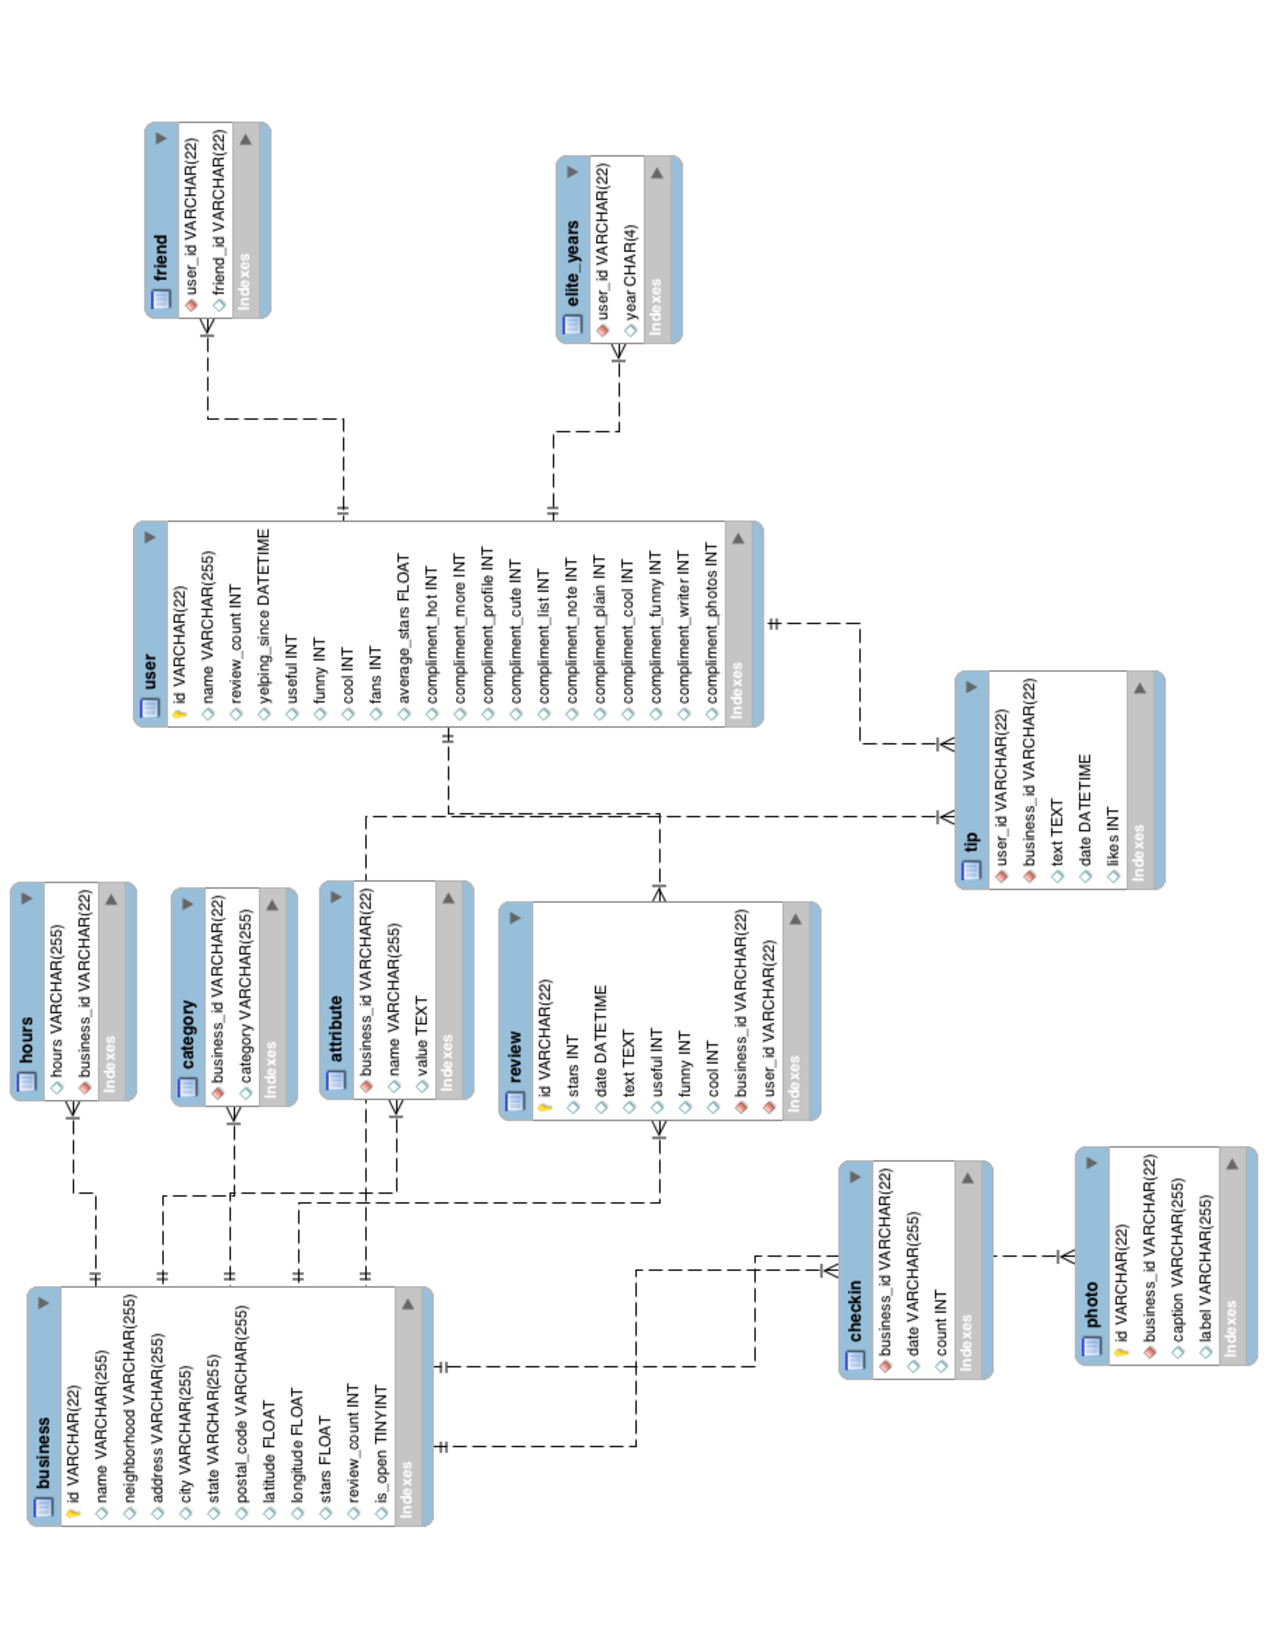
\includepdf[pages={1}]{./References/yelp_dataset_schema.pdf}

\cleardoublepage
\thispagestyle{empty}
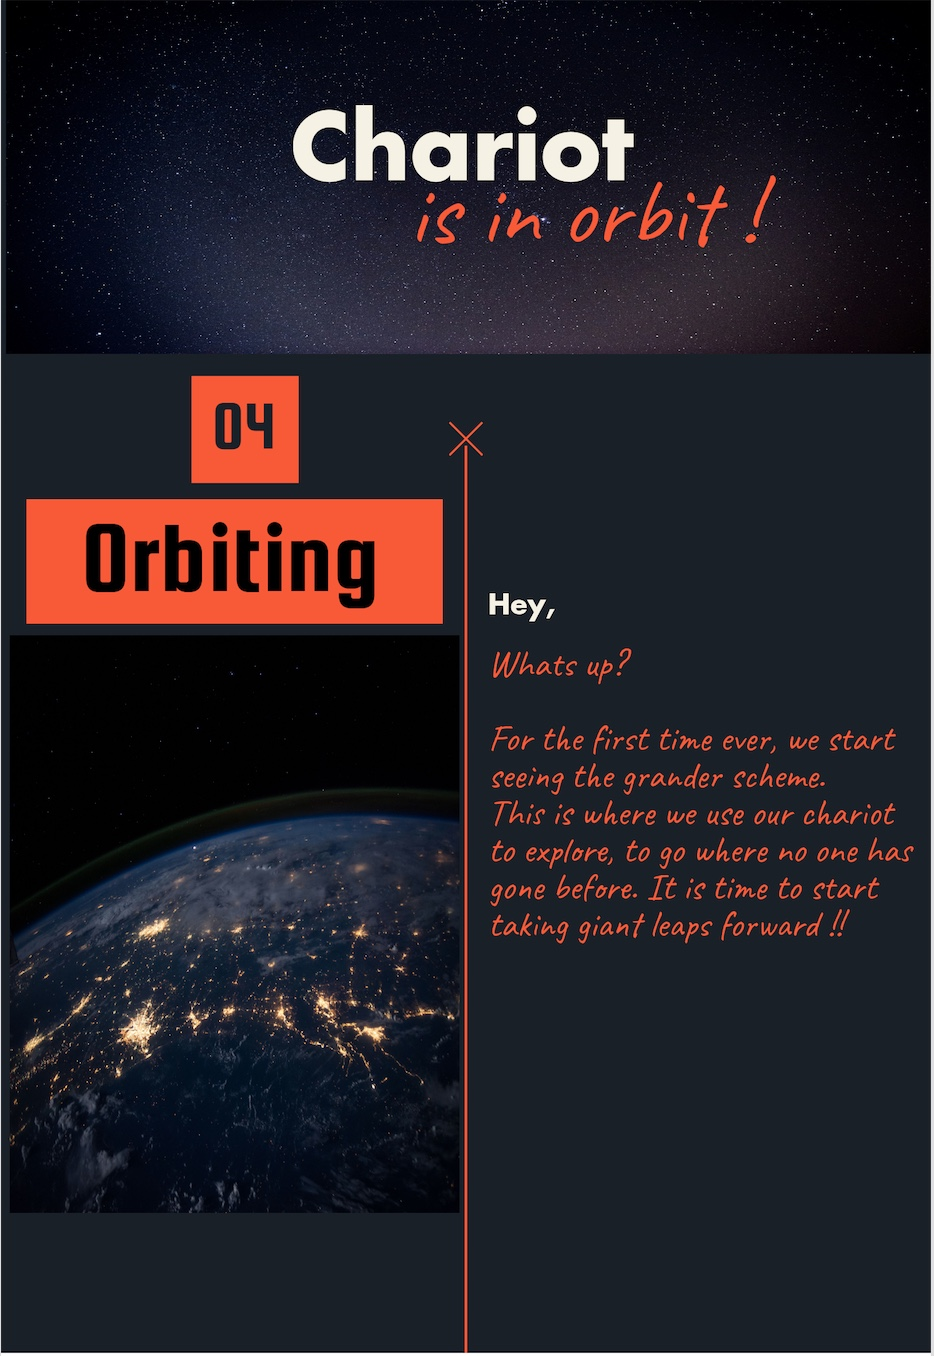
\includegraphics[width = 16 cm]{./viz/ext/Orbit.jpeg}
%=======================================
 \chapter{The Orbiting}
%=======================================

% !Rnw root = main.Rnw
%===============================
\section{The Grammar of Graphics}
%===============================

\begin{HIGHLIGHT}
\par\noindent{
\noindent \textbf{\emph{The Grammar of Graphics}} provides a formal, structured perspective on how to describe data graphics. Therefore, the grammar of graphics is a \emph{mapping from 
properties of data to visual properties of graphics}. The data properties are typically numerical or categorical values, while the visual properties include the \emph{x} and \emph{y} position of points, colors of lines, heights of bars and so on.
}
\end{HIGHLIGHT}

\noindent Over the past years, \textbf{\emph{ggplot2}} has become the de-facto package for data visualization in R. In this chapter, we will familiarize the reader with the basic concepts of ggplot2 and show basic data visualization techniques using the same. For a more detailed and thorough treatment please refer to the following book. Moreover, a large number of examples using ggplot2 can be found at \textcolor{cyan}{\url{http://r-statistics.co/Complete-Ggplot2-Tutorial-Part1-With-R-Code.html}}. Furthermore, a cheatsheet for ggplot2() is available in the RStudio IDE and can be found at the end of this chapter as well.    

\begin{figure}[ht]
      \centering
      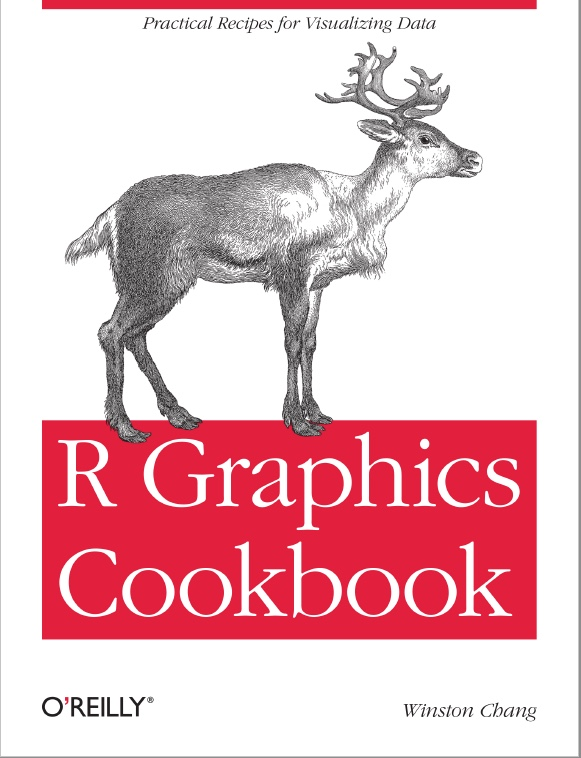
\includegraphics[width = 6 cm]{./viz/ext/RCookbook.jpeg}
\end{figure}


% !Rnw root = main.Rnw
%===============================
\section{The ggplot2 Package}
%===============================

\begin{DIY}{Warning}
\noindent \textcolor{red}{ggplot2 is not bundled with the base packages of R. So the user will have to install ggplot2 before being able to use it.}
\end{DIY}

\begin{HIGHLIGHT}
\par\noindent{
{\centering\textbf{\emph{\Large ggplot2 Terminology}} \\}
\vspace{\baselineskip}
\begin{enumerate}
      \item \textbf{\emph{Data}} is what we want to visualize. It consists of \emph{variables} which are stored as columns in
      a data frame.
      \item \textbf{\emph{Geoms}} are the geometric objects that are drawn to represent the data, such as bars, lines, and points.
      \item \textbf{\emph{Aesthetics}} are visual properties of geoms, such as x and y position, line color, point shapes, etc.
      \item \textbf{\emph{Mappings}} represent the relationship between data values and aesthetics.
      \item \textbf{\emph{Scales}} control the mapping from the the values in the data space, to values in the aesthetics space. 
      \item \textbf{\emph{Guides}} show the viewer how to map the visual properties back to the data space. Commonly used guides are tick marks and labels on an axis.
\end{enumerate}
}
\end{HIGHLIGHT}

\begin{DIY}{Warning}
\noindent \textcolor{red}{ggplot2 requires the data to be represented as a data frame wherein each variable, that is mapped to an asthetic must be represented as a column in the data frame.
}
\end{DIY}

\begin{DIY}{Warning}
\noindent ggplot2 uses the '$+$' operator to add, each of the components described above, to a visualization. Recall that the '$+$' operator is a function in R and the operands (in this case ggplot2 functions) are arguments to this function.
\end{DIY}

\begin{DIY}{Warning}
\noindent The reader is urged to pay close attention to the comments section of the code snippets in this chapter, as the workings of ggplot2 has been explained in those comments.
\end{DIY}



\newpage
\subsection{A Step By Step Guide To Visualization with ggplot2}
\noindent \textbf{\Large \underline{Step 1}}: {\Large Add the \emph{data frame} that you wish to visualize}
\begin{knitrout}
\definecolor{shadecolor}{rgb}{0.969, 0.969, 0.969}\color{fgcolor}\begin{kframe}
\begin{alltt}
\hlstd{graph} \hlkwb{<-} \hlkwd{ggplot}\hlstd{(business)}
\hlcom{##pass data frame to ggplot2}
\hlstd{graph}
\end{alltt}
\end{kframe}

\includegraphics[width=\maxwidth]{figure/add_data_frame-1} 

\end{knitrout}

\begin{DIY}{Warning}
\noindent Passing a data frame to the ggplot() function initializes a ggplot visualization without any axis or points i.e without any aesthetics. The next step is to add aesthetics to the plot.
\end{DIY}

\newpage
\noindent \textbf{\Large \underline{Step 2}}: {\Large Set the \emph{Aesthetics} of the visualization} 
\begin{knitrout}
\definecolor{shadecolor}{rgb}{0.969, 0.969, 0.969}\color{fgcolor}\begin{kframe}
\begin{alltt}
\hlstd{graph} \hlkwb{<-} \hlstd{graph} \hlopt{+}
\hlkwd{aes}\hlstd{(} \hlkwc{x} \hlstd{= business}\hlopt{$}\hlstd{review_count,}
     \hlkwc{y} \hlstd{= business}\hlopt{$}\hlstd{stars}
\hlstd{)}
\hlcom{##set the aesthetics of the x and y axis by mapping }
\hlcom{## review count to the x axis and stars to the y axis}
\hlstd{graph}
\end{alltt}
\end{kframe}
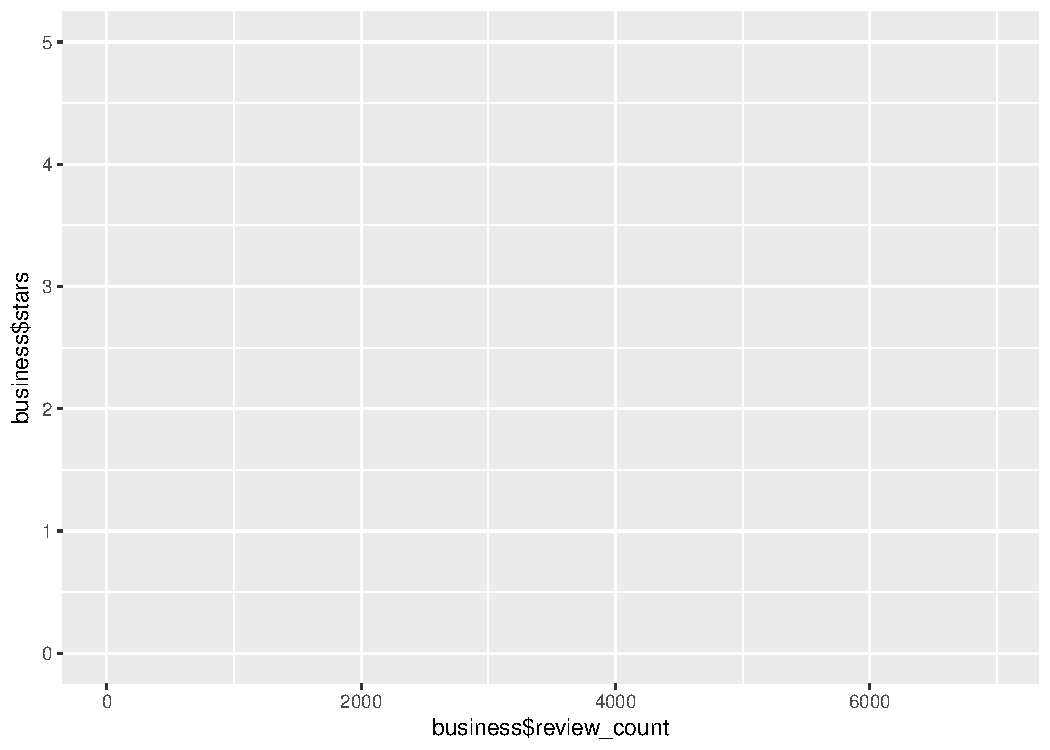
\includegraphics[width=\maxwidth]{figure/add_aesthetics-1} 

\end{knitrout}

\begin{DIY}{Warning}
\noindent Adding aesthetics to the plot results in addition of coordinate axis to the plot. As in the case of base graphics in R, one may need to create both or at least one axis using aesthetics. Note, that the argument passed to the \emph{aes()} function defines a \emph{mapping} from the columns in the data frame to its corresponding visual representation. Moreover, the axis labels are set to the column names by default. We will change this in the next steps.
\end{DIY}

\newpage
\noindent \textbf{\Large \underline{Step 3}}: {\Large Add \emph{Geometry} to the visualization} 
\begin{knitrout}
\definecolor{shadecolor}{rgb}{0.969, 0.969, 0.969}\color{fgcolor}\begin{kframe}
\begin{alltt}
\hlstd{graph} \hlkwb{<-} \hlstd{graph} \hlopt{+} \hlkwd{geom_point}\hlstd{()}
\hlcom{## add geometry and more specifically tell ggplot}
\hlcom{## to add points for (x,y) values}
\hlstd{graph}
\end{alltt}
\end{kframe}
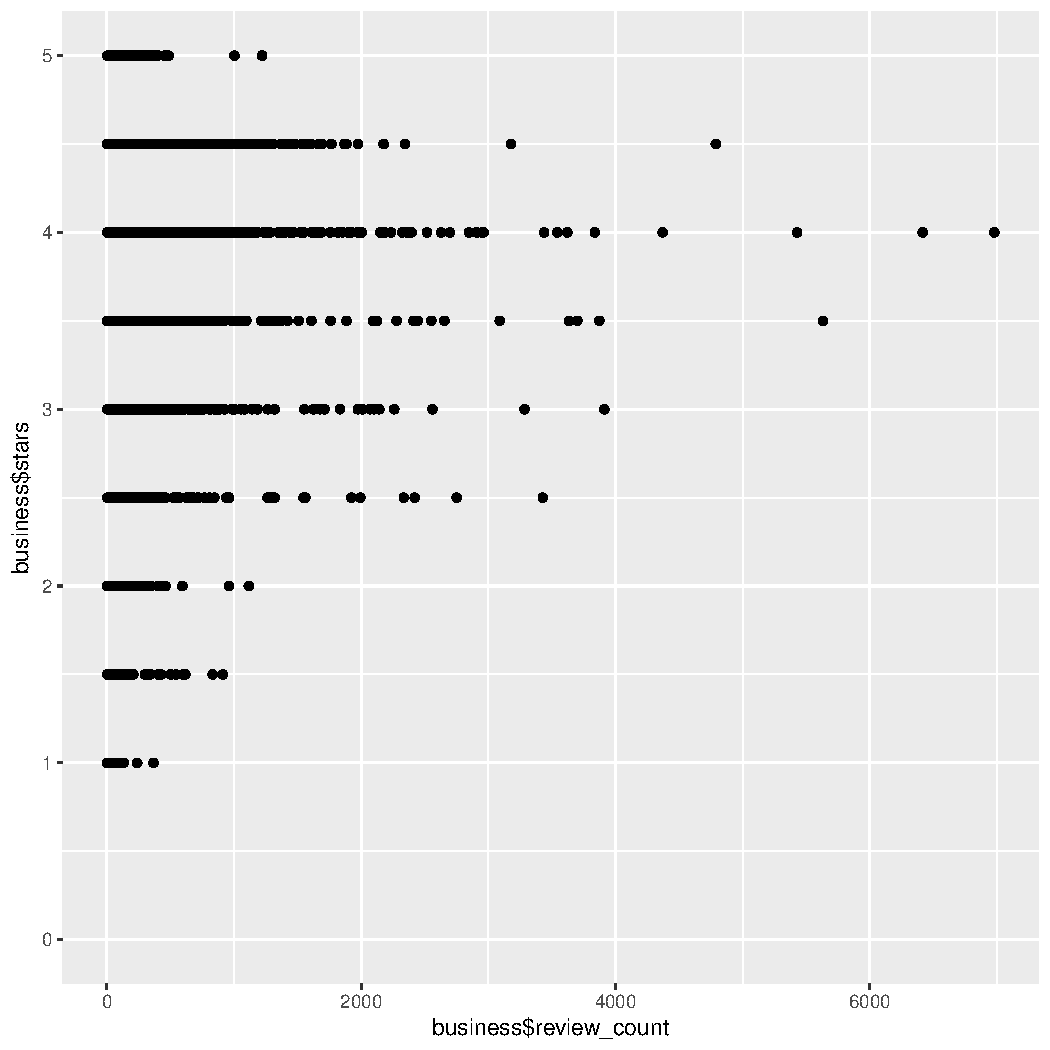
\includegraphics[width=\maxwidth]{figure/add_geometry-1} 

\end{knitrout}

\begin{DIY}{Warning}
\noindent Adding geometry, instructs the visualization system to generate a particular type of plot. For example \emph{geom\textunderscore point()} would generate a scatter plot, \emph{geom\textunderscore bar()} would generate a bar plot,
 \emph{geom\textunderscore hist()} would generate a histogram etc.
\end{DIY}

\newpage
\noindent \textbf{\Large \underline{Step 4}}: {\Large Add \emph{Guides} to the visualization} 
\begin{knitrout}
\definecolor{shadecolor}{rgb}{0.969, 0.969, 0.969}\color{fgcolor}\begin{kframe}
\begin{alltt}
\hlstd{graph} \hlkwb{<-} \hlstd{graph} \hlopt{+}
\hlkwd{ggtitle}\hlstd{(} \hlstr{"Relationship between Reviews wrt Ratings"}\hlstd{,}
           \hlkwc{subtitle} \hlstd{=} \hlstr{"A Scatterplot"} \hlstd{)} \hlopt{+}
\hlkwd{xlab}\hlstd{(}\hlstr{"Reviews"}\hlstd{)} \hlopt{+} \hlkwd{ylab}\hlstd{(}\hlstr{"Ratings"}\hlstd{)}
\hlcom{## add title and subtitle to the plot}
\hlcom{## add labels to the axis}
\hlstd{graph}
\end{alltt}
\end{kframe}
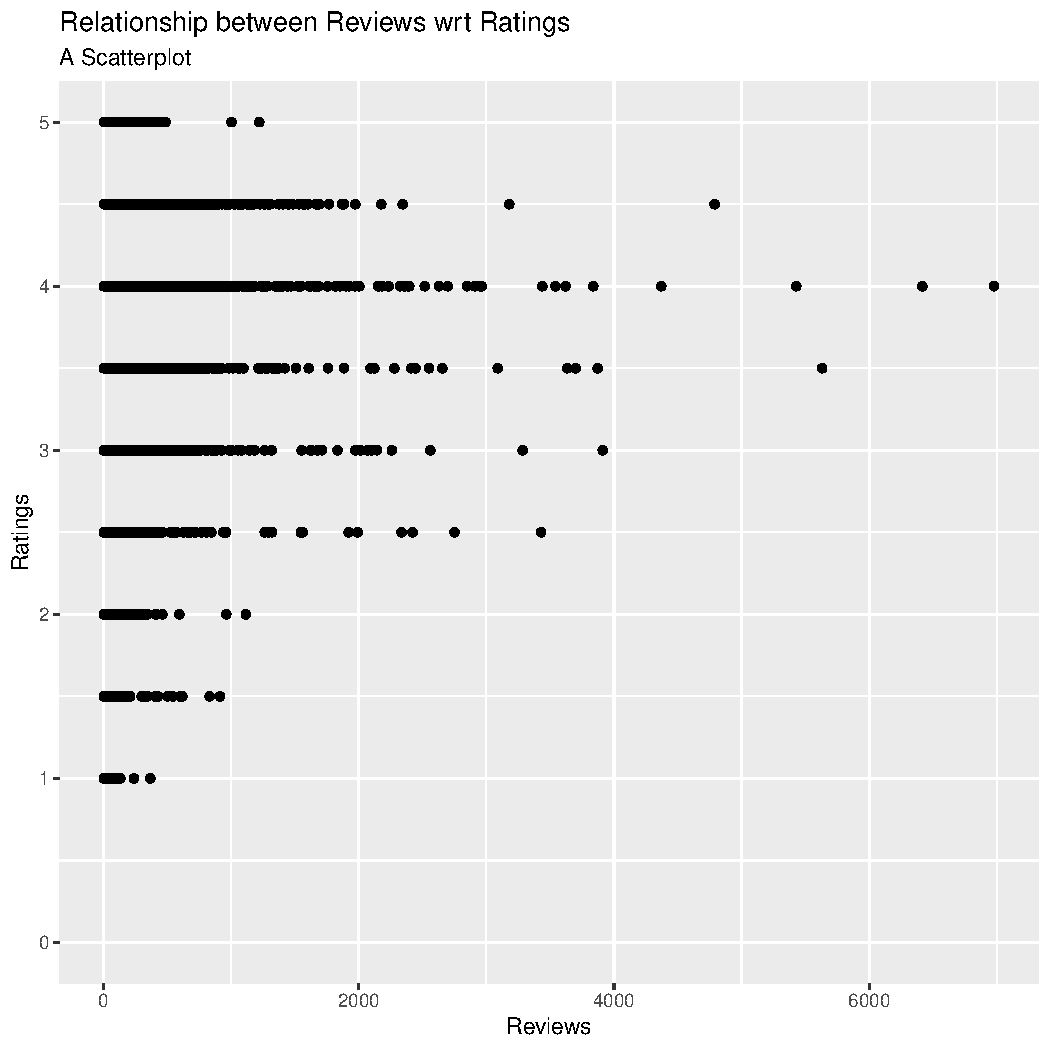
\includegraphics[width=\maxwidth]{figure/add_guides-1} 

\end{knitrout}

\begin{DIY}{Warning}
\noindent Adding guides to the visualization, implies adding  a title (Note the \emph{ggtitle()} function), labels (Note the \emph{xlab()} and \emph{ylab()} functions) and legends (Using the \emph{labs()} function) to the plot. 
\end{DIY}

\newpage
\noindent \textbf{\Large \underline{Step 5}}: {\Large Set \emph{Aesthetics} to the \emph{Geoms}} 
\begin{knitrout}
\definecolor{shadecolor}{rgb}{0.969, 0.969, 0.969}\color{fgcolor}\begin{kframe}
\begin{alltt}
\hlstd{graph} \hlkwb{<-} \hlstd{graph} \hlopt{+} \hlkwd{geom_point}\hlstd{(}\hlkwc{colour} \hlstd{=} \hlstr{"blue"}\hlstd{)}
\hlcom{## set the colour of the points in the plot}
\hlstd{graph}
\end{alltt}
\end{kframe}
\includegraphics[width=\maxwidth]{figure/setting_aesthetics-1} 

\end{knitrout}

\begin{DIY}{Warning}
\noindent  ggplot allows us to set the aesthetics of the \emph{geoms} as shown here. However, there is a difference between \textbf{aesthetics setting} and \textbf{aesthetics mapping}. What is demonstrated here is an example of aesthetics setting
\end{DIY}

\begin{DIY}{Homework}
\noindent  Pass aes(colour = "blue") as an argument to \emph{geom\textunderscore point()}. What do you observe?
\end{DIY}

\newpage
\noindent \textbf{\Large \underline{Step 6}}: {\Large Add \emph{Facets} to the visualization}
\begin{knitrout}
\definecolor{shadecolor}{rgb}{0.969, 0.969, 0.969}\color{fgcolor}\begin{kframe}
\begin{alltt}
\hlstd{graph} \hlopt{+} \hlkwd{facet_grid}\hlstd{( business}\hlopt{$}\hlstd{is_open} \hlopt{~} \hlstd{. )}
\end{alltt}
\end{kframe}
\includegraphics[width=\maxwidth]{figure/faceting-1} 
\begin{kframe}\begin{alltt}
\hlcom{## Visualize Reviews by open/closed status}
\end{alltt}
\end{kframe}
\end{knitrout}


\begin{DIY}{Homework}
\noindent Remove entries from the data frame that have reviews as NA. Moreover, add another column to the data frame that maps the is\textunderscore open values of "0" to "close" and "1" to "open". 
Finally, regenerate the plot, but now faceted on the new column. Name the new data frame as "cleansedBusiness" and the new column as "status\textunderscore char". 
\end{DIY}

\newpage


\newpage
\subsection{Generating a \textbf{\emph{Boxplot}}}
\noindent \textbf{\underline{Question}}: What is the distribution of ratings by status? 
\begin{knitrout}
\definecolor{shadecolor}{rgb}{0.969, 0.969, 0.969}\color{fgcolor}\begin{kframe}
\begin{alltt}
\hlstd{graph} \hlkwb{<-} \hlkwd{ggplot}\hlstd{( cleansedBusiness )} \hlcom{## attach the new df to plotting env}
\hlstd{interval} \hlkwb{<-} \hlkwd{seq}\hlstd{(} \hlnum{0}\hlstd{,} \hlkwd{max}\hlstd{(cleansedBusiness}\hlopt{$}\hlstd{stars),} \hlnum{0.5} \hlstd{)} \hlcom{## create a sequence }
\hlcom{## from 0 to max value of stars column with an increment value of 0.5}
\hlstd{graph} \hlkwb{<-} \hlstd{graph} \hlopt{+}
\hlkwd{aes}\hlstd{(} \hlkwc{x} \hlstd{= cleansedBusiness}\hlopt{$}\hlstd{status_char,}
     \hlcom{## map the new column to the x axis}
     \hlkwc{y} \hlstd{= cleansedBusiness}\hlopt{$}\hlstd{stars}
     \hlcom{## map the stars column to the y axis }
   \hlstd{)} \hlopt{+}
\hlkwd{geom_boxplot}\hlstd{(} \hlkwc{outlier.color} \hlstd{=} \hlstr{"red"} \hlstd{)} \hlopt{+}
\hlcom{##add geom to the plot in this case a box plot and set the colour of the }
\hlcom{##outlier values to red}
\hlkwd{ggtitle}\hlstd{(} \hlstr{"Distribution of Ratings by Status "}\hlstd{,} \hlkwc{subtitle} \hlstd{=} \hlstr{"Boxplot"} \hlstd{)} \hlopt{+}
\hlkwd{xlab}\hlstd{(} \hlstr{"Status"} \hlstd{)} \hlopt{+} \hlkwd{ylab}\hlstd{(} \hlstr{"Ratings"} \hlstd{)}  \hlcom{##add guides to the plot}
\hlstd{graph} \hlopt{+} \hlkwd{scale_y_continuous}\hlstd{(} \hlkwc{breaks} \hlstd{= interval )}
\end{alltt}
\end{kframe}
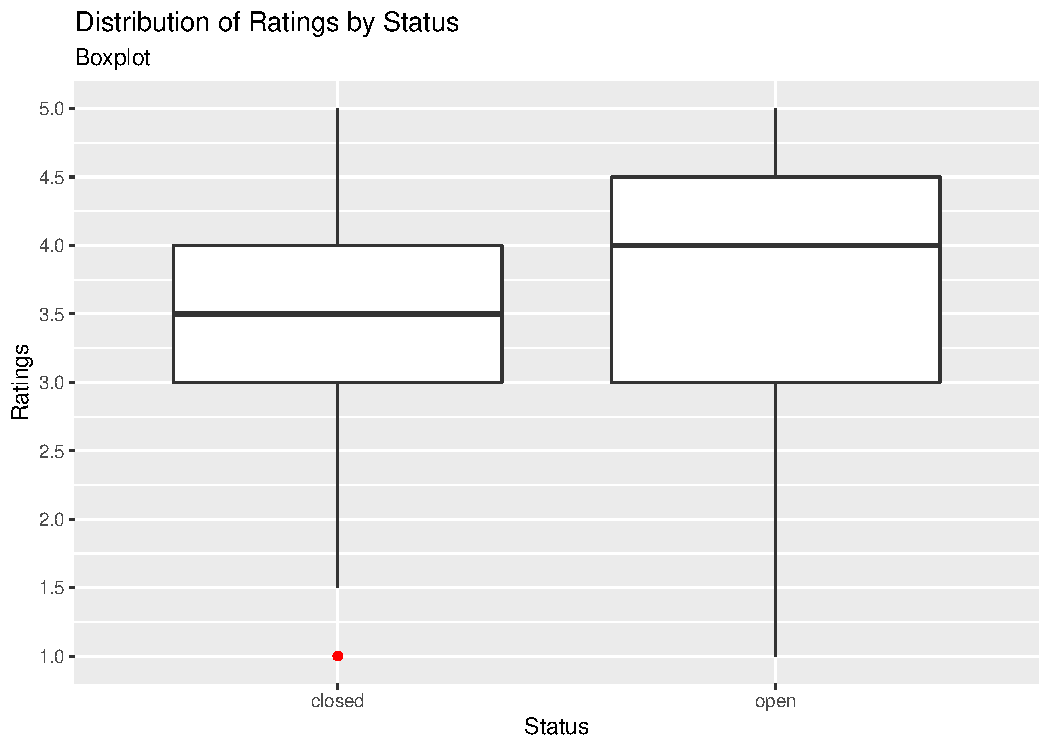
\includegraphics[width=\maxwidth]{figure/Boxplot-1} 
\begin{kframe}\begin{alltt}
\hlcom{##change the resolution of the y axis }
\end{alltt}
\end{kframe}
\end{knitrout}

\begin{DIY}{Warning}
\noindent Pay close attention the scale\textunderscore y\textunderscore continuous() function and the argument passed to it
\end{DIY}

\begin{DIY}{Warning}
\noindent Note the outlier$.$color parameter that is set and passed to geom\textunderscore boxplot  
\end{DIY}

\begin{DIY}{Think}
\noindent Read the help manual for scale\textunderscore x\textunderscore discrete() and argue why is scale\textunderscore y\textunderscore continuous() a better choice in this case.
\end{DIY}


\subsection{Generating a \textbf{\emph{Barplot}}}
\noindent \textbf{\underline{Question}}: What is the distribution of reviews? 
\begin{knitrout}
\definecolor{shadecolor}{rgb}{0.969, 0.969, 0.969}\color{fgcolor}\begin{kframe}
\begin{alltt}
\hlstd{graph} \hlkwb{<-}  \hlkwd{ggplot}\hlstd{(cleansedBusiness)} \hlcom{## add data to the viz environment}
\hlstd{graph} \hlopt{+}
\hlkwd{aes}\hlstd{(} \hlkwc{x} \hlstd{= cleansedBusiness}\hlopt{$}\hlstd{review_count )}  \hlopt{+}
\hlcom{## map the review count column to the x axis . Since its a bar plot, the }
\hlcom{## y axis is a count for each  element in the x axis  }
\hlkwd{geom_bar}\hlstd{()} \hlopt{+}
\hlcom{## add geom to the plot in this case a bar plot   }
\hlkwd{ggtitle}\hlstd{(} \hlstr{"Distribution of Review Count"}\hlstd{,}
         \hlkwc{subtitle} \hlstd{=} \hlstr{"A Barplot"} \hlstd{)} \hlopt{+}
\hlkwd{xlab}\hlstd{(}\hlstr{"Reviews"}\hlstd{)} \hlopt{+} \hlkwd{ylab}\hlstd{(}\hlstr{"Frequency"}\hlstd{)} \hlcom{# add guides to the viz environment}
\end{alltt}
\end{kframe}
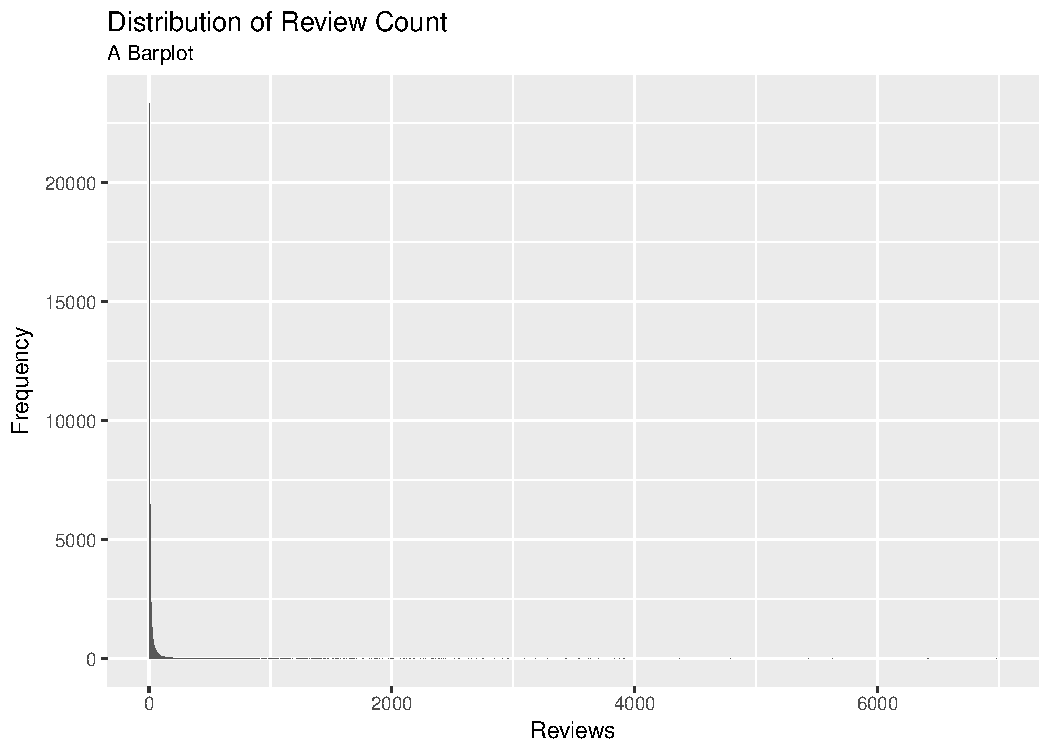
\includegraphics[width=\maxwidth]{figure/BarPlot-1} 

\end{knitrout}


\begin{DIY}{Homework}
\noindent Read the help manual for both geom\textunderscore bar()  and geom\textunderscore histogram().
Try using geom\textunderscore histogram() instead of geom\textunderscore bar(). Explain your observation.
\end{DIY}

\newpage
\subsection{Zooming into a Plot}
\noindent \textbf{\underline{Question}}: What is the distribution of reviews within the 3rd quartile?
\begin{knitrout}
\definecolor{shadecolor}{rgb}{0.969, 0.969, 0.969}\color{fgcolor}\begin{kframe}
\begin{alltt}
\hlstd{graph} \hlkwb{<-}  \hlkwd{ggplot}\hlstd{(cleansedBusiness)} \hlcom{## add data to the viz environment}
\hlstd{thirdQuartile} \hlkwb{<-} \hlkwd{summary}\hlstd{(cleansedBusiness}\hlopt{$}\hlstd{review_count)[}\hlnum{5}\hlstd{]}
\hlcom{## The third quartile of the review counts}
\hlstd{graph} \hlkwb{<-} \hlstd{graph} \hlopt{+}
\hlkwd{aes}\hlstd{(}\hlkwc{x} \hlstd{= cleansedBusiness}\hlopt{$}\hlstd{review_count)}  \hlopt{+}
 \hlcom{## map the review count column to the x axis . Since its a bar plot, }
\hlcom{## the y axis is a count for each  element in the x axis  }
\hlkwd{geom_bar}\hlstd{()} \hlopt{+}
\hlcom{## add geom to the plot in this case a bar plot   }
\hlkwd{ggtitle}\hlstd{(} \hlstr{"Distribution of Review Count"}\hlstd{,}
          \hlkwc{subtitle} \hlstd{=} \hlstr{"A Zommed In Barplot"} \hlstd{)} \hlopt{+}
\hlkwd{xlab}\hlstd{(} \hlstr{"Reviews"} \hlstd{)} \hlopt{+} \hlkwd{ylab}\hlstd{(} \hlstr{"Frequency"} \hlstd{)}
\hlcom{## add guides to the plot}
\hlstd{graph} \hlkwb{<-} \hlstd{graph} \hlopt{+}
\hlkwd{coord_cartesian}\hlstd{(} \hlkwc{xlim} \hlstd{=} \hlkwd{c}\hlstd{(}\hlnum{0}\hlstd{,thirdQuartile) )}  \hlcom{## scale the x axis by  }
\hlcom{## limiting it to  show values only till the third quartile}
\hlstd{graph}
\end{alltt}
\end{kframe}
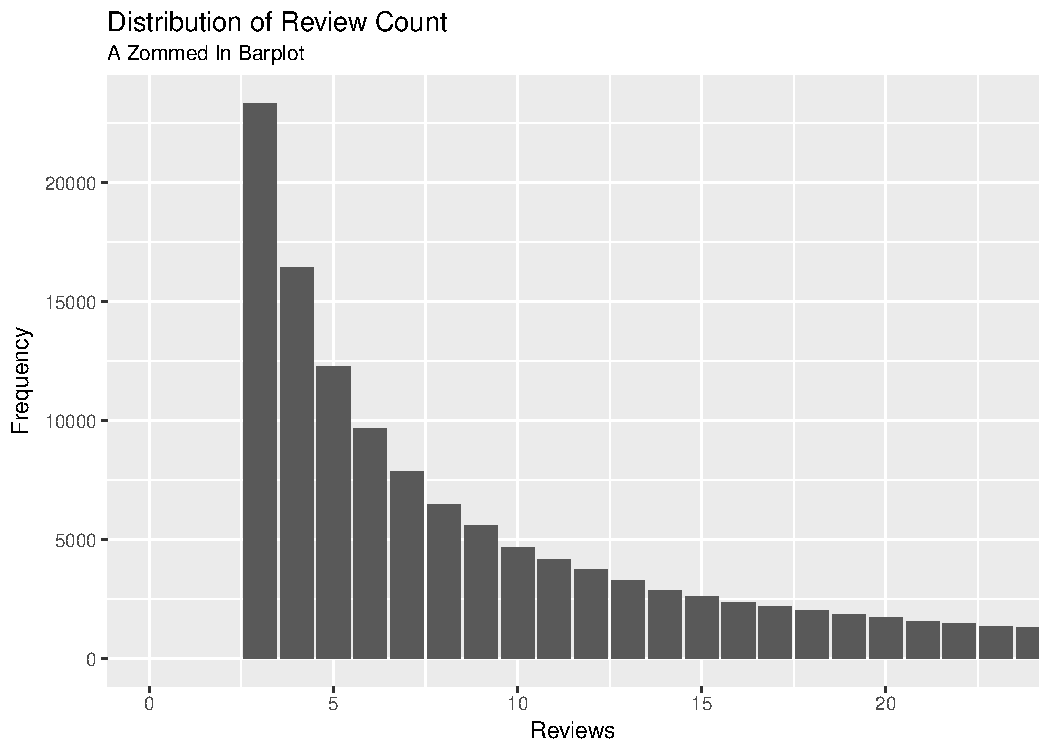
\includegraphics[width=\maxwidth]{figure/Zooming_In-1} 

\end{knitrout}

\begin{DIY}{Homework}
\noindent Read the help manual for both coord\textunderscore cartesian(). Try the above example without the coord\textunderscore cartesian() function. Explain your observation.
\end{DIY}

\newpage
\subsection{Changing Axis Resolution}
\noindent \textbf{\underline{Question}}: How do we change the resolution of the x axis to interval of 1?
\begin{knitrout}
\definecolor{shadecolor}{rgb}{0.969, 0.969, 0.969}\color{fgcolor}\begin{kframe}
\begin{alltt}
\hlstd{graph1} \hlkwb{<-} \hlstd{graph} \hlopt{+}
\hlkwd{scale_x_continuous}\hlstd{(}
                   \hlkwc{breaks} \hlstd{=} \hlkwd{seq}\hlstd{(}\hlnum{0}\hlstd{,thirdQuartile,}\hlnum{1}\hlstd{)}
                  \hlstd{)}  \hlcom{## change the resolution of the}
\hlcom{## x-axis to interval of 1}
\hlstd{graph1}
\end{alltt}
\end{kframe}
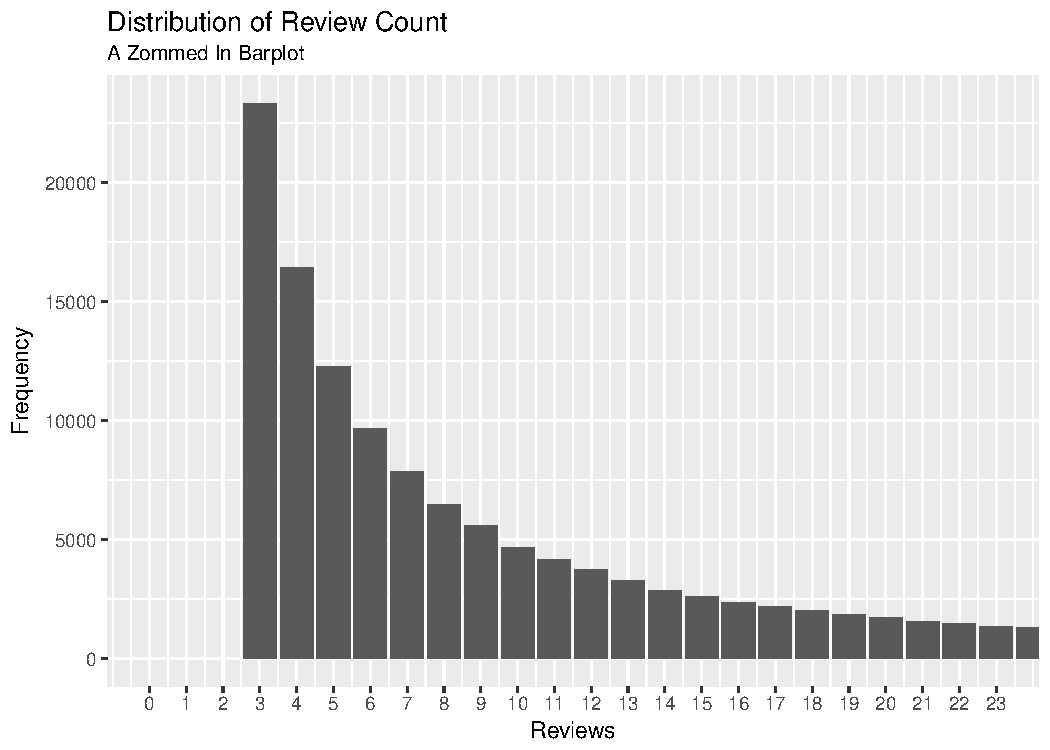
\includegraphics[width=\maxwidth]{figure/Change_Axis_Resolution-1} 

\end{knitrout}

\begin{DIY}{Homework}
\noindent Generate a box plot for the same data and with the same zoomed in view as the barplot
\end{DIY}




\newpage
\subsection{Generating Stacked Barplot and Dodged Barplot}
\noindent \textbf{\underline{Question}}: What is the distribution of reviews grouped by ratings?

\begin{knitrout}
\definecolor{shadecolor}{rgb}{0.969, 0.969, 0.969}\color{fgcolor}\begin{kframe}
\begin{alltt}
\hlstd{graph}    \hlkwb{<-}  \hlkwd{ggplot}\hlstd{(cleansedBusiness)} \hlcom{## Attach data to ggplot }
\hlstd{base_graph} \hlkwb{<-} \hlstd{graph} \hlopt{+}
\hlkwd{aes}\hlstd{(}\hlkwc{x} \hlstd{=}
      \hlstd{cleansedBusiness}\hlopt{$}\hlstd{review_count} \hlcom{## set the aesthetics by mapping }
\hlcom{## the  review count to the x axis}
    \hlstd{)} \hlopt{+}
\hlkwd{coord_cartesian}\hlstd{(}
            \hlkwc{xlim} \hlstd{=} \hlkwd{c}\hlstd{(}\hlnum{0}\hlstd{,thirdQuartile)} \hlcom{## scale the x axis by limiting }
\hlcom{##it to show values only till the third quartile}
             \hlstd{)}  \hlopt{+}
\hlkwd{scale_x_continuous}\hlstd{(}
           \hlkwc{breaks} \hlstd{=} \hlkwd{seq}\hlstd{(}\hlnum{0}\hlstd{,thirdQuartile,}\hlnum{1}\hlstd{)} \hlcom{## change the resolution of }
\hlcom{## the x-axis to interval of 1}
           \hlstd{)} \hlopt{+}
\hlkwd{xlab}\hlstd{(}\hlstr{"Reviews"}\hlstd{)} \hlopt{+} \hlkwd{ylab}\hlstd{(}\hlstr{"Frequency"}\hlstd{)} \hlcom{## add titles to the coordinate axes}
\hlstd{graph1} \hlkwb{<-} \hlstd{base_graph} \hlopt{+}
\hlkwd{geom_bar}\hlstd{(}
          \hlkwd{aes}\hlstd{(}\hlkwc{fill} \hlstd{=}
              \hlkwd{as.factor}\hlstd{(cleansedBusiness}\hlopt{$}\hlstd{stars)}
              \hlcom{## map groups of reviews by stars to the aesthetics of }
             \hlstd{)} \hlcom{## fill colour in segments of the bar plot by the  }
              \hlcom{## size of each group }
       \hlstd{)}  \hlopt{+}
\hlcom{## By default the bar plot is a stacked barplot }
\hlkwd{ggtitle}\hlstd{(} \hlstr{"Distribution of Review Count Per Rating"}\hlstd{,}
         \hlkwc{subtitle} \hlstd{=} \hlstr{"A Zoomed In Stacked Barplot Per State"}
       \hlstd{)} \hlcom{## add titles and subtitles}
\hlstd{graph2} \hlkwb{<-} \hlstd{base_graph} \hlopt{+}
\hlkwd{geom_bar}\hlstd{(}
         \hlkwd{aes}\hlstd{(}\hlkwc{fill} \hlstd{=}
                \hlkwd{as.factor}\hlstd{(cleansedBusiness}\hlopt{$}\hlstd{stars)}
            \hlstd{),}
         \hlkwc{position} \hlstd{=} \hlstr{"dodge"} \hlcom{## change the position argument of geom_bar() }
\hlcom{## to create a dodged bar plot where the height of each bar is }
\hlcom{## size of each   group }
        \hlstd{)} \hlopt{+}
\hlkwd{ggtitle}\hlstd{(} \hlstr{"Distribution of Review Count Per Rating"}\hlstd{,}
        \hlkwc{subtitle} \hlstd{=} \hlstr{"A Zoomed In Dodged BarPlot Per State"}\hlstd{)}
\hlstd{gridExtra}\hlopt{::}\hlkwd{grid.arrange}\hlstd{(}
              \hlstd{graph1} \hlopt{+} \hlkwd{labs}\hlstd{(}\hlkwc{fill} \hlstd{=} \hlstr{"Rating"}\hlstd{),}
              \hlstd{graph2} \hlopt{+} \hlkwd{labs}\hlstd{(}\hlkwc{fill} \hlstd{=} \hlstr{"Rating"}\hlstd{),} \hlcom{##The labs() function }
\hlcom{## sets the labels of the plot. Note that we set the argument fill to  }
\hlcom{## the label name as that is the same argument we have used in aes().}
              \hlkwc{nrow} \hlstd{=} \hlnum{2}
            \hlstd{)}  \hlcom{## generate both plots together. The nrow parameter }
\end{alltt}
\end{kframe}
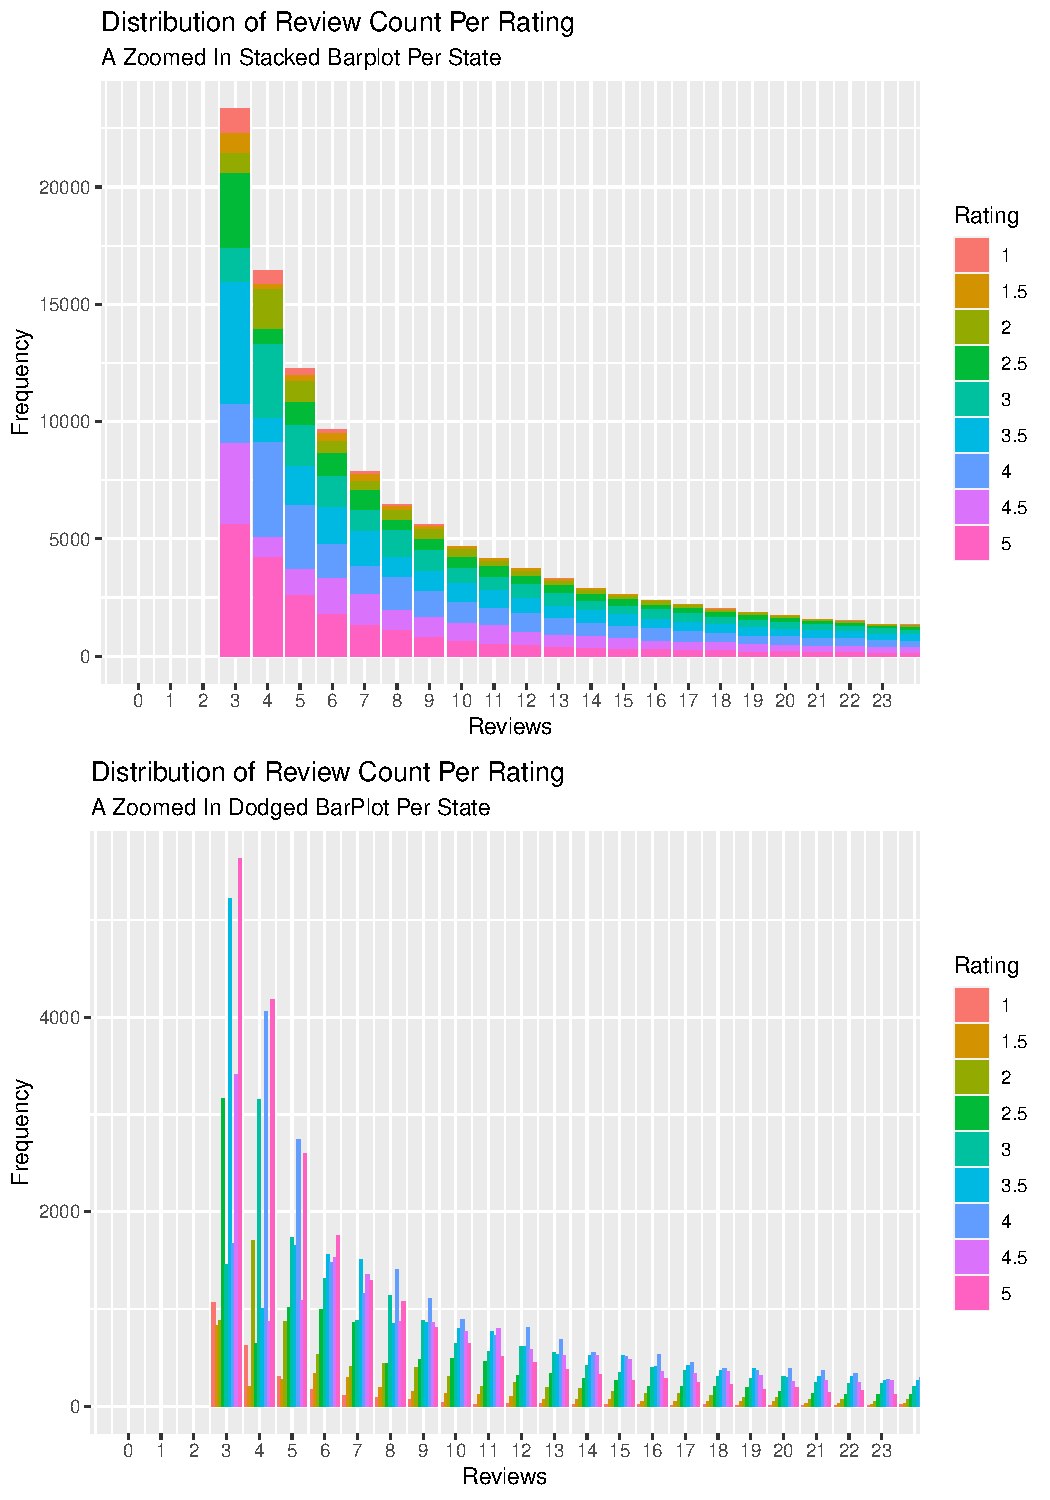
\includegraphics[width=\maxwidth]{figure/Aesthetics_Mapping-1} 
\begin{kframe}\begin{alltt}
\hlcom{## specifies the row-wise split of the visual environment. }
\end{alltt}
\end{kframe}
\end{knitrout}

\begin{DIY}{Warning}
\begin{itemize}
  \item \noindent Note the outlier$.$color parameter that is set and passed to geom\textunderscore boxplot
  \item \noindent Note the use of \textbf{aesthetic mapping} when aes() is passed as an argument to geom\textunderscore bar()
  \item \noindent Node the use of labs() to set the legend of the plot
\end{itemize}
\end{DIY}

\begin{DIY}{Think}
\noindent  What would be the outcome if we used geom\textunderscore histogram() instead of geom\textunderscore bar() 
\end{DIY}

\begin{DIY}{Think}
\noindent  Why did we pass the argument \emph{fill} to the labs() function. What would be the outcome if we passed \emph{colour} instead?
\end{DIY}

\begin{DIY}{Homework}
\noindent Read the help manual for grid$.$arrange() function.
\end{DIY}

\newpage
\subsection{Merging Data Frames}
\noindent \textbf{\underline{Question}}: How can we create a data frame of businesses in top10 categoriesm, having an additional attribute called "category"?
\begin{knitrout}
\definecolor{shadecolor}{rgb}{0.969, 0.969, 0.969}\color{fgcolor}\begin{kframe}
\begin{alltt}
\hlstd{countPerCategory} \hlkwb{<-} \hlkwd{aggregate}\hlstd{( category}\hlopt{$}\hlstd{category ,}
                               \hlkwc{by} \hlstd{=} \hlkwd{list}\hlstd{(category}\hlopt{$}\hlstd{category),}
                               \hlkwc{FUN} \hlstd{= length}
                              \hlstd{)} \hlcom{## group the categories in the category }
\hlcom{##data setby their count}
\hlkwd{names}\hlstd{(countPerCategory)} \hlkwb{<-} \hlkwd{c}\hlstd{(}\hlstr{"category"}\hlstd{,}\hlstr{"count"}\hlstd{)}
\hlcom{## add names to the resulting data frame}
\hlstd{top10Categories} \hlkwb{<-} \hlkwd{head}\hlstd{(}
                        \hlstd{countPerCategory[}
                        \hlkwd{order}\hlstd{(countPerCategory}\hlopt{$}\hlstd{count,}
                              \hlkwc{decreasing} \hlstd{=} \hlnum{TRUE}\hlstd{),}
                        \hlcom{## order the countPerCategory data frame in}
                        \hlcom{## decreasing order}
                       \hlstd{],}
                       \hlkwc{n}\hlstd{=}\hlnum{10} \hlcom{## list only the top 10 elements in the }
                       \hlcom{## sorted data frame}
                      \hlstd{)}
\hlstd{businesses_top10Categories} \hlkwb{<-}
\hlstd{category[}
          \hlstd{category}\hlopt{$}\hlstd{category}
          \hlopt
          \hlstd{top10Categories[,}\hlnum{1}\hlstd{],} \hlcom{## search for matching category }
          \hlcom{## in the category dataframe and list all   }
          \hlcom{## matching entries in category}
      \hlstd{]}

\hlstd{businesses_top10Merged} \hlkwb{<-} \hlkwd{merge}\hlstd{( cleansedBusiness,}
                          \hlstd{businesses_top10Categories,}
                          \hlkwc{by.x} \hlstd{=} \hlstr{"id"}\hlstd{,}\hlkwc{by.y} \hlstd{=} \hlstr{"business_id"}
                        \hlstd{)}
\hlcom{## merging two data frames  by business id}
\end{alltt}
\end{kframe}
\end{knitrout}

\begin{DIY}{Homework}
\noindent Read the help manual for merge() function.
\end{DIY}

\newpage
\subsection{Generating a \textbf{\emph{Densityplot}}}
\noindent \textbf{\underline{Question}}: What is the distribution of ratings for each of the top 10 most frequent categories?

\begin{knitrout}
\definecolor{shadecolor}{rgb}{0.969, 0.969, 0.969}\color{fgcolor}\begin{kframe}
\begin{alltt}
\hlstd{graph} \hlkwb{<-} \hlkwd{ggplot}\hlstd{(businesses_top10Merged)} \hlcom{## attached the merged dataframe }
\hlcom{## to the viz environment. This new new data frame contains only businesses}
\hlcom{## belonging to the top 10 categories and has an additional column called }
\hlcom{## category}
\hlstd{base_graph} \hlkwb{<-} \hlstd{graph} \hlopt{+}
\hlkwd{aes}\hlstd{(} \hlkwc{x} \hlstd{= businesses_top10Merged}\hlopt{$}\hlstd{stars} \hlcom{## map the attrbute stars to the }
     \hlcom{## x axis}
   \hlstd{)}  \hlopt{+}
\hlkwd{xlab}\hlstd{(}\hlstr{"Ratings"}\hlstd{)} \hlopt{+}
\hlkwd{ylab}\hlstd{(}\hlstr{" Normalized Frequency"}\hlstd{)} \hlopt{+}
\hlkwd{ggtitle}\hlstd{(}\hlstr{"Distribution of Ratings Per Frequent Category"}\hlstd{,}
        \hlkwc{subtitle} \hlstd{=} \hlstr{"A Histogram"}\hlstd{)}
\hlcom{## added guides to the visualization}
\hlstd{graph1} \hlkwb{<-} \hlstd{base_graph} \hlopt{+}
\hlkwd{geom_histogram}\hlstd{(}
                 \hlkwd{aes}\hlstd{(}
                      \hlkwc{y} \hlstd{= ..count..} \hlopt{/} \hlkwd{sum}\hlstd{(..count..),}
                      \hlcom{## geom_histogram() contains an outcome variable }
                      \hlcom{## called count "..count.." tells geom_histogram()}
                      \hlcom{## to refer to its own outcome variable oand not treat }
                      \hlcom{## count as a user defined variable. Here, we are mapping }
                      \hlcom{## the frequency of each element in the x-axis to y-axis }
                      \hlkwc{fill} \hlstd{= businesses_top10Merged}\hlopt{$}\hlstd{category}
                      \hlcom{## groups the y-values by category and maps it to the }
                      \hlcom{## the aesthetics of filling colour in }
                      \hlcom{## segments of the plot by the  size of}
                      \hlcom{## each group}
                    \hlstd{)}
              \hlstd{)} \hlopt{+}
\hlkwd{labs}\hlstd{(} \hlkwc{fill} \hlstd{=} \hlstr{"Categories"} \hlstd{)}  \hlcom{#The labs() function sets }
\hlcom{## the labels of the plot. Note that we set the argument fill to  }
\hlcom{## the label name as that is the same argument we have used in aes().}
\hlstd{graph2} \hlkwb{<-} \hlstd{base_graph} \hlopt{+}
\hlkwd{geom_density}\hlstd{(}
              \hlkwd{aes}\hlstd{(}\hlkwc{color} \hlstd{=}
                    \hlkwd{as.factor}\hlstd{(businesses_top10Merged}\hlopt{$}\hlstd{category)}
                \hlstd{)} \hlcom{## groups the y-values by category and maps it to the }
                  \hlcom{## the aesthetics of colouring each }
                  \hlcom{## density function by category. }
           \hlstd{)} \hlopt{+}
 \hlcom{##the density plot based on the top10 categories}
\hlkwd{labs}\hlstd{(} \hlkwc{color} \hlstd{=} \hlstr{"Categories"} \hlstd{)} \hlcom{##setting the label}
\hlcom{## to categories. Please note the use setting of the }
\hlcom{## color aesthetics since we did the same in geom_density}
\hlstd{gridExtra}\hlopt{::}\hlkwd{grid.arrange}\hlstd{(}
                        \hlstd{graph1 ,graph2,}
                       \hlkwc{nrow} \hlstd{=} \hlnum{2}\hlstd{)}\hlcom{## generate both plots together. }
\end{alltt}


{\ttfamily\noindent\itshape\color{messagecolor}{\#\# `stat\_bin()` using `bins = 30`. Pick better value with `binwidth`.}}\end{kframe}
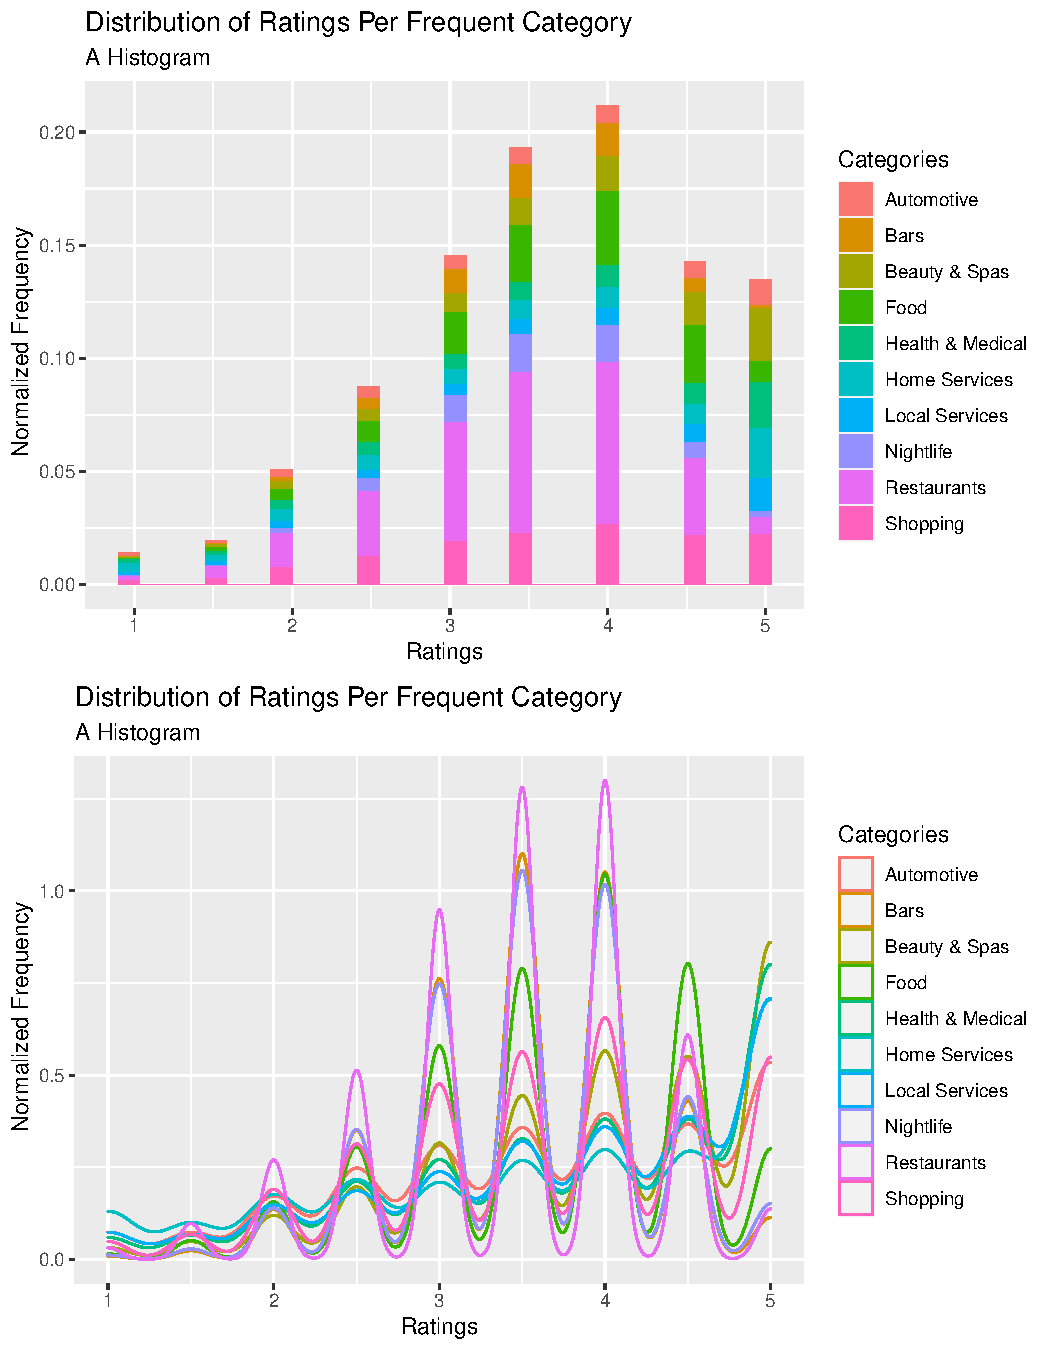
\includegraphics[width=\maxwidth]{figure/unnamed-chunk-38-1} 
\begin{kframe}\begin{alltt}
\hlcom{## The nrow parameter specifies the row-wise split }
\hlcom{## of the visual environment. }
\end{alltt}
\end{kframe}
\end{knitrout}

\begin{DIY}{Think}
\noindent Note that for geom\textunderscore density() we map the "color" aesthetics instead of the 
"fill" aesthetics. Try mapping the "fill" aesthetics instead. What do you observe?
\end{DIY}

\subsection{Smoothing Density Plots}
\noindent \textbf{\underline{Question}}: How does the density estimate change under different smoothing parameters?
\begin{knitrout}
\definecolor{shadecolor}{rgb}{0.969, 0.969, 0.969}\color{fgcolor}\begin{kframe}
\begin{alltt}
\hlstd{base_graph} \hlopt{+} \hlkwd{geom_line}\hlstd{(} \hlkwc{stat} \hlstd{=} \hlstr{"density"} \hlstd{)} \hlopt{+} \hlcom{## geom_line() connects the }
\hlcom{## data in their order along the x-axis. Moreover setting the stat argument }
\hlcom{## tells ggplot to create a density plot}
\hlkwd{geom_line}\hlstd{(} \hlkwc{stat} \hlstd{=} \hlstr{"density"}\hlstd{,} \hlkwc{colour} \hlstd{=} \hlstr{"red"}\hlstd{,} \hlkwc{adjust} \hlstd{=} \hlnum{0.5} \hlstd{)} \hlopt{+} \hlcom{## the adjust }
\hlcom{## parameter sets the smoothing factor of the density estimate}
\hlkwd{geom_line}\hlstd{(} \hlkwc{stat} \hlstd{=} \hlstr{"density"}\hlstd{,} \hlkwc{colour} \hlstd{=} \hlstr{"green"}\hlstd{,} \hlkwc{adjust} \hlstd{=} \hlnum{1.5} \hlstd{)} \hlopt{+}
\hlkwd{geom_line}\hlstd{(} \hlkwc{stat} \hlstd{=} \hlstr{"density"}\hlstd{,} \hlkwc{colour} \hlstd{=} \hlstr{"blue"}\hlstd{,} \hlkwc{adjust} \hlstd{=} \hlnum{0.75} \hlstd{)} \hlopt{+}
\hlkwd{geom_line}\hlstd{(} \hlkwc{stat} \hlstd{=} \hlstr{"density"}\hlstd{,} \hlkwc{colour} \hlstd{=} \hlstr{"yellow"}\hlstd{,} \hlkwc{adjust} \hlstd{=} \hlnum{1.75} \hlstd{)} \hlopt{+}
\hlkwd{facet_grid}\hlstd{(}
            \hlkwd{as.factor}\hlstd{( businesses_top10Merged}\hlopt{$}\hlstd{category )} \hlopt{~} \hlstd{.}
            \hlcom{## generates a density plot per category}
          \hlstd{)} \hlopt{+}
\hlkwd{labs}\hlstd{(} \hlkwc{caption} \hlstd{=} \hlstr{"Black(adjust = 1); Red(adjust = 0.5); 
                Green(adjust = 0.5); Blue(adjust = 0.5); 
                Yellow(adjust = 0.5)"}
    \hlstd{)}  \hlcom{## adds a caption to the plot }
\end{alltt}
\end{kframe}
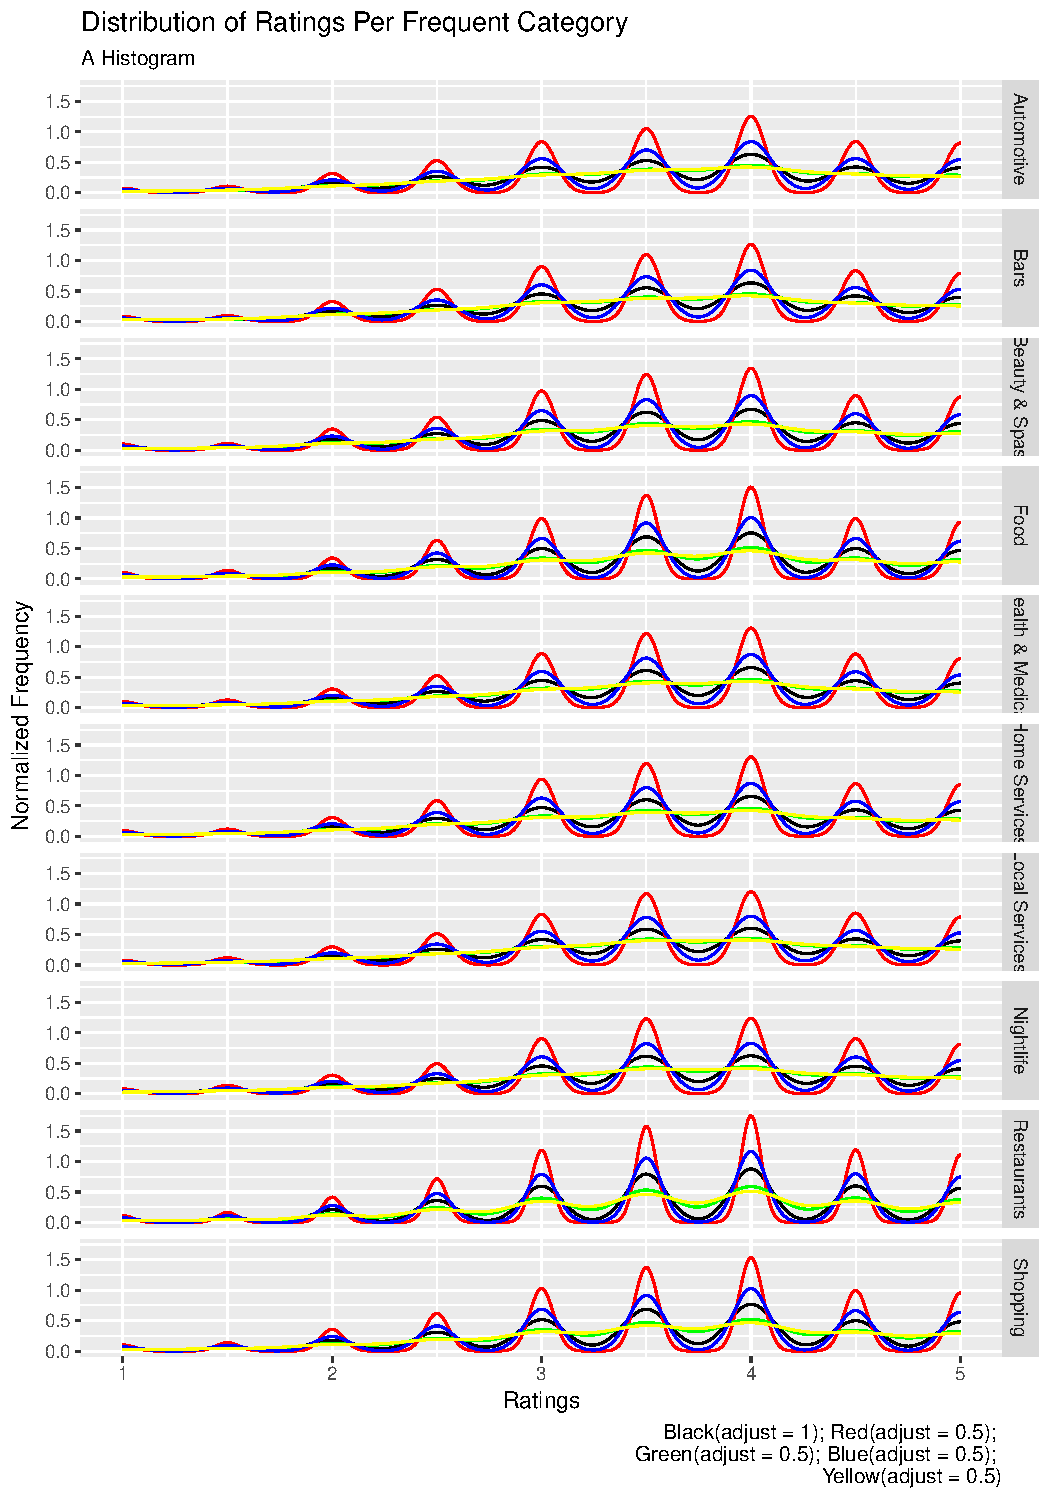
\includegraphics[width=\maxwidth]{figure/Faceted_Density_Plot-1} 

\end{knitrout}

\subsection{Combining Multiple Plots}
\subsubsection{Centering and Scaling the Data}
\label{sec:centering}
\begin{HIGHLIGHT}
\par\noindent{
{\centering{\textbf{\emph{\Large $\frac{X - \mu} {\sigma}$}}} \\} 
\noindent where $X$ is an observation in the dataset, $\mu$ and $\sigma$ are the mean and standard deviation respectively.
}
\end{HIGHLIGHT}
\begin{knitrout}
\definecolor{shadecolor}{rgb}{0.969, 0.969, 0.969}\color{fgcolor}\begin{kframe}
\begin{alltt}
\hlstd{centered} \hlkwb{<-} \hlstd{( businesses_top10Merged}\hlopt{$}\hlstd{stars}  \hlopt{-}
                \hlkwd{mean}\hlstd{( businesses_top10Merged}\hlopt{$}\hlstd{stars )}
              \hlcom{## compute the difference between each value in the stats}
              \hlcom{## attrbute and its mean}
             \hlstd{)} \hlopt{/} \hlkwd{sd}\hlstd{( businesses_top10Merged}\hlopt{$}\hlstd{stars )} \hlcom{## divide the difference}
            \hlcom{## by the standard deviation of stars  }
\hlstd{businesses_top10Merged} \hlkwb{<-} \hlkwd{data.frame}\hlstd{( businesses_top10Merged ,}
                                \hlkwc{centered_ratings} \hlstd{= centered )}
\end{alltt}
\end{kframe}
\end{knitrout}


\begin{DIY}{Homework}
\noindent Try centering the review attribute and generate two boxplots ,arranged side by side. The first boxplot should be on the uncentered review counts while the second boxplot
should be on the centered review counts. Explain your observation.
\end{DIY}

\noindent \textbf{\underline{Question}}:What is the distribution of Ratings once it has been centered?
\begin{knitrout}
\definecolor{shadecolor}{rgb}{0.969, 0.969, 0.969}\color{fgcolor}\begin{kframe}
\begin{alltt}
\hlstd{graph} \hlkwb{<-} \hlkwd{ggplot}\hlstd{( businesses_top10Merged )}
\hlstd{graph1} \hlkwb{<-} \hlstd{graph} \hlopt{+}
\hlkwd{aes}\hlstd{(} \hlkwc{x} \hlstd{= businesses_top10Merged}\hlopt{$}\hlstd{centered_ratings ,}
     \hlcom{## map centered_rating attribute to the x-axis }
     \hlkwc{y} \hlstd{= ..density..} \hlcom{##map the density variable of }
     \hlcom{## geom_density() to the y-axis }
   \hlstd{)} \hlopt{+}
\hlkwd{geom_histogram}\hlstd{(}\hlkwd{aes}\hlstd{(} \hlkwc{y} \hlstd{=}
                       \hlstd{..count..} \hlopt{/} \hlkwd{sum}\hlstd{(..count..)}
                    \hlcom{## count is the computed variable of }
                    \hlcom{## geom_histogram()}
                  \hlstd{)}
              \hlstd{)} \hlopt{+}
\hlkwd{geom_density}\hlstd{(} \hlkwc{adjust} \hlstd{=} \hlnum{4} \hlstd{)} \hlopt{+} \hlcom{## adjust the smoothness }
\hlcom{## of the density plot}
\hlkwd{xlab}\hlstd{(} \hlstr{"Centered Ratings"} \hlstd{)} \hlopt{+} \hlkwd{ylab}\hlstd{(} \hlstr{"Density"} \hlstd{)} \hlopt{+}
\hlkwd{ggtitle}\hlstd{(} \hlstr{"Distribution of Scaled Ratings"} \hlstd{)}  \hlcom{## add}
\hlcom{## guides to the plot}
\hlstd{graph1}
\end{alltt}


{\ttfamily\noindent\itshape\color{messagecolor}{\#\# `stat\_bin()` using `bins = 30`. Pick better value with `binwidth`.}}\end{kframe}
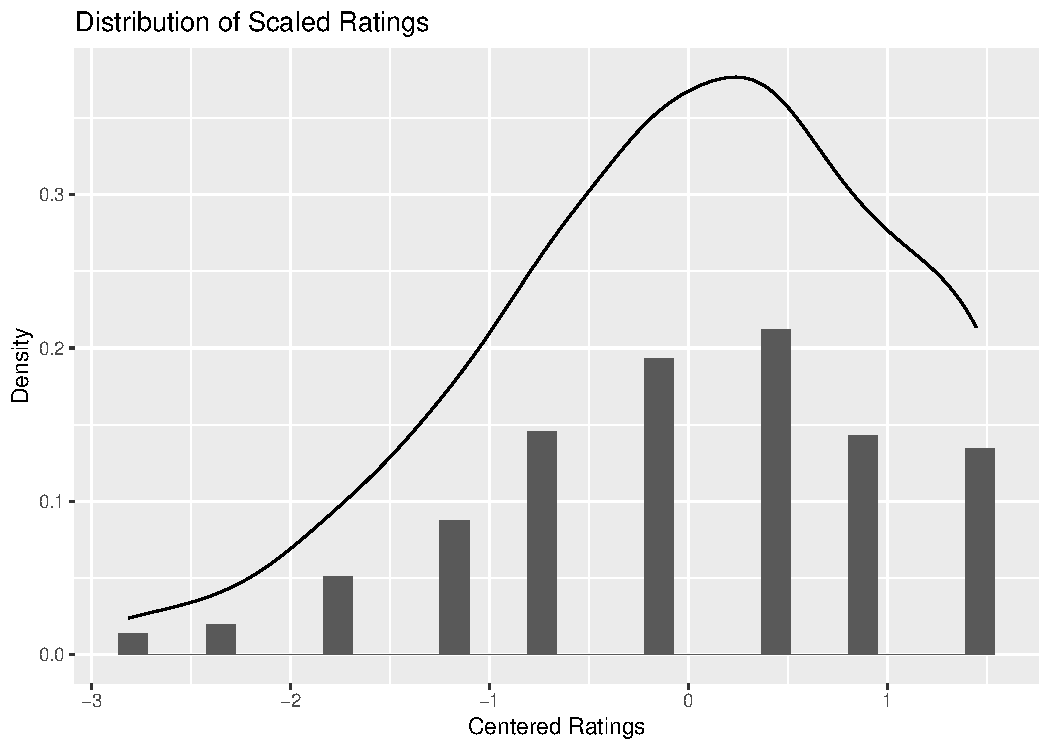
\includegraphics[width=\maxwidth]{figure/Centering_Ratings-1} 

\end{knitrout}

\subsection{Generating a \emph{\textbf{Columnplot}}}
\noindent \textbf{\underline{Question}}:What is the distribution of data Ratings per top 10 category, once it has been centered?
\begin{knitrout}
\definecolor{shadecolor}{rgb}{0.969, 0.969, 0.969}\color{fgcolor}\begin{kframe}
\begin{alltt}
\hlstd{rating_categorization} \hlkwb{<-} \hlkwd{ifelse}\hlstd{(}
                            \hlstd{businesses_top10Merged}\hlopt{$}\hlstd{centered_ratings} \hlopt{>} \hlnum{0}\hlstd{,}
                            \hlstr{"Above"}\hlstd{,}\hlstr{"Below"}\hlstd{)}
\hlcom{## Note the use of the ifelse statement, which checks if the }
\hlcom{## centered ratings are above or be low 0 and creates a vector}
\hlcom{## of containing "Above" / "Below"}
\hlstd{businesses_top10Merged} \hlkwb{<-} \hlkwd{data.frame}\hlstd{(businesses_top10Merged,}
  \hlkwc{rating_categorization} \hlstd{=}
          \hlstd{rating_categorization )} \hlcom{## add the new attribute to}
\hlcom{## the business_top10Merged data frame}
\hlstd{graph} \hlkwb{<-} \hlkwd{ggplot}\hlstd{(businesses_top10Merged)}
\hlstd{graph} \hlopt{+} \hlkwd{aes}\hlstd{(}\hlkwc{x} \hlstd{=} \hlkwd{as.factor}\hlstd{(}
                           \hlstd{businesses_top10Merged}\hlopt{$}\hlstd{category}
                          \hlstd{),}
                \hlcom{## map the x-axis to the category }
                \hlcom{## attribute of the businesses_top10Merged}
                \hlcom{## data frame}
           \hlkwc{y} \hlstd{=  businesses_top10Merged}\hlopt{$}\hlstd{centered_ratings )}  \hlopt{+}
                \hlcom{## map the y-axis to the centered_ratings}
                \hlcom{## attribute of the businesses_top10Merged df}
\hlkwd{geom_col}\hlstd{(} \hlkwd{aes}\hlstd{(} \hlkwc{fill} \hlstd{=}
                \hlkwd{as.factor}\hlstd{(businesses_top10Merged}\hlopt{$}\hlstd{rating_categorization)}
             \hlstd{)} \hlcom{## set the aesthetics mapping to group the business}
          \hlcom{## categories by whether they are "Above" / "Below".}
        \hlstd{)} \hlopt{+}
\hlkwd{theme}\hlstd{(} \hlkwc{axis.text.y} \hlstd{=} \hlkwd{element_blank}\hlstd{() )} \hlopt{+}
\hlcom{## Disable the labels on the y-axis }
\hlkwd{labs}\hlstd{(} \hlkwc{fill} \hlstd{=} \hlstr{"Rating"} \hlstd{)} \hlopt{+}
\hlkwd{xlab}\hlstd{(}\hlstr{"Category"}\hlstd{)} \hlopt{+} \hlkwd{ylab}\hlstd{(}\hlstr{"Distribution of Rating"}\hlstd{)} \hlopt{+}
\hlkwd{ggtitle}\hlstd{(}\hlstr{"Distribution of Ratings per Category"}\hlstd{)} \hlcom{## add guides to the }
\end{alltt}
\end{kframe}
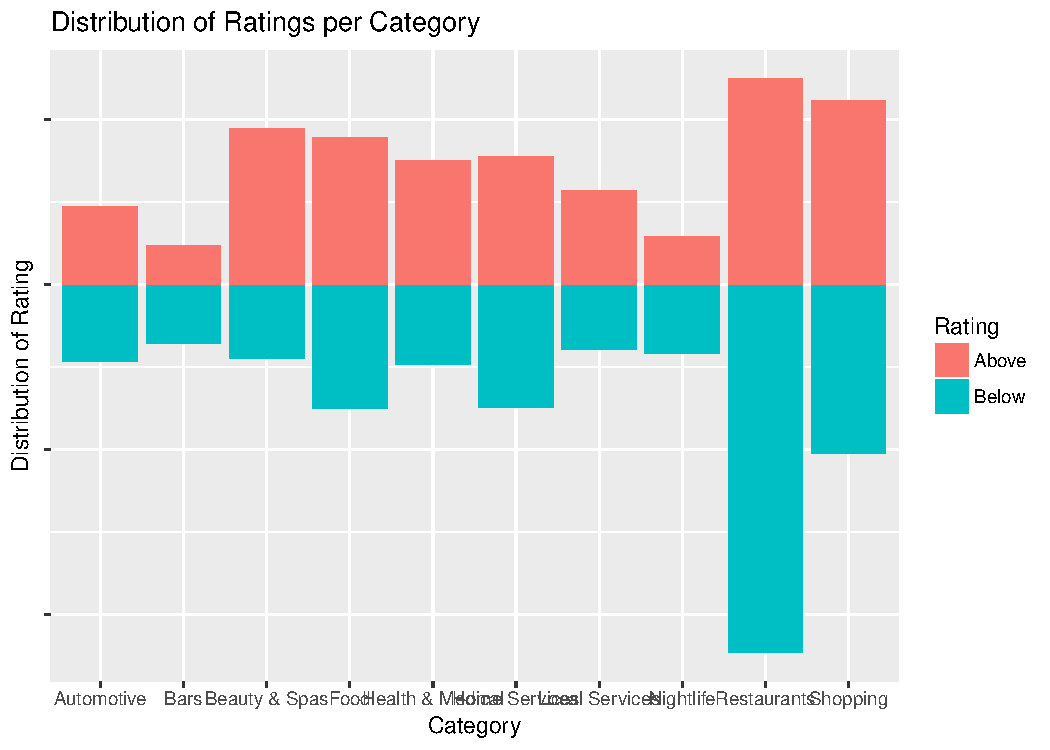
\includegraphics[width=\maxwidth]{figure/Column_Plot-1} 
\begin{kframe}\begin{alltt}
\hlcom{## plot}
\end{alltt}
\end{kframe}
\end{knitrout}






% !Rnw root = main.Rnw
\newpage
%======================================
\section{Statistical Modeling}
%======================================
%==================================================================
\subsection{Binary Vector Representation of Categorical Attributes}
%==================================================================
As explained in \ref{sec:GeomOfData}, each categorical value needs to be mapped to a different dimension. This requires us to represent categorical values as a binary vector.\\

\noindent \textbf{\underline{Question}}: What is the binary vector representation of the top10 categories?
\begin{knitrout}
\definecolor{shadecolor}{rgb}{0.969, 0.969, 0.969}\color{fgcolor}\begin{kframe}
\begin{alltt}
\hlcom{## a function to create a binary vector }
\hlcom{## the function accepts the following arguments}
\hlcom{## category_ =  a category of type character whose corresponding position}
\hlcom{##   in the binary vector is set to TRUE}
\hlcom{## categoryNames_ = a vector of category names that defines the }
\hlcom{##   total number of categories and hence the output dimension}
\hlcom{## returns: a vector of type logical which has dimensions  }
\hlcom{##            length(categoryNames_) x 1}
\hlstd{createBinaryCategoryVector} \hlkwb{<-} \hlkwa{function}\hlstd{(}\hlkwc{category_}\hlstd{,}\hlkwc{categoryNames_}\hlstd{)\{}
  \hlstd{colIdx} \hlkwb{<-} \hlkwd{which}\hlstd{(categoryNames_} \hlopt{==} \hlstd{category_)}
  \hlcom{## find the index of the categoryNames_ vector that }
  \hlcom{## matches the value in category_. The logical value}
  \hlcom{## for this position has to be set to TRUE}
  \hlstd{leftVec} \hlkwb{<-} \hlkwd{rep} \hlstd{(} \hlnum{FALSE}\hlstd{,(colIdx}\hlopt{-}\hlnum{1}\hlstd{) )}
  \hlcom{## create a vector for the left of the matching position}
  \hlstd{rightVec} \hlkwb{<-} \hlkwd{rep} \hlstd{(} \hlnum{FALSE}\hlstd{,} \hlkwd{length}\hlstd{(categoryNames_)} \hlopt{-} \hlstd{colIdx )}
  \hlcom{## create a vector for the right of the matching position}
  \hlstd{categoryVec} \hlkwb{<-} \hlkwd{c}\hlstd{(leftVec,} \hlnum{TRUE}\hlstd{, rightVec)}
  \hlcom{##concatenate the left and right vectors to the value  }
  \hlkwd{return}\hlstd{(categoryVec)}
\hlstd{\}}

\hlstd{CategoriesCount} \hlkwb{<-} \hlkwd{aggregate}\hlstd{(category}\hlopt{$}\hlstd{category,}
                             \hlkwc{by} \hlstd{=} \hlkwd{list}\hlstd{(category}\hlopt{$}\hlstd{category),}
                             \hlstd{length)}
\hlcom{## find the fereency of occurence of each category from the }
\hlcom{## category dataset}
\hlkwd{names}\hlstd{(CategoriesCount)} \hlkwb{<-} \hlkwd{c}\hlstd{(}\hlstr{"category"}\hlstd{,}\hlstr{"frequency"}\hlstd{)}
\hlcom{## assign attribute names to the CategoriesCount df }
\hlstd{mostFrequentCategories} \hlkwb{<-} \hlkwd{head}\hlstd{(}
                            \hlstd{CategoriesCount[}
                                          \hlkwd{order}\hlstd{(CategoriesCount}\hlopt{$}\hlstd{frequency,}
                                                \hlkwc{decreasing} \hlstd{=} \hlnum{TRUE}\hlstd{),}
                                        \hlstd{],}
                            \hlcom{## order the CategoriesCount dataframe in }
                            \hlcom{## decreasing order of occurence of}
                            \hlcom{## each category}
                            \hlkwc{n} \hlstd{=} \hlnum{10}
                        \hlstd{)}
\hlcom{##  get the 10 most frequent categories}
\hlstd{business_mostFrequentCategories} \hlkwb{<-} \hlstd{category[}
                                            \hlstd{category}\hlopt{$}\hlstd{category} \hlopt
                                            \hlstd{mostFrequentCategories}\hlopt{$}\hlstd{category,}
                                           \hlstd{]}
\hlcom{## get all business id's belonging to the top 10 categories}

\hlcom{## length(unique(business_mostFrequentCategories$business_id)) < }
\hlcom{##    length(business_mostFrequentCategories$business_id)}
\hlcom{## check if businesses are assigned to more than one category}

\hlstd{categoryMatrix} \hlkwb{<-} \hlkwd{t}\hlstd{(}
                      \hlkwd{sapply}\hlstd{(business_mostFrequentCategories}\hlopt{$}\hlstd{category,}
                            \hlkwc{FUN}\hlstd{=createBinaryCategoryVector,}
                            \hlkwc{categoryNames_}\hlstd{=mostFrequentCategories}\hlopt{$}\hlstd{category}
                          \hlstd{)}
                  \hlstd{)}
\hlcom{## for every value in business_mostFrequentCategories$category apply }
\hlcom{## the function createBinaryCategoryVector()  and transpose it to get }
\hlcom{## a binary vector of dimension }
\hlcom{## 1 X length(mostFrequentCategories$category)}
\hlcom{## Thefore for all applying the function to all elements of }
\hlcom{## business_mostFrequentCategories$category will  }
\hlcom{## result in a matrix of dimension:}
\hlcom{## length(business_mostFrequentCategories$category)  X }
\hlcom{##      length(mostFrequentCategories$category)}

\hlkwd{row.names}\hlstd{(categoryMatrix)} \hlkwb{<-} \hlkwa{NULL}
\hlcom{## set the row names of the category matrix to NULL to remove}
\hlcom{## duplicate row names as conversion of a matrix to a data.frame}
\hlcom{## expects unique rownames}

\hlstd{catVecDF} \hlkwb{<-} \hlkwd{as.data.frame}\hlstd{(categoryMatrix)}
\hlcom{## convert the matrix to a data frame }
\hlkwd{names}\hlstd{(catVecDF)} \hlkwb{<-} \hlstd{mostFrequentCategories}\hlopt{$}\hlstd{category}
\hlcom{## assign names to the data frame}

\hlstd{catVecDF} \hlkwb{<-} \hlkwd{data.frame}\hlstd{(}\hlkwc{business_id} \hlstd{=}
                         \hlstd{business_mostFrequentCategories}\hlopt{$}\hlstd{business_id,}
                       \hlstd{catVecDF)}
\hlcom{## add business_id to the data frame}

\hlstd{numCols} \hlkwb{<-} \hlkwd{dim}\hlstd{(catVecDF)[}\hlnum{2}\hlstd{]}
\hlcom{## get the number of columns of the data frame}

\hlstd{CategoriesBinaryRep} \hlkwb{<-} \hlkwd{aggregate}\hlstd{(catVecDF[,}\hlnum{2}\hlopt{:}\hlstd{numCols],}
                                 \hlkwc{by} \hlstd{=} \hlkwd{list}\hlstd{(catVecDF}\hlopt{$}\hlstd{business_id),}
                                 \hlkwc{FUN} \hlstd{= sum)}
\hlcom{## aggregate the data frame by business_id such that an OR operation}
\hlcom{## takes place beetween two or more rows belonging to the same }
\hlcom{## business id }

\hlkwd{names}\hlstd{(CategoriesBinaryRep)[}\hlnum{1}\hlstd{]} \hlkwb{<-} \hlstr{"business_id"}
\hlcom{## assign attribute name to the first column of the data frame}

\hlstd{result} \hlkwb{<-} \hlkwd{apply}\hlstd{(CategoriesBinaryRep[,}\hlnum{2}\hlopt{:}\hlnum{11}\hlstd{],}\hlnum{2}\hlstd{,max)}
\hlcom{## validate whether there were any duplicate rows in }
\hlcom{## the data. If that was the case, the max per column }
\hlcom{## obtained by the apply command would be greater than 1}
\end{alltt}
\end{kframe}
\end{knitrout}
\begin{DIY}{Homework}
  \begin{itemize}
  \item Create a binary vector representation of the attributes, corresponding to the business\textunderscore id values in \textbf{CategoriesBinaryRep}. Name this data frame as \textbf{AttributesBinaryRep}. How many business id's could be found? List the business id's that could not be found. 
  \item Use the checkins data frame that we created in \ref{sec: conditionalStatements} to compute the total number of checkins per day of week. Match the business\textunderscore id in this data frame to business\textunderscore id in \textbf{CategoriesBinaryRep}. For the ones that match,give it the same binary vector representation as \textbf{AttributesBinaryRep} but instead of 0/1, it should contain number of checkins per attribute. Name this data frame as \textbf{CheckinsBinaryRep}. Moreover, name each attribute in this data frames as numCheckins\textunderscore Monday,numCheckins\textunderscore Tuesday,....   
  \item Merge all three data frame you created to obtain a new data frame. Name this as \textbf{dataSet}.
\end{itemize}
\end{DIY}



\newpage
%=====================================================
\subsection{Creating a Training and Validation Set}
%=====================================================
\begin{HIGHLIGHT}
\par\noindent{
In order to build a predictive model, we need to split the data into two or more \textbf{mutually exclusive} data sets, namely: 
\begin{enumerate}
      \item \textbf{\emph{Training Set(s)}} A randomly selected subset of the data, that is used to fit a model and further tune its parameters.
      \item \textbf{\emph{Validation Set(s)}} A randomly selected subset of the data, whose outcomes we will predict, using our model and compare the predicted outcomes with the actual outcomes (the \textbf{ground truth}).  
\end{enumerate}
}
\end{HIGHLIGHT}

\noindent \textbf{\underline{Question}}: How can we create a training set and a test set from a given data set?
\begin{knitrout}
\definecolor{shadecolor}{rgb}{0.969, 0.969, 0.969}\color{fgcolor}\begin{kframe}
\begin{alltt}
\hlkwd{dim}\hlstd{(dataSet)}
\end{alltt}
\begin{verbatim}
## [1] 113845     60
\end{verbatim}
\begin{alltt}
\hlstd{numRecords} \hlkwb{<-} \hlkwd{dim}\hlstd{(dataSet)[}\hlnum{1}\hlstd{]}
\hlstd{Idx} \hlkwb{<-} \hlkwd{seq}\hlstd{(}\hlnum{1}\hlopt{:}\hlstd{numRecords)}
\hlcom{## create a vector of same length as number of examples in}
\hlcom{## the training set}
\hlstd{trainingIdx} \hlkwb{<-} \hlkwd{sample}\hlstd{(Idx,} \hlnum{0.8} \hlopt{*} \hlstd{numRecords,} \hlkwc{replace} \hlstd{=} \hlnum{FALSE}\hlstd{)}
\hlcom{## sample 80% of the values from the vector, without replacement}
\hlcom{## this results in an index for the training set}
\hlstd{testIdx} \hlkwb{<-} \hlstd{Idx[}\hlopt{!}\hlstd{(Idx} \hlopt \hlstd{trainingIdx)]}
\hlcom{## find the values in Idx that are not present in training Idx}
\hlcom{## This forms the inex of the validation set}
\hlstd{trainingSet} \hlkwb{<-} \hlstd{dataSet[trainingIdx,]}
\hlcom{## Select rows from the dataSet that correspond to }
\hlcom{##  indexes in trainingIdx}
\hlstd{testSet} \hlkwb{<-} \hlstd{dataSet[testIdx,]}
\hlcom{## Select rows from the dataSet that correspond to }
\hlcom{##  indexes in testIdx}
\end{alltt}
\end{kframe}
\end{knitrout}

\newpage
%==================================================
\subsection{Feature Analysis and Selection}
%==================================================
\noindent \textbf{\underline{Question}}: How can we detect outliers in the data?
\begin{knitrout}
\definecolor{shadecolor}{rgb}{0.969, 0.969, 0.969}\color{fgcolor}\begin{kframe}
\begin{alltt}
\hlcom{## A function to create a boxplot}
\hlcom{## The function expects the following }
\hlcom{## arguments}
\hlcom{## base_graph : the ggplot object with the dataframe}
\hlcom{##              attached to it}
\hlcom{## aesMap : the maping of the attrbutes to the x and y }
\hlcom{##          axis}
\hlcom{## xlabel : the x axis label}
\hlcom{## ylabel : the y axis label}
\hlcom{## title  : title of the plot}
\hlcom{## return : the boxplot object}
\hlstd{boxplotMatrix} \hlkwb{<-} \hlkwa{function}\hlstd{(}\hlkwc{base_graph}\hlstd{,}\hlkwc{aesMap}\hlstd{,}\hlkwc{xlabel}\hlstd{,}
                          \hlkwc{ylabel}\hlstd{,}\hlkwc{title}\hlstd{)\{}
  \hlstd{graph} \hlkwb{<-} \hlstd{base_graph} \hlopt{+}
           \hlstd{aesMap} \hlopt{+}
           \hlkwd{geom_boxplot}\hlstd{()} \hlopt{+}
           \hlkwd{ggtitle}\hlstd{(title)} \hlopt{+}
           \hlkwd{xlab}\hlstd{(xlabel)} \hlopt{+}
           \hlkwd{ylab}\hlstd{(ylabel)}
   \hlkwd{return}\hlstd{(graph)}
\hlstd{\}}

\hlstd{base_graph} \hlkwb{<-} \hlkwd{ggplot}\hlstd{(trainingSet)}
\hlstd{graph1} \hlkwb{<-} \hlkwd{boxplotMatrix}\hlstd{(base_graph,}
                        \hlkwd{aes}\hlstd{(}\hlkwc{x} \hlstd{=}
                              \hlkwd{as.factor}\hlstd{(trainingSet}\hlopt{$}\hlstd{stars),}
                            \hlkwc{y} \hlstd{= trainingSet}\hlopt{$}\hlstd{numCheckins_Monday}
                        \hlstd{),}
                        \hlstr{"stars"}\hlstd{,}\hlstr{"number of Chekins - Monday"}\hlstd{,}
                        \hlstr{"Dist of Checkins Monday"}\hlstd{)}

\hlstd{subsetCols} \hlkwb{<-} \hlkwd{names}\hlstd{(trainingSet)[}\hlnum{2}\hlopt{:}\hlnum{8}\hlstd{]}
\hlstd{subsetCols} \hlkwb{<-} \hlkwd{append}\hlstd{(subsetCols,}\hlstr{"stars"}\hlstd{)}
\hlkwd{ggcorrplot}\hlstd{(}\hlkwd{cor}\hlstd{(trainingSet[,subsetCols]),}
            \hlkwc{method} \hlstd{=} \hlstr{"circle"}\hlstd{,}
           \hlkwc{type} \hlstd{=}\hlstr{"lower"}\hlstd{,}\hlkwc{lab} \hlstd{=} \hlnum{TRUE}\hlstd{,}
           \hlkwc{lab_size} \hlstd{=} \hlnum{3}\hlstd{)}
\end{alltt}
\end{kframe}
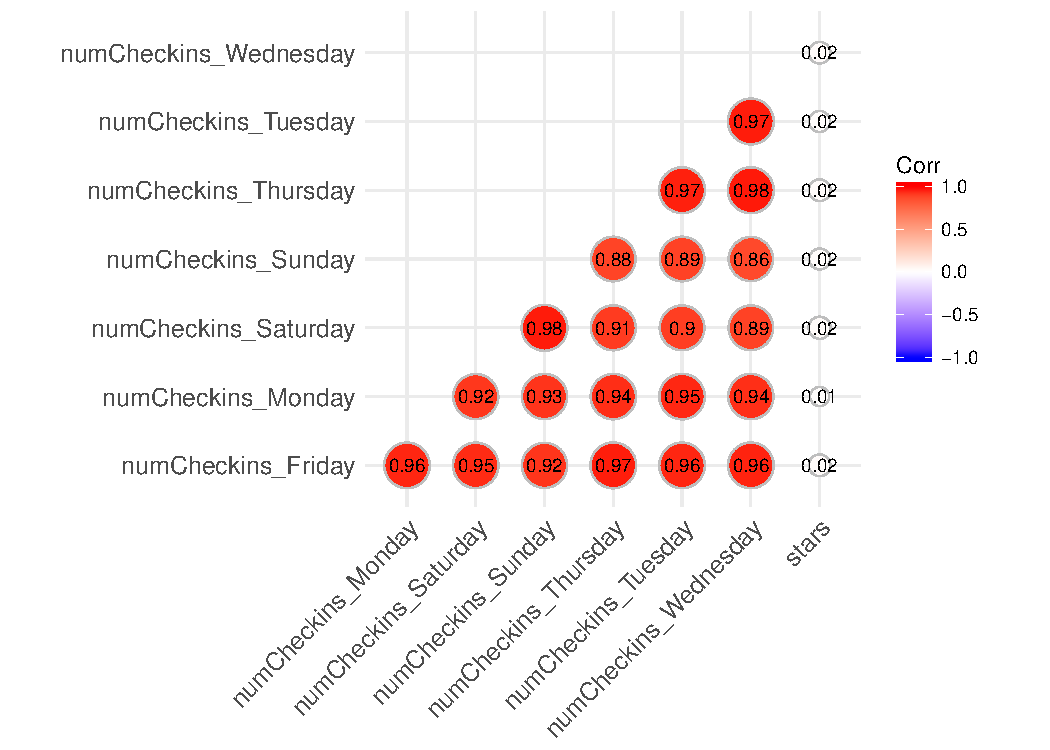
\includegraphics[width=\maxwidth]{figure/unnamed-chunk-42-1} 

\end{knitrout}



\begin{DIY}{Warning}
\noindent In order to use ggcorrplot(), the user will need to install the package as follows:\\
\noindent devtools::install\textunderscore github("kassambara/ggcorrplot")
\end{DIY}

\begin{DIY}{Homework}
  \begin{itemize}
  \item Generate the boxplot for all seven days and generate the plot as shown below
\begin{knitrout}
\definecolor{shadecolor}{rgb}{0.969, 0.969, 0.969}\color{fgcolor}
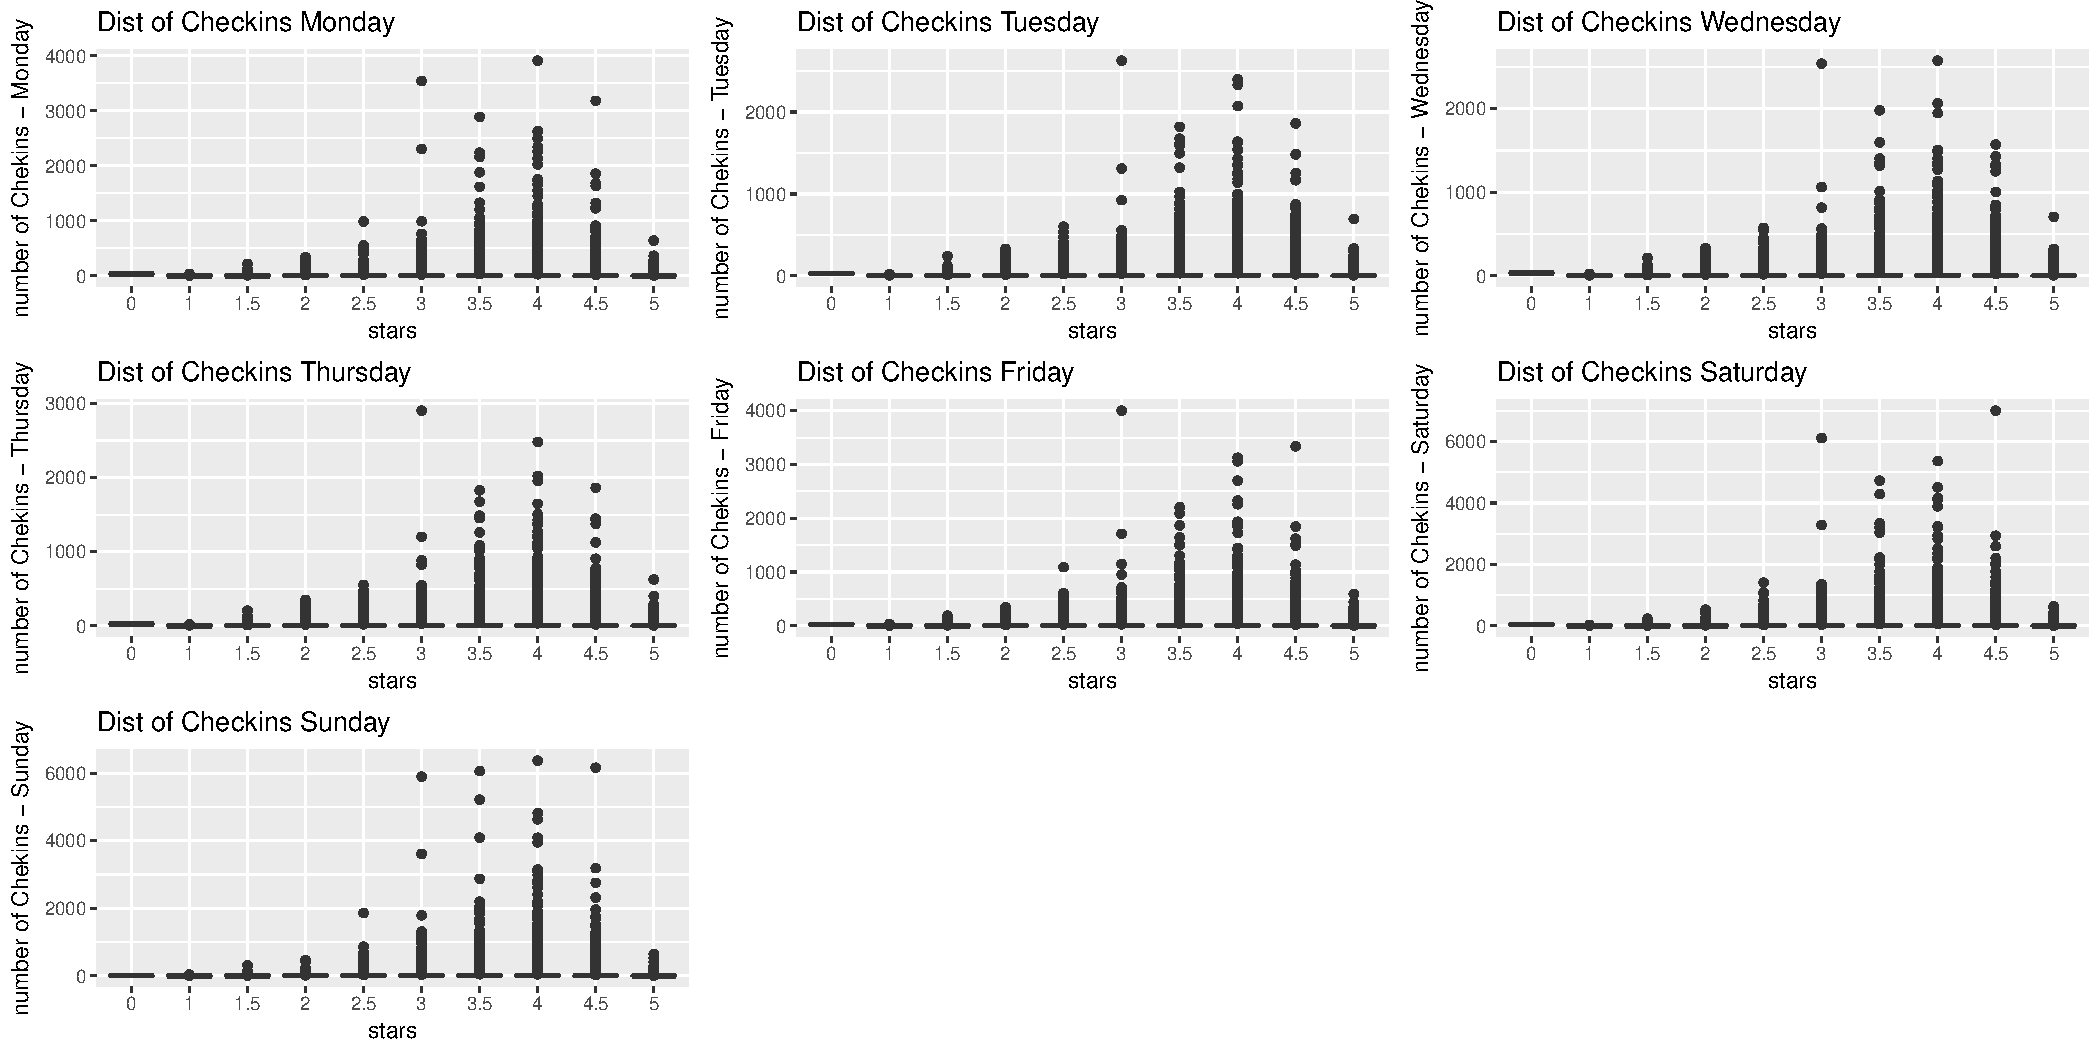
\includegraphics[width=\maxwidth]{figure/unnamed-chunk-44-1} 

\end{knitrout}
  \item Do the same for reviews i.e detect outliers in checkins while using reviews as a grouping variable. Moreover generate the correlation plot matrix and box plot matrix for the same
\end{itemize}
\end{DIY}

\newpage
\noindent \textbf{\underline{Question}}: How can we remove outliers from the data?
\begin{knitrout}
\definecolor{shadecolor}{rgb}{0.969, 0.969, 0.969}\color{fgcolor}\begin{kframe}
\begin{alltt}
\hlcom{## a function to returns the third quartile value grouped }
\hlcom{## by another variable}
\hlcom{## the function accepts the following arguments}
\hlcom{## input_ =  the vector whose summary statistics needs to }
\hlcom{##           be computed}
\hlcom{## groupingVec = the vector containing values on which }
\hlcom{##          we need to group the  values in input_ vector}
\hlcom{## returns: the third quartile of each group  }
\hlstd{getOutlierThresholds} \hlkwb{<-} \hlkwa{function}\hlstd{(}\hlkwc{input_}\hlstd{,}\hlkwc{groupingVec}\hlstd{)\{}
  \hlstd{result} \hlkwb{<-} \hlkwd{aggregate}\hlstd{(input_,}\hlkwc{by} \hlstd{=} \hlkwd{list}\hlstd{(groupingVec),summary)}
  \hlcom{## compute the summary statistics of input_ when grouped }
  \hlcom{## by the vales in groupingVec}
  \hlcom{## returns a list where the first element is the grouping}
  \hlcom{## values while the second element is the }
  \hlstd{summaryStats} \hlkwb{<-} \hlstd{result[,}\hlnum{2}\hlstd{]}
  \hlstd{groupingVals} \hlkwb{<-} \hlstd{result[,}\hlnum{1}\hlstd{]}
  \hlkwd{return}\hlstd{(summaryStats[,}\hlnum{5}\hlstd{])}
\hlstd{\}}


\hlstd{thresholdsPerRating} \hlkwb{<-} \hlkwd{apply}\hlstd{(trainingSet[,}\hlnum{2}\hlopt{:}\hlnum{8}\hlstd{],}
                             \hlnum{2}\hlstd{,}
                             \hlstd{getOutlierThresholds,}
                             \hlkwc{groupingVec}\hlstd{=trainingSet}\hlopt{$}\hlstd{stars)}
\hlcom{##apply the function getOutlierThresholds() on each of the }
\hlcom{## numChekins__ columns of trainingSet and group by }
\hlcom{## the attribute "stars"}

\hlstd{thresholdsPerRating} \hlkwb{<-} \hlkwd{data.frame}\hlstd{(}\hlstr{"stars"} \hlstd{=}
                                    \hlkwd{sort}\hlstd{(}\hlkwd{unique}\hlstd{(trainingSet}\hlopt{$}\hlstd{stars)),}
                                   \hlstd{thresholdsPerRating)}
\hlcom{## add the attribute "stars" to the data and create a data frame}

\hlcom{## a function to filter data based on }
\hlcom{## input conditions}
\hlcom{## the function accepts the following arguments}
\hlcom{## input_ =  A vector of size 2 that contains  }
\hlcom{##           (a) attribute filter  }
\hlcom{##           (b) value threshold}
\hlcom{## dataVec1 = the vector on which the }
\hlcom{##        attribute filter has to be applied}
\hlcom{## dataVec2 = the vector on which the }
\hlcom{##        threshold filter has to be applied}
\hlcom{## returns: vector of logicals, where the values }
\hlcom{## in positions that satisfy the conditions }
\hlcom{## are set to FALSE}
\hlstd{removeOutliers} \hlkwb{<-} \hlkwa{function}\hlstd{(}\hlkwc{input_}\hlstd{,}\hlkwc{dataVec1}\hlstd{,}\hlkwc{dataVec2}\hlstd{)\{}
  \hlstd{rating} \hlkwb{<-} \hlstd{input_[}\hlnum{1}\hlstd{]}
  \hlstd{threshold} \hlkwb{<-} \hlstd{input_[}\hlnum{2}\hlstd{]}
  \hlstd{idxVec} \hlkwb{<-}  \hlkwd{rep}\hlstd{(}\hlnum{TRUE}\hlstd{,}\hlkwd{length}\hlstd{(dataVec1))}
  \hlstd{idxVec[dataVec2} \hlopt{==} \hlstd{rating} \hlopt{&} \hlstd{dataVec1} \hlopt{>} \hlstd{threshold]} \hlkwb{<-} \hlnum{FALSE}
  \hlkwd{return}\hlstd{(idxVec)}
\hlstd{\}}

\hlstd{result} \hlkwb{<-} \hlkwd{apply}\hlstd{(thresholdsPerRating[,}\hlkwd{c}\hlstd{(}\hlstr{"stars"}\hlstd{,}\hlstr{"numCheckins_Friday"}\hlstd{)],}
                \hlnum{1}\hlstd{,removeOutliers,}
                \hlkwc{dataVec1} \hlstd{= trainingSet}\hlopt{$}\hlstd{numCheckins_Friday,}
                \hlkwc{dataVec2} \hlstd{= trainingSet}\hlopt{$}\hlstd{stars)}
\hlcom{## apply the function removeOutliers() to each row of the }
\hlcom{## first two columns of the thresholdsPerRating data frame }
\hlcom{## The vectors on which the conditions have to be applied}
\hlcom{## are passed on dataVec1 and dataVec2.}
\hlcom{## the result is a logical matrix of dimensions}
\hlcom{##  length(stars) X dim(thresholdsPerRating)[1] }
\hlcom{## the columns in result corresponds to }
\hlcom{## the value of star}

\hlstd{outliers_numCheckins_Friday} \hlkwb{<-} \hlkwd{apply}\hlstd{(result,}\hlnum{1}\hlstd{,prod)}
\hlcom{## For a given row of result, if either one of }
\hlcom{## the condition is satisfied  }
\hlcom{## (i.e one of the columns = FALSE), }
\hlcom{## the value should be filtered out. Therefore}
\hlcom{## we take a columnwise product}

\hlstd{cleanedTrainingSet} \hlkwb{<-} \hlstd{trainingSet[}\hlkwd{as.logical}\hlstd{(outliers_numCheckins_Friday),]}
\hlcom{## Filter all records from the trainingSet that ae not }
\hlcom{## outliers}

\hlstd{graph1} \hlkwb{<-} \hlkwd{boxplotMatrix}\hlstd{(base_graph,} \hlcom{##the base graph}
                        \hlkwd{aes}\hlstd{(}\hlkwc{x} \hlstd{=}
                              \hlkwd{as.factor}\hlstd{(cleanedTrainingSet}\hlopt{$}\hlstd{stars),}
                            \hlkwc{y} \hlstd{= cleanedTrainingSet}\hlopt{$}\hlstd{numCheckins_Monday}
                        \hlstd{),} \hlcom{## aesthetics mapping}
                        \hlstr{"stars"}\hlstd{,}\hlstr{"number of Chekins - Monday"}\hlstd{,}
                        \hlstr{"Dist of Checkins Monday"}\hlstd{)}
\hlkwd{ggcorrplot}\hlstd{(}\hlkwd{cor}\hlstd{(cleanedTrainingSet[,subsetCols]),} \hlcom{## }
            \hlkwc{method} \hlstd{=} \hlstr{"circle"}\hlstd{,}
           \hlkwc{type} \hlstd{=}\hlstr{"lower"}\hlstd{,}\hlkwc{lab} \hlstd{=} \hlnum{TRUE}\hlstd{,}
           \hlkwc{lab_size} \hlstd{=} \hlnum{3}\hlstd{)}
\end{alltt}
\end{kframe}
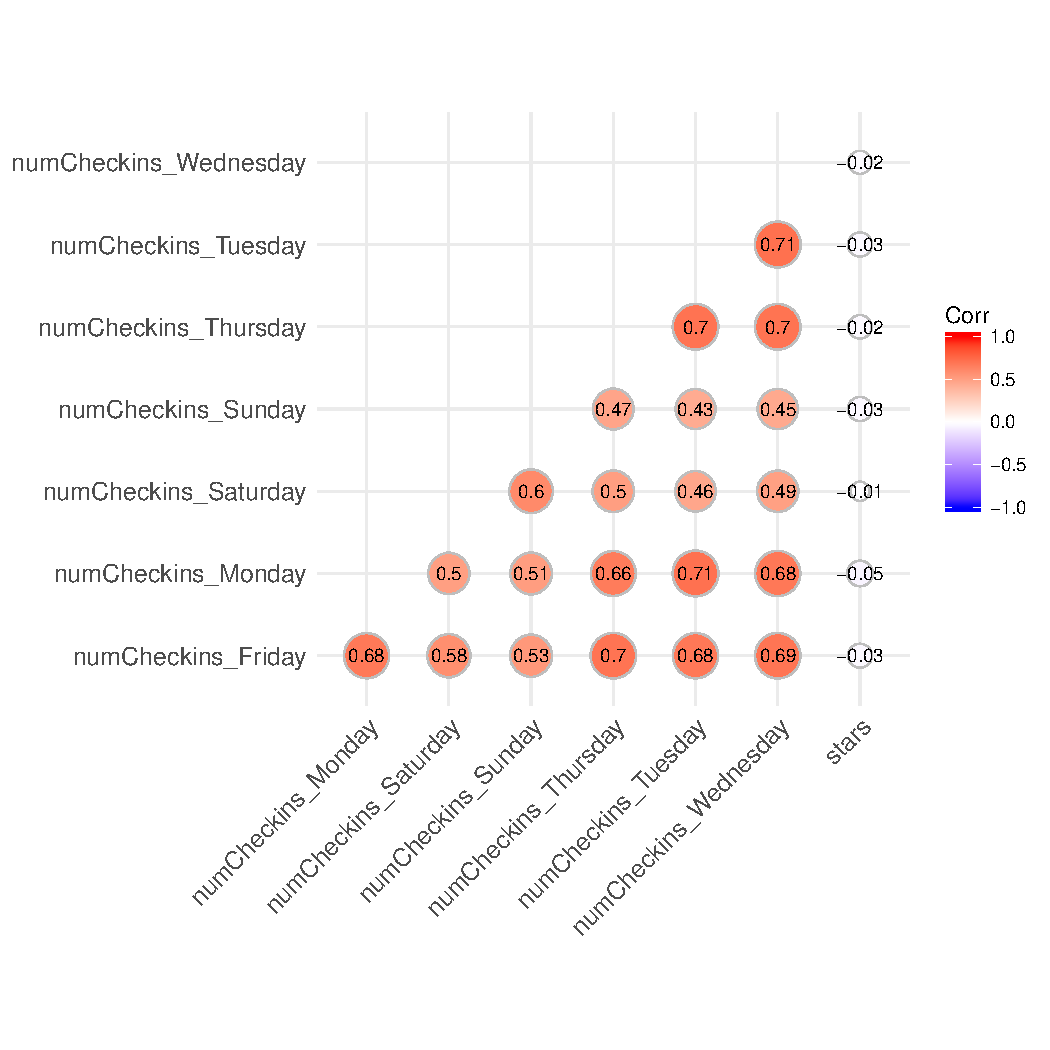
\includegraphics[width=\maxwidth]{figure/unnamed-chunk-45-1} 

\end{knitrout}


\begin{DIY}{Homework}
\noindent Generate the boxplot for all seven days (without the outliers) as shown below
\begin{knitrout}
\definecolor{shadecolor}{rgb}{0.969, 0.969, 0.969}\color{fgcolor}
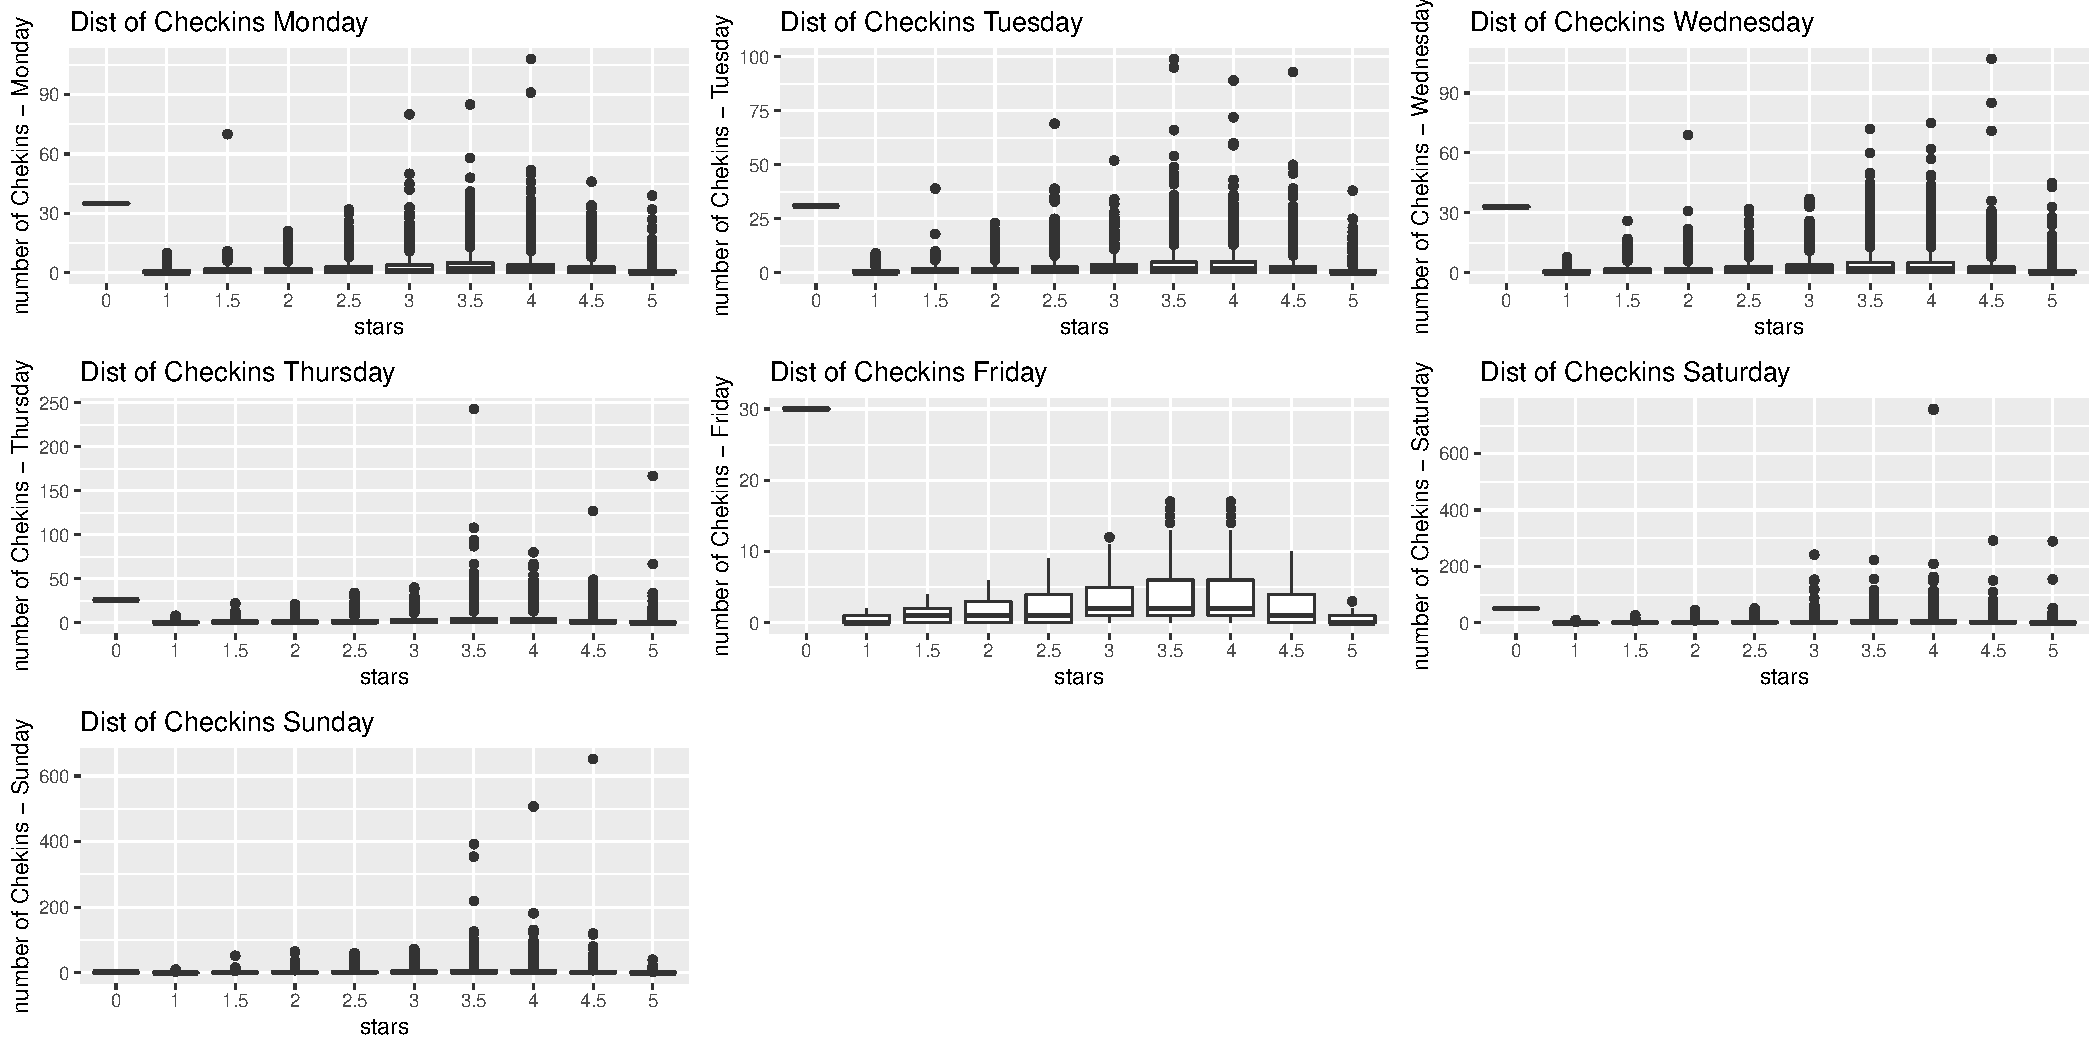
\includegraphics[width=\maxwidth]{figure/unnamed-chunk-47-1} 

\end{knitrout}
\end{DIY}

\begin{DIY}{Homework}
  \begin{itemize}
  \item Generate the correlation matrix for rest of the features wrt the outcome variable. What do you observe? 
  \item Are there features that have low correlation among themselves but high correlation with the outcome variable? Make a list of these features.
   \item Using the function that your wrote in \ref{sec:functions}, add the following features to the data i.e
   \begin{enumerate}
      \item number of checkins on weekdays
      \item number of checkins on weekends
      \item number of checkins during morning
      \item number of checkins during evening
      \item top5 states
   \end{enumerate}
   \item  Analyze the new features, namely
   \begin{enumerate}
        \item Check for presence of outliers wrt to the outcome variable.Remove the outliers. Generate relevant plots to demonstrate the same. 
        \item Check the correlation among these feature and wrt to the outcome variable. Explain your observation.
    \end{enumerate}
\end{itemize}
\end{DIY}

\newpage
%==================================================
\subsection{Setting up a Linear Regression Model}
%==================================================
\noindent \textbf{\underline{Question}}: How can we do linear regression?
\begin{knitrout}
\definecolor{shadecolor}{rgb}{0.969, 0.969, 0.969}\color{fgcolor}\begin{kframe}
\begin{alltt}
\hlstd{modelFull} \hlkwb{<-} \hlkwd{lm}\hlstd{(stars} \hlopt{~} \hlstd{. ,} \hlkwc{data} \hlstd{= trainingSet[,}\hlnum{2}\hlopt{:}\hlnum{59}\hlstd{])}
\hlcom{## fit a linear regression model on the full data where the }
\hlcom{## outcome variable is the number of stars}
\hlstd{predictedStars} \hlkwb{<-} \hlkwd{predict.lm}\hlstd{(modelFull,testSet[,}\hlnum{2}\hlopt{:}\hlnum{58}\hlstd{])}
\hlcom{## use the fitted model to predict the star of a business  }
\hlstd{squaredError} \hlkwb{<-} \hlstd{(testSet}\hlopt{$}\hlstd{stars} \hlopt{-} \hlstd{predictedStars)}\hlopt{^}\hlnum{2}
\hlstd{MeanSquaredError} \hlkwb{<-} \hlkwd{mean}\hlstd{(squaredError)}
\hlcom{## Calculate the mean squared error between the acutal rating}
\hlcom{## and predicted rating}
\hlstd{MeanSquaredError}
\end{alltt}
\begin{verbatim}
## [1] 0.733
\end{verbatim}
\begin{alltt}
\hlstd{modelOutlierRemoved} \hlkwb{<-} \hlkwd{lm}\hlstd{(stars} \hlopt{~} \hlstd{. ,}
                          \hlkwc{data} \hlstd{= cleanedTrainingSet[,}\hlnum{2}\hlopt{:}\hlnum{59}\hlstd{])}
\hlcom{## fit a linear regression model on the outlier removed data}
\hlcom{## outcome variable is the number of stars}
\hlstd{predictedStars} \hlkwb{<-} \hlkwd{predict.lm}\hlstd{(modelOutlierRemoved,testSet[,}\hlnum{2}\hlopt{:}\hlnum{58}\hlstd{])}
\hlcom{## use the fitted model to predict the star of a business}
\hlstd{squaredError} \hlkwb{<-} \hlstd{(testSet}\hlopt{$}\hlstd{stars} \hlopt{-} \hlstd{predictedStars)}\hlopt{^}\hlnum{2}
\hlstd{MeanSquaredError} \hlkwb{<-} \hlkwd{mean}\hlstd{(squaredError)}
\hlcom{## Calculate the mean squared error between the acutal rating}
\hlcom{## and predicted rating}
\hlstd{MeanSquaredError}
\end{alltt}
\begin{verbatim}
## [1] 1.11
\end{verbatim}
\end{kframe}
\end{knitrout}

\begin{DIY}{Think}
\noindent  Why do we see a higher mean squared error even after removing the outliers?
\end{DIY}

\begin{DIY}{Homework}
\begin{itemize}
  \item Setup a linear regression model by only considering the features that you have found useful in the previous section. Do you observe a change in the RMSE?
  \item Do the same by considering the outcome variable as reviews
  \item In \ref{sec:centering}, we converted ratings to a binary vector indicating whether it is above or below
  the average. Setup a regression model using this as the outcome variable. Make sure you do feature analysis wrt this outcome variable. 
\end{itemize}
\end{DIY}


\newpage
\includepdf[pages={1,2}]{./References/data-visualization-ggplot.pdf}

\end{document}
